% !Mode:: "TeX:UTF-8"

%\def\usewhat{dvipdfmx} % 定义编译方式 pdflatex, dvipdfmx, or xelatex
\def\usewhat{xelatex} % 定义编译方式 pdflatex, dvipdfmx, or xelatex


\def \xuewei{Master} % 定义学位 Doctor or Master

\def\xueke{Engineering} % 定义学科 Engineering, Science, Management, Arts, Philosophy, Economics, Laws, Education, or History

\documentclass[cs4size,openany,twoside,UTF8]{ctexbook}

% !Mode:: "TeX:UTF-8" 

\makeatletter
\@tempcnta=128
\loop \catcode\@tempcnta=13 \ifnum\@tempcnta<255 \advance \@tempcnta \@ne
\repeat
\makeatother

\newif\ifxueweidoctor %判断论文类型
\newif\ifxueweimaster
\def\temp{Doctor}
\ifx\temp\xuewei
  \xueweidoctortrue  \xueweimasterfalse
\fi
\def\temp{Master}
\ifx\temp\xuewei
  \xueweidoctorfalse  \xueweimastertrue
\fi

\ifxueweidoctor
  \newcommand{\cxuewei}{博士}
  \newcommand{\exuewei}{Doctor}
  \newcommand{\exueweier}{Doctoral}
  \newcommand{\xueweishort}{博}
\fi

\ifxueweimaster
  \newcommand{\cxuewei}{硕士}
  \newcommand{\exuewei}{Master}
  \newcommand{\exueweier}{Master}
  \newcommand{\xueweishort}{硕}
\fi    % 硕博类型
% !Mode:: "TeX:UTF-8"
\usepackage{ctex}
\usepackage{graphicx,cite,epsfig,amssymb,amsmath,color,epstopdf,epsfig}
\usepackage[a4paper,text={150true mm,224true mm},top=35.5true mm,left=30true mm,head=5true mm,headsep=2.5true mm,foot=8.5true mm]{geometry}
\usepackage{titlesec}               % 控制标题的宏包
\usepackage{titletoc}                   % 控制目录的宏包
\usepackage{fancyhdr}                   % fancyhdr宏包 页眉和页脚的相关定义
\usepackage{color}          % 支持彩色
\usepackage{amsmath}        % AMSLaTeX宏包 用来排出更加漂亮的公式
%\usepackage{amssymb}
\usepackage[below]{placeins}%允许上一个section的浮动图形出现在下一个section的开始部分,还提供\FloatBarrier命令,使所有未处理的浮动图形立即被处理
\usepackage{flafter}       % 使得所有浮动体不能被放置在其浮动环境之前,以免浮动体在引述它的文本之前出现.
\usepackage{multirow}       %使用Multirow宏包,使得表格可以合并多个row格
\usepackage{booktabs}       % 表格,横的粗线;\specialrule{1pt}{0pt}{0pt}
\usepackage{longtable}      %支持跨页的表格。
\usepackage{tabularx}
\usepackage{subfigure}%支持子图 %centerlast 设置最后一行是否居中
\usepackage[subfigure]{ccaption} %支持双语标题
\usepackage[sort&compress,numbers]{natbib}% 支持引用缩写的宏包
\usepackage{enumitem}       %使用enumitem宏包,改变列表项的格式
\usepackage{calc}           %长度可以用+ - * / 进行计算
\usepackage{txfonts}
\usepackage{bm}              % 处理数学公式中的黑斜体的宏包
\usepackage[amsmath,thmmarks,hyperref]{ntheorem}% 定理类环境宏包,其中 amsmath 选项用来兼容 AMS LaTeX 的宏包
\usepackage{float}
% 生成有书签的pdf及其开关, 该宏包应放在所有宏包的最后, 宏包之间有冲突
\def\atemp{dvipdfmx}\ifx\atemp\usewhat
\usepackage[dvipdfmx,unicode,           %dvi-->pdf 生成书签
            bookmarksnumbered=true,
            bookmarksopen=true,
            colorlinks=false,
            pdfborder={0 0 1},
            citecolor=blue,
            linkcolor=red,
            anchorcolor=green,
            urlcolor=blue,
            breaklinks=true
            ]{hyperref}
\fi

\def\atemp{pdflatex}\ifx\atemp\usewhat
\usepackage{cmap}                       %pdflatex编译时,可以生成可复制、粘贴的中文PDF文档
\usepackage[pdftex,unicode,
            %CJKbookmarks=true,
            bookmarksnumbered=true,
            bookmarksopen=true,
            colorlinks=false,
            pdfborder={0 0 1},
            citecolor=blue,
            linkcolor=red,
            anchorcolor=green,
            urlcolor=blue,
            breaklinks=true
            ]{hyperref}
\fi

\def\atempxetex{xelatex}\ifx\atempxetex\usewhat %\def\atempxetex{xelatex} main.tex中已定义;
\usepackage[xetex,
            bookmarksnumbered=true,
            bookmarksopen=true,
            colorlinks=false,
            pdfborder={0 0 1},
            citecolor=blue,
            linkcolor=red,
            anchorcolor=green,
            urlcolor=blue,
            breaklinks=true,
            naturalnames  %与algorithm2e宏包协调
            ]{hyperref}
\fi

\usepackage[ruled,algochapter]{algorithm2e}  % 算法的宏包,注意宏包兼容性,先后顺序为float、hyperref、algorithm(2e),否则无法生成算法列表
 % 引用的宏包

\graphicspath{{figures/}} %定义所有的eps文件在 figures 子目录下
\usepackage{fontspec}
\setmainfont{Times New Roman}
\begin{document}

% !Mode:: "TeX:UTF-8"

\newcommand{\song}{\CJKfamily{zhsong}}    % 宋体   (Windows自带simsun.ttf)
\newcommand{\fs}{\CJKfamily{fs}}        % 仿宋体 (Windows自带simfs.ttf)
\newcommand{\kai}{\CJKfamily{zhkai}}      % 楷体   (Windows自带simkai.ttf)
\newcommand{\hei}{\CJKfamily{zhhei}}      % 黑体   (Windows自带simhei.ttf)
\newcommand{\li}{\CJKfamily{li}}        % 隶书   (Windows自带simli.ttf)

\newcommand{\yihao}{\fontsize{26pt}{26pt}\selectfont}       % 一号, 1.倍行距
\newcommand{\xiaoyi}{\fontsize{24pt}{24pt}\selectfont}      % 小一, 1.倍行距
\newcommand{\erhao}{\fontsize{22pt}{1.25\baselineskip}\selectfont}       % 二号, 1.倍行距
\newcommand{\xiaoer}{\fontsize{18pt}{18pt}\selectfont}      % 小二, 单倍行距
\newcommand{\sanhao}{\fontsize{16pt}{16pt}\selectfont}      % 三号, 1.倍行距
\newcommand{\xiaosan}{\fontsize{15pt}{15pt}\selectfont}     % 小三, 1.倍行距
\newcommand{\sihao}{\fontsize{14pt}{14pt}\selectfont}       % 四号, 1.0倍行距
\newcommand{\xiaosi}{\fontsize{12pt}{12pt}\selectfont}      % 小四, 1.倍行距
\newcommand{\wuhao}{\fontsize{10.5pt}{10.5pt}\selectfont}   % 五号, 单倍行距
\newcommand{\xiaowu}{\fontsize{9pt}{9pt}\selectfont}        % 小五, 单倍行距


%避免宏包 hyperref 和 arydshln 不兼容带来的目录链接失效的问题。
\def\temp{\relax}
\let\temp\addcontentsline
\gdef\addcontentsline{\phantomsection\temp}

\makeatletter
\gdef\hitempty{}

%重新定义BiChapter命令,可实现标题手动换行,但不影响目录
\def\BiChapter{\relax\@ifnextchar [{\@BiChapter}{\@@BiChapter}}
\def\@BiChapter[#1]#2#3{\chapter[#1]{#2}
    \addcontentsline{toe}{chapter}{\bfseries \xiaosi Chapter \thechapter\hspace{0.5em} #3}}
\def\@@BiChapter#1#2{\chapter{#1}
    \addcontentsline{toe}{chapter}{\bfseries \xiaosi Chapter \thechapter\hspace{0.5em}{\boldmath #2}}}

\newcommand{\BiSection}[2]
{   \section{#1}
    \addcontentsline{toe}{section}{\protect\numberline{\csname thesection\endcsname}#2}
}

\newcommand{\BiSubsection}[2]
{    \subsection{#1}
    \addcontentsline{toe}{subsection}{\protect\numberline{\csname thesubsection\endcsname}#2}
}

\newcommand{\BiSubsubsection}[2]
{    \subsubsection{#1}
    \addcontentsline{toe}{subsubsection}{\protect\numberline{\csname thesubsubsection\endcsname}#2}
}

\newcommand{\BiAppendixChapter}[2] % 该附录命令适用于发表文章,简历等
{\phantomsection
\markboth{#1}{#1}
\addcontentsline{toc}{chapter}{\xiaosi #1}
\addcontentsline{toe}{chapter}{\bfseries \xiaosi #2}  \chapter*{#1}
}

\newcommand{\BiAppChapter}[2]    % 该附录命令适用于有章节的完整附录
{\phantomsection
 \chapter{#1}
 \addcontentsline{toe}{chapter}{\bfseries \xiaosi Appendix \thechapter~~#2}
}

\renewcommand{\thefigure}{\arabic{chapter}-\arabic{figure}}%使图编号为 7-1 的格式 %\protect{~}
\renewcommand{\thesubfigure}{\alph{subfigure})}%使子图编号为 a)的格式
\renewcommand{\p@subfigure}{\thefigure~} %使子图引用为 7-1 a) 的格式,母图编号和子图编号之间用~加一个空格
\renewcommand{\thetable}{\arabic{chapter}-\arabic{table}}%使表编号为 7-1 的格式
\renewcommand{\theequation}{\arabic{chapter}-\arabic{equation}}%使公式编号为 7-1 的格式

\def\BibTeX{\textsc{Bib}\kern-.08em\TeX}

\newcommand{\algoenname}{Algo.} %算法英文标题
\newfloatlist[chapter]{algoen}{aen}{\listalgoenname}{\algoenname}
\newfixedcaption{\algoencaption}{algoen}
\renewcommand{\thealgoen}{\thechapter-\arabic{algocf}}
\renewcommand{\@cftmakeaentitle}{\chapter*{\listalgoenname\@mkboth{\bfseries\listalgoenname}{\bfseries\listalgoenname}}}

\renewcommand{\algorithmcfname}{算法}
\setlength\AlCapSkip{1.2ex}
\SetAlgoSkip{1pt}
\renewcommand{\algocf@captiontext}[2]{\wuhao#1\algocf@typo ~ \AlCapFnt{}#2} % text of caption
\expandafter\ifx\csname algocf@within\endcsname\relax% if \algocf@within doesn't exist
\renewcommand\thealgocf{\@arabic\c@algocf} % and the way it is printed
\else%                                    else
\renewcommand\thealgocf{\csname the\algocf@within\endcsname-\@arabic\c@algocf}
\fi
\renewcommand{\algocf@makecaption}[2]{%中英文双标题一定多于一行,因此去掉单行时的判断,并将\parbox中标题设置为居中
  \addtolength{\hsize}{\algomargin}%
  \sbox\@tempboxa{\algocf@captiontext{#1}{#2}}%
    \hskip .5\algomargin%
    \parbox[t]{\hsize}{\centering\algocf@captiontext{#1}{#2}}%
  \addtolength{\hsize}{-\algomargin}%
}
\newcommand{\AlgoBiCaption}[2]{%直接取出自定义的中英文标题条目加入到真正的\caption 中
   \caption[#1]{\protect\setlength{\baselineskip}{1.5em}#1 \protect \\ Algo. \thealgocf~~ #2} % \algoencaption{#2}
   \addcontentsline{aen}{algoen}{\protect\numberline{\thealgoen}{#2}}
   }

\makeatother

%定义 学科 学位
\def \xuekeEngineering {Engineering}
\def \xuekeScience {Science}
\def \xuekeManagement {Management}
\def \xuekeArts {Arts}
\def \xuekePhilosophy {Philosophy}
\def \xuekeEconomics {Economics}
\def \xuekeLaws {Laws}
\def \xuekeEducation {Education}
\def \xuekeHistory {History}


\ifx \xueke \xuekeEngineering
\newcommand{\cxueke}{工程}
\newcommand{\exueke}{Engineering}
\fi

\ifx \xueke \xuekeScience
\newcommand{\cxueke}{理学}
\newcommand{\exueke}{Science}
\fi

\ifx \xueke \xuekeManagement
\newcommand{\cxueke}{管理学}
\newcommand{\exueke}{Management}
\fi

\ifx \xueke \xuekeArts
\newcommand{\cxueke}{文学}
\newcommand{\exueke}{Arts}
\fi

\ifx \xueke \xuekePhilosophy
\newcommand{\cxueke}{哲学}
\newcommand{\exueke}{Philosophy}
\fi

\ifx \xueke \xuekeEconomics
\newcommand{\cxueke}{经济学}
\newcommand{\exueke}{Economics}
\fi

\ifx \xueke \xuekeLaws
\newcommand{\cxueke}{法学}
\newcommand{\exueke}{Laws}
\fi

\ifx \xueke \xuekeEducation
\newcommand{\cxueke}{教育学}
\newcommand{\exueke}{Education}
\fi

\ifx \xueke \xuekeHistory
\newcommand{\cxueke}{历史学}
\newcommand{\exueke}{History}
\fi
 % 文本格式定义
% !Mode:: "TeX:UTF-8"

\theoremstyle{plain}
\theorembodyfont{\song\rmfamily}
\theoremheaderfont{\hei\rmfamily}
\newtheorem{definition}{\hei 定义}[chapter]
\newtheorem{example}{\hei 例}[chapter]
\newtheorem{algo}{\hei 算法}[chapter]
\newtheorem{theorem}{\hei 定理}[chapter]
\newtheorem{axiom}{\hei 公理}[chapter]
\newtheorem{proposition}{\hei 命题}[chapter]
\newtheorem{lemma}{\hei 引理}[chapter]
\newtheorem{corollary}{\hei 推论}[chapter]
\newtheorem{remark}{\hei 注解}[chapter]
\newenvironment{proof}{\noindent{\hei 证明:}}{\hfill $ \square $ \vskip 4mm}
\theoremsymbol{$\square$}
\setlength{\theorempreskipamount}{0pt}
\setlength{\theorempostskipamount}{-2pt}

\allowdisplaybreaks[4]

%\CJKcaption{gb_452}
%\CJKtilde
\setlength{\parindent}{2em}

\arraycolsep=1.6pt

\renewcommand\contentsname{\hei 目~~~~录}

\renewcommand\chaptername{\CJKprechaptername~\thechapter~\CJKchaptername}

\setcounter{secnumdepth}{4} \setcounter{tocdepth}{2}


\titleformat{\chapter}{\center\xiaoer\hei}{第\,\thechapter\,章}{1em}{}
\titlespacing{\chapter}{0pt}{-5.5mm}{8mm}
\titleformat{\section}{\xiaosan\hei}{\thesection}{0.5em}{}
\titlespacing{\section}{0pt}{4.5mm}{4.5mm}
\titleformat{\subsection}{\sihao\hei}{\thesubsection}{0.5em}{}
\titlespacing{\subsection}{0pt}{4mm}{4mm}
\titleformat{\subsubsection}{\xiaosi\hei}{\thesubsubsection}{0.5em}{}
\titlespacing{\subsubsection}{0pt}{0pt}{0pt}

\titlecontents{chapter}[3.8em]{\hspace{-3.8em}\hei}{\thecontentslabel\ }{}{\titlerule*[4pt]{.}\contentspage}
\dottedcontents{section}[40pt]{}{22pt}{0.3pc}
\dottedcontents{subsection}[62pt]{}{32pt}{0.3pc}


% 按工大标准, 缩小目录中各级标题之间的缩进,使它们相隔一个字符距离,也就是12pt
\makeatletter
\renewcommand*\l@chapter{\@dottedtocline{0}{0em}{4em}}%控制英文目录: 细点\@dottedtocline  粗点\@dottedtoclinebold
\renewcommand*\l@section{\@dottedtocline{1}{1.5em}{1.8em}}
\renewcommand*\l@subsection{\@dottedtocline{2}{2.5em}{2.5em}}


% 定义页眉和页脚
\newcommand{\makeheadrule}{
\rule[7pt]{\textwidth}{0.75pt} \\[-23pt]
\rule{\textwidth}{2.25pt}}
\renewcommand{\headrule}{
    {\if@fancyplain\let\headrulewidth\plainheadrulewidth\fi
     \makeheadrule}}
\pagestyle{fancyplain}

%去掉章节标题中的数字
%%不要注销这一行,否则页眉会变成:“第1章1  绪论”样式
%\renewcommand{\chaptermark}[1]{\markboth{\chaptertitlename~\ #1}{}}
\fancyhf{}

%在book文件类别下,\leftmark自动存录各章之章名,\rightmark记录节标题
%% 页眉字号 工大要求 小五
%根据单双面打印设置不同的页眉;

\ifxueweidoctor
  \fancyhead[CO]{\song \xiaowu\leftmark}
  \fancyhead[CE]{\song \xiaowu 哈尔滨工业大学\cxueke\cxuewei 学位论文 }%
  \fancyfoot[C,C]{\xiaowu -~\thepage~-}
\else
  \fancyhead[CO]{\song \xiaowu 哈尔滨工业大学\cxueke\cxuewei 学位论文}
  \fancyhead[CE]{\song \xiaowu 哈尔滨工业大学\cxueke\cxuewei 学位论文}%
  \fancyfoot[C,C]{\xiaowu -~\thepage~-}
\fi

\renewcommand\frontmatter{\cleardoublepage
  \@mainmatterfalse
  \pagenumbering{Roman}}

% 调整罗列环境的布局
\setitemize{leftmargin=3em,itemsep=0em,partopsep=0em,parsep=0em,topsep=-0em}
\setenumerate{leftmargin=3em,itemsep=0em,partopsep=0em,parsep=0em,topsep=0em}

\newcommand{\citeup}[1]{\textsuperscript{\cite{#1}}}

% 定制浮动图形和表格标题样式
\captionnamefont{\wuhao}
\captiontitlefont{\wuhao}
\captiondelim{~~}
\captionstyle{\centering}
\renewcommand{\subcapsize}{\wuhao}
\setlength{\abovecaptionskip}{0pt}
\setlength{\belowcaptionskip}{0pt}

% 自定义项目列表标签及格式 \begin{publist} 列表项 \end{publist}
\newcounter{pubctr} %自定义新计数器
\newenvironment{publist}{%%%%%定义新环境
\begin{list}{[\arabic{pubctr}]} %%标签格式
    {
     \usecounter{pubctr}
     \setlength{\leftmargin}{2.5em}     % 左边界 \leftmargin =\itemindent + \labelwidth + \labelsep
     \setlength{\itemindent}{0em}     % 标号缩进量
     \setlength{\labelsep}{1em}       % 标号和列表项之间的距离,默认0.5em
     \setlength{\rightmargin}{0em}    % 右边界
     \setlength{\topsep}{0ex}         % 列表到上下文的垂直距离
     \setlength{\parsep}{0ex}         % 段落间距
     \setlength{\itemsep}{0ex}        % 标签间距
     \setlength{\listparindent}{0pt} % 段落缩进量
    }}
{\end{list}}%%%%%

% 默认字体
\renewcommand\normalsize{
  \@setfontsize\normalsize{12pt}{12pt}
  \setlength\abovedisplayskip{4pt}
  \setlength\abovedisplayshortskip{4pt}
  \setlength\belowdisplayskip{\abovedisplayskip}
  \setlength\belowdisplayshortskip{\abovedisplayshortskip}
  \let\@listi\@listI}

% 设置行距和段落间垂直距离
\def\defaultfont{\renewcommand{\baselinestretch}{1.62}\normalsize\selectfont}
\renewcommand{\CJKglue}{\hskip 0.56pt plus 0.08\baselineskip}
%加大字间距,使每行34个字,若要使得每行33个字,则将0.56pt替换为0.96pt。
\predisplaypenalty=0  %公式之前可以换页,公式出现在页面顶部

% 封面、摘要、版权、致谢格式定义
\def\ctitle#1{\def\@ctitle{#1}}\def\@ctitle{}
\def\cdegree#1{\def\@cdegree{#1}}\def\@cdegree{}
\def\caffil#1{\def\@caffil{#1}}\def\@caffil{}
\def\csubject#1{\def\@csubject{#1}}\def\@csubject{}
\def\cauthor#1{\def\@cauthor{#1}}\def\@cauthor{}
\def\csupervisor#1{\def\@csupervisor{#1}}\def\@csupervisor{}
\def\cassosupervisor#1{\def\@cassosupervisor{{\hei 副 \hfill 导 \hfill 师} & #1\\}}\def\@cassosupervisor{}
\def\ccosupervisor#1{\def\@ccosupervisor{{\hei 联 \hfill 合\hfill 导 \hfill 师} & #1\\}}\def\@ccosupervisor{}
\def\cdate#1{\def\@cdate{#1}}\def\@cdate{}
\long\def\cabstract#1{\long\def\@cabstract{#1}}\long\def\@cabstract{}
\def\ckeywords#1{\def\@ckeywords{#1}}\def\@ckeywords{}

\def\etitle#1{\def\@etitle{#1}}\def\@etitle{}
\def\edegree#1{\def\@edegree{#1}}\def\@edegree{}
\def\eaffil#1{\def\@eaffil{#1}}\def\@eaffil{}
\def\esubject#1{\def\@esubject{#1}}\def\@esubject{}
\def\eauthor#1{\def\@eauthor{#1}}\def\@eauthor{}
\def\esupervisor#1{\def\@esupervisor{#1}}\def\@esupervisor{}
\def\eassosupervisor#1{\def\@eassosupervisor{\textbf{Associate Supervisor:} & #1\\}}\def\@eassosupervisor{}
\def\ecosupervisor#1{\def\@ecosupervisor{\textbf{Co Supervisor:} & #1\\}}\def\@ecosupervisor{}
\def\edate#1{\def\@edate{#1}}\def\@edate{}
\long\def\eabstract#1{\long\def\@eabstract{#1}}\long\def\@eabstract{}
\long\def\NotationList#1{\long\def\@NotationList{#1}}\long\def\@NotationList{}
\def\ekeywords#1{\def\@ekeywords{#1}}\def\@ekeywords{}
\def\natclassifiedindex#1{\def\@natclassifiedindex{#1}}\def\@natclassifiedindex{}
\def\internatclassifiedindex#1{\def\@internatclassifiedindex{#1}}\def\@internatclassifiedindex{}
\def\statesecrets#1{\def\@statesecrets{#1}}\def\@statesecrets{}

% 定义封面
\def\makecover{
    \begin{titlepage}
    % 封面一
   \vspace*{0.8cm}
   \begin{center}
    %\centerline{\xiaoyi\song\textbf{\cxuewei 学位论文}}
    \begin{center}{\xiaoyi\song\textbf{\cxuewei 学位论文}}\end{center}

    \vspace{1cm}

    \parbox[t][2.8cm][t]{\textwidth}{
    \begin{center}\erhao\hei\@ctitle\end{center} }

    \parbox[t][5.1cm][t]{\textwidth}{ %英文标题太长时可以采用\xiaoer
    \begin{center}\erhao\bfseries{\@etitle}\end{center} }
    %\begin{center}\erhao\@etitle\end{center} }

    \parbox[t][7.4cm][t]{\textwidth}{
    \begin{center}\xiaoer\song\textbf{\@cauthor}\end{center}}

    \parbox[t][1.4cm][t]{\textwidth}{
    \begin{center}\kaishu\xiaoer\textbf{哈尔滨工业大学}\end{center} }

    {\song\xiaoer\textbf{\@cdate}}

    \end{center}

    % 封二 空白页
    \ifxueweidoctor
      \newpage
      ~~~\vspace{1em}
      \thispagestyle{empty}
    \fi

    %内封
    \newpage
    \thispagestyle{empty}

\begin{center}

			{\song \xiaosi
			\begin{tabular}{@{}r@{:}l@{}}
			国内图书分类号 & \@natclassifiedindex\\
 			国际图书分类号 & \@internatclassifiedindex
			\end{tabular}}\hfill
			{\song \xiaosi
			\begin{tabular}{@{}r@{:}l@{}}
			学校代码 & 10213\\
 			密级 &  公开
			\end{tabular}}
    \parbox[t][3.2cm][t]{\textwidth}{\begin{center} \end{center} }

    \parbox[t][2.4cm][t]{\textwidth}{\xiaoer
    \begin{center} {\song \bfseries \@cdegree 学位论文 }\end{center} }

    \parbox[t][5cm][t]{\textwidth}{\erhao
    \begin{center} {\hei  \@ctitle}\end{center} }
	\parbox[t][9.8cm][b]{\textwidth}
     {\sihao
    \begin{center} \renewcommand{\arraystretch}{1.62} \song
    \begin{tabular}{l@{:}l}
    {\hei \xueweishort \hfill 士\hfill 研\hfill 究\hfill 生}           & \@cauthor\\
    {\hei 导\hfill 师}                       & \@csupervisor\\
	\@cassosupervisor
	\@ccosupervisor
    {\hei 申\hfill 请\hfill 学\hfill 位} & \@cdegree\\
    {\hei 学\hfill 科}           & \@csubject\\
    {\hei 所\hfill 在\hfill 单\hfill 位} & \@caffil\\
    {\hei 答\hfill 辩\hfill 日\hfill 期} & \@cdate\\
    {\hei 授予学位单位}                     & 哈尔滨工业大学
    \end{tabular} \renewcommand{\arraystretch}{1}
    \end{center} }
\end{center}

%%%%%%增加一空白页
  \ifxueweidoctor
    \newpage
    ~~~\vspace{1em}
    \thispagestyle{empty}
  \fi

    % 英文封面
    \newpage
    \thispagestyle{empty}

    {
    \xiaosi\noindent Classif\/ied Index: \@natclassifiedindex \\
                  U.D.C:  \@internatclassifiedindex }
    \begin{center}
    \parbox[t][1.6cm][t]{\textwidth}{\begin{center} \end{center} }
    \parbox[t][3.5cm][t]{\textwidth}{\xiaoer
    \begin{center} {  Dissertation for the {\exueweier} Degree in Engineering}\end{center} } %与中文保持一致,删除in {\exueke}

    \parbox[t][7cm][t]{\textwidth}{\erhao
    \begin{center} { \bfseries \@etitle}\end{center} }

%★★★★若信息内容不太长,不会引起信息内容分行时,使用tabular环境,否则使用下面的tabularx环境。
    {\sihao\renewcommand{\arraystretch}{1.3}
    \begin{tabularx}{0.9\textwidth}{@{}l@{~}X@{}}
    \textbf{Candidate:}                     &  \@eauthor\\
    \textbf{Supervisor:}                    &  \@esupervisor\\
	  \@eassosupervisor
	  \@ecosupervisor
    \textbf{Academic Degree Applied for:}   &  \@edegree\\
    \textbf{Specialty:}                     &  \@esubject\\
    \textbf{Affiliation:}                   &  \@eaffil\\
    \textbf{Date of Defence:}               &  \@edate\\
    \textbf{Degree-Conferring-Institution:} &  Harbin Institute of Technology
    \end{tabularx}\renewcommand{\arraystretch}{1}}

    %{\sihao\renewcommand{\arraystretch}{1.3}
    %\begin{tabularx}{\textwidth}{@{}l@{~}X@{}}
    %\textbf{Candidate:}                     &  \@eauthor\\
    %\textbf{Supervisor:}                    &  \@esupervisor\\
		%\@eassosupervisor
	  %\@ecosupervisor
    %\textbf{Academic Degree Applied for:}   &  \@edegree\\
    %\textbf{Specialty:}                     &  \@esubject\\
    %\textbf{Affiliation:}                   &  \@eaffil\\
    %\textbf{Date of Defence:}               &  \@edate\\
    %\textbf{Degree-Conferring-Institution:} &  Harbin Institute of Technology
    %\end{tabularx}\renewcommand{\arraystretch}{1}}

    \end{center}
    \end{titlepage}

%%%%%%增加一空白页
  \ifxueweidoctor
    \newpage
    ~~~\vspace{1em}
    \thispagestyle{empty}
  \fi
%%%%%%%%%%%%%%%%%%%   Abstract and keywords  %%%%%%%%%%%%%%%%%%%%%%%
\clearpage

\BiAppendixChapter{摘\quad 要}{Abstract (In Chinese)}

\setcounter{page}{1}
\song\defaultfont
\@cabstract
\vspace{\baselineskip}

\hangafter=1\hangindent=52.3pt\noindent
{\hei 关键词:} \@ckeywords

%%%%%%%%%%%%%%%%%%%   English Abstract  %%%%%%%%%%%%%%%%%%%%%%%%%%%%%%
\clearpage

%\phantomsection
%\markboth{Abstract}{Abstract}
\addcontentsline{toc}{chapter}{\xiaosi ABSTRACT}
\addcontentsline{toe}{chapter}{\bfseries \xiaosi Abstract (In English)}  \chapter*{\textbf{Abstract}}
\@eabstract
\vspace{\baselineskip}

\hangafter=1\hangindent=60pt\noindent
{\textbf{Keywords:}}  \@ekeywords
}

%%%%%%%%%%%%%%%%%%%%%%%%%%%%%%%%%%%%%%%%%%%%%%%%%%%%%%%%%%%%%%%
% 英文目录格式
\def\@dotsep{0.75}           % 定义英文目录的点间距
\setlength\leftmargini {0pt}
\setlength\leftmarginii {0pt}
\setlength\leftmarginiii {0pt}
\setlength\leftmarginiv {0pt}
\setlength\leftmarginv {0pt}
\setlength\leftmarginvi {0pt}

\def\engcontentsname{\bfseries Contents}
\newcommand\tableofengcontents{
   \pdfbookmark[0]{Contents}{econtent}
     \@restonecolfalse
   \chapter*{\engcontentsname  %chapter*上移一行,避免在toc中出现。
       \@mkboth{%
          \engcontentsname}{\engcontentsname}}
   \@starttoc{toe}%
   \if@restonecol\twocolumn\fi
   }

\urlstyle{same}  %论文中引用的网址的字体默认与正文中字体不一致,这里修正为一致的。

\renewcommand\endtable{\vspace{-4mm}\end@float}

\makeatother


\frontmatter
% !Mode:: "TeX:UTF-8"

\newcommand{\chinesethesistitle}{密集热点区域无线网络性能分析与优化} %授权书用,无需断行
\newcommand{\englishthesistitle}{\uppercase{performance analysis and optimization in dense hot point wireless networks}} %\uppercase作用:将英文标题字母全部大写;
\newcommand{\chinesethesistime}{2018~年~6~月}  %封面底部的日期中文形式
\newcommand{\englishthesistime}{June, 2018}    %封面底部的日期英文形式

\ctitle{密集热点区域无线网络性能分析与优化}  %封面用论文标题,自己可手动断行
\cdegree{\cxueke\cxuewei}
\csubject{电子与通信工程}                 %(~按二级学科填写~)
\caffil{电子与信息工程学院} %(在校生填所在系名称,同等学力人员填工作单位)
\cauthor{麻津铭}
\csupervisor{陈晓华教授} %导师名字
%\cassosupervisor{副导名}%若没有,请屏蔽掉此句。
%\ccosupervisor{联导名}%若没有,请屏蔽掉此句。


\cdate{\chinesethesistime}

\etitle{\englishthesistitle}
\edegree{\exuewei \ of \exueke}
\esubject{Electronics and Communication Engineering}  %英文二级学科名
\eaffil{School of Electronics and \qquad \quad Information Engineering}
\eauthor{Ma Jin-Ming}                   %作者姓名 (英文)
\esupervisor{Prof. Hsiao-Hwa Chen}       % 导师姓名 (英文)
%\eassosupervisor{Prof. Assosuper}%若没有,请屏蔽掉此句。
%\ecosupervisor{Prof. Cosuper}%若没有,请屏蔽掉此句。
\edate{\englishthesistime}

\natclassifiedindex{TN929.53}  %国内图书分类号
\internatclassifiedindex{621.3}  %国际图书分类号
\statesecrets{公开} %秘密

\iffalse
\BiAppendixChapter{摘~~~~要}{}  %使用winedt编辑时文档结构图(toc)中为了显示摘要,故增加此句;
\fi
\cabstract{
第五代移动通信技术(~the 5~th Generation Communication Technology,5G~)将于2020年前后开始商用,
相比于第四代移动通信技术(~the 4th Generation Communication Technology,4G~),
5G~网络的容量需求将有~1000~倍的增长。
超密集组网(~Ultra Dense Networks, ~UDNs~)通过在区域内放置更多的微基站(~Small Base Station,SBS~)换取网络性能的提升,
是一种能够提供巨大容量增益的十分可靠的技术。
但是,超密集组网使~SBS~之间的距离更近,随之带来的~SBS~之间干扰问题越发明显。
在超密集组网场景中,由于~SBS~之间的距离较近,因此~SBS~和用户构成的通信链路的信道状态信息(~Channel State Information,CSI~)
易于汇总到控制端,再由控制端控制~SBS~进行数据的发送,达到~SBS~之间协作的目的。
由于协作的~SBS~的天线之间的距离远远大于天线的相关距离(~Coherence Distance~),
因此协作的~SBS~可以构成一个分布式的多输入多输出(~Multiple-Input Multiple-Output,MIMO~)系统,
协作的~SBS~所服务的用户可以通过波束成型(Beamforming,BF)的方法将用户的接收信号向量在空域上相互正交,
达到干扰消除的目的。

首先,本文对基于格的基站部署方法进行了研究,包括环形的基站部署方法和方格点的基站部署方法。
对上述两种基站部署方法的拓扑结构进行了介绍,并对性能进行了分析。
对于环形的基站部署方法,讨论了环的半径~$R$~和基站的个数~$N$~对整个网络的性能的影响。
对于方格点的基站部署方法,讨论了~SBS~之间的横向间距~$l_1$~和纵向间距~$l_2$~对网络的性能的影响。

接着,本文对基于泊松点过程(~Poisson Point Process,PPP~)的基站部署的性能进行了研究,
并假设用户的分布为混合二维高斯分布以反映网络中的用户的不均匀性和聚集性。
提出了一种简单可行的办法计算该场景下的覆盖率和单位面积频谱效率等性能指标,
并讨论了影响网络性能的相关参量。

本文最后对网络中用户的接收信干比(~Signal Inference Ratio,SIR~)性能做进一步的优化。
优化的过程分为两步,
第一步出于对网络的同步性和复杂度要求的考虑本文提出了基于深度优先搜索和以用户为中心的基站分簇算法,
第二步对簇内采用基于~SBS~间协作的分布式迫零预编码(~Zero-Forcing Beamforming,ZFBF~)技术优化网络中用户的接收~SIR,
应用仿真分析的方法讨论了优化后的网络的性能。
}
\ckeywords{超密集组网;随机几何;微基站分簇;联合传输;波束形成}

\eabstract{

The 5th-generation mobile communication technology(5G) will begin commercial application around 2020.
Compared to the 4th-generation mobile communication technology(4G),
the capacity requirement of the 5G network will increase by 1,000 times.
The ultra-dense networks(UDNS) improves the network performance by placing more base stations in the area.
It is a very reliable technology that can provide huge capacity gains.
However, the UDNs makes the distance between SBSs closer,
and the interference between ~SBSs~ gets more obvious.
In UDNs, since the distance between SBSs is relatively close,
 it is easier to get the channel state information (CSI) of the communication link formed by SBS
 and the user and submit to the controler.
The controler instructs SBSs to send data, achieving the cooperation between SBSs.
Since the distance between the antennas of the cooperative SBSs is much larger than the coherence distance of the antennas,
the cooperative SBSs can form a distributed multiple-input multiple-output (MIMO) system.
The users of the cooperative SBS can use the beamforming(BF) method to orthogonalize the user's received signal vectors in the space domain,
achieving the purpose of interference cancellation.

Firstly,the grid-based base station deployment methods are introduced, including the ring-shaped base station deployment method and the grid point base station deployment method.
The topology structure of the above two base station deployment methods is introduced and the performance is analyzed.
For the ring-shaped base station deployment method, the effect of the ring radius $R$ and the number of base stations $N$ on the performance of the entire network is discussed.
For the grid points base station deployment method,
the influence of the horizontal spacing between SBSs $l_1$ and the vertical spacing $l_2$ on the performance of the network is discussed.

Next, the performance of base station deployments based on the Poisson Point Process(PPP) is discussed.
It is assumed that the user's distribution is a mixed two-dimensional Gaussian distribution to reflect the user's heterogeneity and aggregation in the network.
A tractable method is proposed to calculate the coverage area rate and spectral efficiency  under this scenario.
And related parameters that affect network performance are discussed.

Finally, the user's receive signal-to-interference ratio (SIR) performance in the network is optimizated.
The optimization process is divided into two steps.
At the first step, considering the requirements of synchronization and complexity of the network,
clustering based on th depth-first search and user-centric clustering algorithm are proposed.
At the second step is  the Zero-Forcing Beamforming (ZFBF) technique based on SBS cooperation are used to optimize the user's receive~SIR in the network,
besides, simulation analysis is used to discuss the performance of the optimized network.
}

\ekeywords{UDNs, Stochastic Geometry, Clustering, CoMP, Beamforming}


\makecover
\clearpage

\BiAppendixChapter{附~~~~表}{}
{
%\begin{longtable}[c]{@{}ccc@{}}
%
%\end{longtable}
%\toprule[1.5pt]
%变量名       &  & 物理意义\tabularnewline
%\midrule[1pt]
%\endhead
%$A$         &  & 区域的面积\tabularnewline
%$\alpha$    &  & 路径损耗系数\tabularnewline
%$\Phi$      &  & 微基站的分布\tabularnewline
%$\lambda_s$ &  & 微基站的密度\tabularnewline
%$P$         &  & 微基站的最大发射功率\tabularnewline
%$\Psi$      &  & 用户的分布\tabularnewline
%$\lambda_u$ &  & 用户的密度\tabularnewline
%$h$         &  & 瑞利信道衰落系数\tabularnewline
%$d$         &  & 用户和基站之间的距离\tabularnewline
%\bottomrule[1.5]
%\end{longtable}
\begin{table}[htbp]
\label{sinr_sim_para}
\vspace{0.5em}\centering\wuhao
\begin{tabular}{cccc}
\toprule[1.5pt]
变量名 & & & 物理意义 \\
\midrule[0.5pt]
$A$         & & & 区域的面积\tabularnewline
$\alpha$    & & & 路径损耗系数\tabularnewline
$\Phi$      & & & 微基站的分布\tabularnewline
$\lambda_s$ & & & 微基站的密度\tabularnewline
$P$         & & & 微基站的最大发射功率\tabularnewline
$\Psi$      & & & 用户的分布\tabularnewline
$\lambda_u$ & & & 用户的密度\tabularnewline
$h$         & & & 瑞利信道衰落系数\tabularnewline
$d$         & & & 用户和基站之间的距离\tabularnewline
$\gamma$    & & & 用户的接收信干噪比\tabularnewline
$\delta$    & & & 用户的信干比需求门限\tabularnewline
$\tau$      & & & 基于深度优先搜索的基站分簇算法的距离门限\tabularnewline
$k$         & & & 基于~k~-~均值的基站分簇算法的均值个数\tabularnewline
$\mu$       & & & 以用户为中心的基站分簇算法的簇内最多基站数\tabularnewline
\bottomrule[1.5pt]
\end{tabular}
\end{table}
}
 % 封面

% 中英目录
\defaultfont
\clearpage{\pagestyle{empty}\cleardoublepage}
\pdfbookmark[0]{目~~~~录}{mulu}
\tableofcontents    % 中文目录
\clearpage{\pagestyle{empty}\cleardoublepage}

\ifxueweidoctor
\tableofengcontents % 英文目录 会出现错误
\fi


\clearpage{\pagestyle{empty}\cleardoublepage}     % 清除目录后面空页的页眉和页脚


\mainmatter\defaultfont\sloppy\raggedbottom

% !Mode:: "TeX:UTF-8"

\BiChapter{绪~~~~论}{Introduction}

\BiSection{课题背景及研究的目的和意义}{Background, aims and significance}
在未来的5G网络中,将会涌现出大量的智能移动终端,对网络的容量要求大大增加\citeup{QosUDN}。
相比于4G,5G网络的容量需求将有1000倍的增长,届时,终端无处不在,并且在大型的热点区域,如商场,露天展台等存在着大量的连接设备。
同时,不同的移动终端也会有不同的业务需求,这也就导致了业务需求的多样化。基站的密集部署迫在眉睫。
超密集组网应运而生。
超密集组网将用于满足区域面积内超高的容量需求,为移动终端提供无缝的网络切换,让用户在无论何时,无论何地都能拥有超高速的上网和通话体验。
超密集组网在区域面积内放置了更多的基站,这是能够提供巨大容量增益一种十分可靠的技术\citeup{4LRA}。
通过在宏基站的热点区域放置小的基站,也可以实现在小区内的任何地点都可以流畅通信的愿景。
超密集组网,在分层异构网络的基础上,部署高密度低功耗的小型网络来实现系统容量的大幅提升。

微小区网络和异构网络提供了更高的频谱自由度,有效的提高了系统的单位面积谱效率,从而提升了系统的性能。
微小区和异构网络也是实现超密集组网,应对未来高单位面积频谱利用率挑战的一种重要可行的手段\citeup{condesign}。
但微小区和异构网络的部署收到当地地形地貌的影响:有的地方地貌平坦,遮挡较少,适宜部署基站,有些地方地形崎岖,遮挡明显,不适宜部署基站。
微小区和异构网络的部署也受到当地人流的影响,有的地方客流量大,对容量的需求也就更加的高,因此该区域就需要密集的部署。
不仅如此,微小区和异构网络的部署也呈现自组织性。
种种原因导致了对微小区和异构网络的建模不能采用传统的基于格点的建模方式。\citeup{ATractable}。
同时由于用户在小区中的不同位置的概率不同,比如在某些热点区域,如展会中心区,景观区,用户分布较多,呈现从中间向四周蔓延的趋势,而在其他区域,用户不会有明显的集聚效应。
小区中的用户密度在不同时间也是不同的,如在高峰期,用户数远远大于基站数。
而在夜晚夜深人静的时候,用户数可能和基站数目相当甚至小于基站数。
因此要考虑联合统筹考虑基站和用户的统计分布特性,进而设计一个比格点分布更加可靠合理的模型。
去估计密集热点区域无线网络的性能。得到准确的网络性能边界。

密集的组网在带来好处的同时,也带来了新的挑战,密集的网络使得基站之间的距离更近,随之带来的小基站之间干扰问题越发明显。
不仅如此,网络复杂程度的增高也导致了小区中的频谱资源,功率资源的调度与协调变得越发复杂。
密集的组网也导致了很高的能耗\citeup{OFDMRA},小基站能提供的功率也不会像宏基站提供的功率那么强,有一定的约束,如何将有限的功率很好的利用,服务的用户更多,提供的容量更大,基站的耗能却更小,也是现在亟需解决的热点问题。
因此需要有新的干扰管理技术,新的资源分配和功率控制算法,充分协调现有的或者将要部署的小基站之间的关系,从而消除小基站之间的干扰,提升系统对用户的统计覆盖率,提升网络的单位面积频谱利用率,达到容量提升的目的。


本课题来源于国家自然科学基金,项目名称《超密集组网中区域频谱效率理论上界及干扰管理算法研究》(项目号:61671186)。

\BiSection{国内外研究现状及分析}{Background, aims and significance}

\BiSubsection{超密集组网的研究现状}{UDNs}
2009年,业界提出了第五代移动通信技术(5G)的概念。
在继承和发扬第四代移动通信技术(4G)的基础之上,5G系统的目标是提升几十被的频谱效率,百倍左右的能量效率,同时为了便于推广,5G系统也需要在成本上做出考虑。
5G中的关键技术——超密集组网技术,是目前业界各个知名厂家争相研究的热点\cite{zhanghong}。
网络异构化和密集化已经成为了当下移动无线组网的一个大趋势。

当前超密集组网的研究,由于超密集组网即是一种技术,优势一种场景,因此需要对该场景进行合理有效的建模并进行分析。
5G中的超密集组网,由于网络的拓扑结构复杂,呈现异构化,随机化,多层次,因此,不能按照传统的移动蜂窝网络,将基站建模成六边形格点的拓扑结构。
网络的建模要呈现随机性。文献\cite{ATractable}最早提出了能够体现随机化的无线多基站网络模型。
该篇文章考虑到由于网络的密集程度的提升,受到地理位置,区域对网络的需求等等随机化的影响,因此网络中基站的部署呈现随机性。
为了反应这种随机性,基于随机几何\citeup{Stogeo},提出了将基站的分布服从泊松点过程,而用户在区域内随机分布的网络拓扑模型。
并得到一种简单可行的方法,求解该场景下的终端概率、区域面积谱效率等等性能。
但该篇文章只考虑了单小区单层单天线多基站,用户数量远远大于基站数量的情况\citeup{4LRA}。
文献\cite{2LayerPC}提出了单小区双层多基站超密集无线网络模型,并分析了该场景下的能耗特性。
文献\cite{UDNMIMO}在前两篇文章的基础上,提出了单小区多层异构的网络,小区中的基站配备多根天线。
该文献还考虑了基站数量和用户数量的关系。并重点分析了基站和用户数量相当的情况下网络的性能。
并给出了在该场景下的基站睡眠和唤醒机制的算法。给出了能达到最大单位面积谱效率下,小区内部署基站的密度。
文献\cite{user-centric}提出了以用户为中心的超密集组网的网络模型。该模型假设小区中的基站服从泊松点过程,小区中的用户随机分布,
小区中的用户的数量与基站的数量相当,或者小于基站的数量。该模型假设网络采用了干扰协调算法,
并假设距离用户最近的基站为用户进行服务,并设定一个距离门限,将距用户距离不超过距离门限的基站作为干扰协调基站。
用于协调其他用户和基站所建立的链路对该用户的影响。

随着通信技术的发展,移动通信无线网络的架构不断的更新改进。
网络的架构是网络中最关键的一个部分。针对超密集组网网络场景,需要选择一种合理的架构,并在该架构的基础上进行改进,更好的与超密集组网场景和现有的技术进行适配。
在当前主流的网络架构中,软件定义网络(SDN)、云接入网络(CRAN)、雾接入网络(FRAN)等架构各自具有优势,适合与现有的超密集组网网络场景进行结合。

软件定义网络技术是未来网络设计和资源管理方法的一个很有潜力的参考方法,它可以将网络的控制层与数据层分开\citeup{cbsdn}。
它将软件层面设计从硬件系统上剥离开来,使得不同的服务、不同的应用都可以采用一套软件系统进行处理。
文献\cite{condesign}探索了软件定义网络架构应用在超密集组网网络场景下的的可能。
通过统一的控制中心,让网络能够正常可靠的运转。同时每个边缘的基站负责传输数据,保证系统的高速有效的运行。
在超密集组网网络场景下,采用软件定义无线网络的架构,引用了博弈论和经济学的手段,设计了一种新的协议,该协议可以达到纳什均衡,优化了超密集组网场景的性能,使得网络中可以承载的最大用户数提升,并均衡了负载,提升了系统的鲁棒性。
文献\cite{CRANUDN}探索了CRAN网络架构应用于超密集无线组网网络场景下的可能性。

CRAN即云接入网络,最早由美国IT业的巨头公司IBM提出\citeup{MMCRAN},该网络架构将小区的基带处理单元(BBU)整合在一起,构成BBU池放在控制中心,
在需要部署基站的位置放置低复杂度的远拉射频头(RRH),远拉射频头用来对分布在小区中的需求用户进行服务,是一种非常有效的网络密集话的手段。
CRAN应用于超密集组网的场景下有很多的优点。CRAN网络架构是干扰协调和频谱资源管理的一种有效的方法,同时,由于RRH结构简单,RRH可以以较低的硬件成本进行密集的布放。
由于中心化的架构,多用户干扰可以被诸如CoMP这样的多点协作技术有效的解决掉,这样将会有很有效的性能增益。
在传统的CRAN架构中(4G),C-RAN被部署用于连接宏基站和BBU池,由于BBU和RRH之间的传输路径长,这种传统的基站会造成很大的传输时延,而在密集热点区域采用C-RAN架构,延迟也会被大大的缩短。
BBU池化后资源统一调度,有助于解决网络需求随时间改变的潮汐效应,有利于提高能量效率。
同时,CRAN技术应用在超密集组网网络场景下还有很多的方面有待改进,由于超密集组网的密集部署,网络系统需要进一步的减小功耗。
主要的手段是增加RRH睡眠与活跃状态的切换功能,并设计出合理的选择算法。
同时CRAN由于模拟端和数据端的分离,使得网络的正常运转需要前向链路对数字原始信号进行回传。为了适应超密集组网网络场景的需求,也需要设计低花费前向链路。
同时CRAN架构应用于超密集组网网络场景还需要进一步降低当前算法的计算复杂度,降低训练开销,并研究在不完整的CSI下的传输策略。
FRAN为最新提出的思想,在CRAN网络架构下,提出了去中心化和分布式的思想,在云接入网络架构的基础上,引入边缘计算技术,改进网络架构。

\BiSubsection{小区资源管理和调度算法的研究现状}{MIMO}

OFDM小区间干扰严重,与CDMA的区别,都有那些减小的技术

小区中的资源管理和调度算法,是伴随移动无线通信网络诞生开始就面临的一个难点。
由于频谱资源,时间资源,空间资源都是有限的,为了利用有限的网络资源,我们不得不采用将空间划分成为许多个小区,每个小区中放置基站对小区中的用户进行服务。
在前几代蜂窝移动通信网络中,采用频率复用技术解决小区之间的干扰问题。

蜂窝移动通信网络初期,由于网络中服务的用户量较小,网络众多用户对容量的需求较低,设备较为落后。小区之间多采用较为简单的频率复用的调度方法。
相邻的小区之间采用不同的频谱资源,每个小区所分配的频谱资源相同。这样的好处是可以几乎彻底的解决小区之间的干扰。
但是同样的,由于每个小区所分配的频谱资源相同且固定不利于针对不同小区之间容量需求的不均匀的情况,网络的自适应调节能力较差。
由于相邻的小区采用不同的频谱资源,导致小区的可用频谱资源降低一倍以上,因此虽然提升了小区内用户的统计覆盖率,但是,
去使小区的单位面积谱效率有较大的损失。而超密集组网网络场景下,网络系统需要满足大连接,高速率的需求,区域面积频谱利用率显然是一个非常重要的指标。
在静态频率复用的基础之上,出现了更加复杂的基于频率复用的小区资源管理和调度算法。

在众多频率复用算法中,软频率复用是一种可靠的频率复用技术,该技术由华为提出\citeup{yangxuezhi},并应用与4G组网的场景下。软频率复用是传统的复用技术的改进。
软频率复用技术,通过设定发射功率门限,区分不同频率的使用。这样做,使得相邻的小区不一定要使用完全不同的频率资源,而是只需要相邻小区的边缘用户使用不同的频率。
而小区中心的用户距离相邻基站的距离较远,收到相邻基站的影响较小,因此虽然使用相同的频率资源,但实际上用户与服务基站构成的通信链路并不会受到相邻基站的干扰的强烈的影响。

软频率复用的方法虽然解决了之前频率复用系统频谱利用率较低的问题,但是用于小区中的频谱资源是固定的,并没有考虑小区与小区之间的网络容量需求不均匀的问题,因此网络的动态性较差。
由于硬件性能的提升,网络机构的逐渐发展。小区与小区之间可以共享一部分信息,并且中心控制器也可以控制多个小区,因此,可以采用单个中心控制器控制多个小区,将多个小区的资源混合在一起做一个统筹。
多个小区之间进行动态的频率复用。基于该思想,文献\cite{4LRA}提出了一种多小区动态频率资源分配的算法,该算法基于图论的思想,应用贪婪算法对图中的节点进行着色,完成频率资源的分配。
但是该频率资源分配算法采用贪婪算法,不能达到性能的最优,需要进一步的引入小区中基站的分布规律和分布特点,以及用户的分布规律和特点。
引入比贪婪算法更优秀的图论优化的算法达到性能的最优。

预编码技术也是进行干扰管理和消除的一个重要的技术。
预编码最早由Tomlinson提出,用于单输入单输出(SISO)系统当中。
预编码的主要思想是由于发射机多为基站,其提供的功率很高,这就允许了基站可以做的很复杂,许多算法可以在基站端实现的话,就可以减少很多手机终端的负担。
除此之外,由于基站端知道所有用户的信道状态信息,因此,基站可以利用所得到的信道状态信息进行干扰消除。
由于不同的用户和基站构成的信道链路不相同,因此由信道状态因数构成的信道矩阵可以构成一个向量空间,
根据预编码技术,用户所发送的信息可以等效为向量空间中的一个向量,可以利用向量与向量之间的相关性来刻画不同链路之间的干扰。
预编码就是利用信道状态信息,使得多个天线之间组成的链路尽量的正交。
文献\cite{DisPrecode}发明了一种分布时预编码的预编码算法,由于超密集组网的特性,网络中的基站较为密集,这也就使得不同的基站之间可以共享部分信道状态信息。
系统可以等效为一个多输入多输出(MIMO)系统。应用预编码技术,用户之间的干扰会有显著的降低。
文献\cite{LayerPrecode}和\cite{Layer2Precode}采用分层的方法,首先进行单小区的分析,之后进行多小区的预编码,虽然采用分层次的预编码技术不能够使得性能达到最优。
但是采用层次化的设计,可以在每一层都可以达到局部的最优或次优,却显著的降低了算法的复杂度。

不仅如此,基于超密集组网场景的特性,基站的部署较为密集,因此,经常会出现用户的数量与基站的数量相当,或者用户的数量与基站的数量相比更少。
因此在5G系统中,引入了以用户为中心的联合传输策略。其主要的思想是去距离用户近信道信息较好的基站为服务基站。而其他的接收功率大于预设门限的基站作为干扰协调的基站,协调其他用户与基站之间构成的链路对该用户的干扰。
文献\cite{Ucent}提出了以用户为重新的干扰管理算法,并且引入了联合传输技术,用户的总的接收功率有了显著的提升,干扰的功率有了显著的降低。
文献\cite{CoMPUDN}提出了基于多点联合传输(CoMP)的干扰管理算法,提出以用户为中心的干扰管理算法。通过仿真,文中证明以用户为中心的干扰管理算法有效的缓解了小区间的干扰。
文献\cite{UNOMAcent}采用以用户为中心的策略,针对超密集组网网络场景,结合最新的非正交多址(NOMA)调制技术。文章通过仿真证明了系统的单位面积频谱效率有了显著的提升。

虽然小区资源管理和调度算法已经被研究多年,但由于超密集组网网络场景的提出,网络的场景越来越复杂,再加上近几年许多新的网络架构的出现。
为了解决当下稀缺的频谱资源与不断增加的用户和用户需求之间的矛盾。必须要设计出一套新的干扰管理和资源分配算法,协调小区间的干扰,增加单位面积的频谱利用率,提高网络的能量效率。


\BiSubsection{国内外研究现状简析}{Analysis}
超密集组网是5G中的重要的技术,5G要覆盖主要的三个场景,即高速率场景,大连接场景,低时延场景。
而超密集组网网络是解决在大连接的情况下,满足网络中的用户能在很高的速率之下运行。
因此研究超密集组网网络场景下的技术,在5G中有着至关重要的作用。
在当下,调制技术,编码技术等5G中关键的技术都已经基本的确定了,5G研究的中心也逐渐转移至网络层。

网络层面上,随着第五代移动通信技术的发展与推广以及计算机领域和电子硬件领域的进步,网络架构层面上,也有了很多发展。
其中CRAN技术、FRAN技术、异构网络技术、软件定义网络(SDN)技术都有潜力为超密集组网的网络架构提供网络架构层面的参考。
但是现在还没有一个已经确定的针对超密集组网网络场景下的一个很好的优化方案。
在超密集组网的网络架构中,要避免网络消耗过大,前向链路容量需求过大,计算复杂度过高,延时过高的现有网络架构的不足。
还有能够支持大连接高速率的需求。

由于网络的干扰管理算法从移动蜂窝网络发明和推广开始就一直是组网的重点问题。
但目前并没有很好的针对超密集组网网络场景的特性,进行合理优化的比较有效的算法。



\BiSection{本文研究内容及组织结构}{Content and structure}
本文首先对超密集组网中用到的基本的技术进行阐述和探究。对超密集组网网络场景中有潜力的技术进行了总结,对关键参数进行了深入的讨论。
接着,根据超密集组网网络场景的特性。
针对网络中基站和用户的统计特性,对密集热点区域无线网络的网络场景进行了建模分析,得到了理论上的网络覆盖率和单位面积频谱利用效率的边界。
最后,针对超密集组网的网络场景,网络拓扑结构,网络统计特性,基于二分图模型,提出了一种低复杂度的资源分配和干扰管理算法。
仿真证明,该资源分配和干扰管理算法复杂度较之前算法更低,并且支持的用户数和系统的和容量好于传统同复杂度的算法。
章节安排如下:

第~1~章:介绍课题背景及研究的目的和意义,叙述国内外在超密集组网和干扰管理和资源分配算法两方面的研究现状以及存在的问题,给出本文的研究内容。

第~2~章:对超密集组网网络场景中可行的网络架构和合理的系统模型进行了介绍,对关键参数进行了深入的讨论。

第~3~章:针对网络中基站和用户的统计特性,对密集热点区域无线网络的网络场景进行了建模分析,得到了理论上的网络覆盖率和单位面积频谱利用效率的边界。

第~4~章:针对密集热点区域无线网络的网络特性,对网络进行优化,首先采用分簇算法对基站进行分簇,接着对将统一簇内的基站
通过~CRAN~网络架构进行联合,对簇内采用基于~ZFBF~的多用户联合传输技术。
仿真结果证明,该干扰管理策略有效地优化了网络的覆盖率和单位面积频谱效率的性能。

% !Mode:: "TeX:UTF-8"

\BiChapter{规则的微基站部署的性能分析}{architecture and system model}

本章介绍规则的微基站部署,
这也是网络部署的一种基本的方法。
该方法分为两个步骤,首先在服务区域~$\mathcal{D}$~中选定固定格点,
然后在选定的格点上部署微基站。
常见的规则的微基站部署有环形部署和方格部署,
在进行分析之前,首先对网络中的关键性能指标进行描述,
然后分别对上述不同的基站部署的拓扑结构进行介绍和性能分析。

\BiSection{超密集组网通信的性能指标}{matrices}
本小节介绍衡量超密集组网的通信性能的主要指标,其中包括信干噪比、遍历容量、覆盖率和单位面积谱效率。

\BiSubsection{信干噪比}{SINR}

可靠性和有效性一直是评定通信性能的一个重要指标。其中有效性可以通过网络的信道容量进行衡量。而网络的信道容量是一个直接与信干噪比有关的量。
信干噪比的表达式如~(\ref{SINR})~所示:
\begin{equation}\label{SINR}
  \mathrm{SINR}=\frac{P}{I+N}
\end{equation}
其中~$P$~为通信链路中接收机的接收功率,~$I$~为其他的通信链路对该通信链路所造成的干扰。$\mathrm{SINR}$~表示该通信链路的信干噪比。

超密集组网区域用户与基站之间距离比较近,因此干扰占有几乎全部的比重,反之噪声的影响几乎可以忽略不计,
也就是说,超密集组网场景是一个干扰受限的信道。其信干比近似等于信干燥比。信干比的表达式如~(\ref{SIR})~:
\begin{equation}\label{SIR}
  \mathrm{SIR}=P/I
\end{equation}
其中~$\mathrm{SIR}$~表示该通信链路的接收信干比。本篇文章假设小区中用户的接收信干噪比与信干比相等。
\BiSubsection{用户的遍历容量}{ASE}
给定一个用户的接收信干比,即可以求出一个用户的遍历容量,在平稳的瑞利信道下,用户的遍历容量如式~\ref{e_capacity_formular}~所示:
\begin{equation}\label{e_capacity_formular}
  C_{Rayleigh} = \int_{0}^{\infty} B \log_2(1+\mathrm{SINR}(h)) f(h) \mathrm{d} h
\end{equation}
其中~$C_{Rayleigh}$~为瑞利信道的遍历容量,~$f(h)$~为~$h$~的概率密度分布函数,$B$~为信道的带宽。信道的遍历容量表示一个用户在一段时间内,遍历所有可能性下的信道容量的统计平均值。
因为信道为瑞利信道,因此在固定位置上的用户,由于受到了信道系数的影响,其信干噪比在不同的时间点上也是不同的,又由于瑞利信道是平稳的信道,
因此可以采用遍历所有信道系数的可能性得到的统计均值代替时间上的遍历,用~$\mathrm{SINR}(h))$~表示。

遍历容量可以反应一个用户在一段时间内通信的有效性,是反应网络性能的重要指标。

\BiSubsection{区域覆盖率}{Coverage}
为保证用户的服务质量与速率要求,用户的接收信干比需要维持在一个固定的门限上,而到底有多少用户在该时刻上有很好的信干比,或者说在瞬时上能达到所要求的信干比的用户一共有多少呢?区域覆盖率是评定的有效的指标。
区域覆盖率的定义如~(\ref{pc})~所示:
\begin{equation}\label{pc}
  p_c(T) = \mathbf{P}[\mathrm{SINR}>T]
\end{equation}
其中~$T$~为给定的信干噪比的门限,~$\mathrm{SINR}$~为通信链路的信干噪比,$\mathbb{P}$~表示概率。根据定义,可对其物理意义做出以下的三种解释:

 (1)~服务用户的信干噪比为以上的概率。

 (2)~信干噪比为以上的用户占总用户的百分比。

 (3)~信干噪比为以上的区域占总区域的百分比。

覆盖率是评定无线网络性能的一个重要的概念,并且根据覆盖率,可以很容易的得到有能达到给定的速率要求在整个区域中的所有用户的占比。
同时该物理量也是单位区域上信干噪比的概率分布函数的补函数。
\BiSubsection{区域面积谱效率}{ASE}

香农定理给出了通信系统的理论容量上界\citeup{TheMathematicalTheoryOfCommunication},表达式如~(\ref{shannon})~所示:
\begin{equation}\label{shannon}
  C = B \log_2(1+\mathrm{SINR})
\end{equation}

式~(\ref{shannon})~中,~$C$~ 代表理论的容量的上界也即系统最大的传输速率, $B$ 代表信道的带宽, ~$\mathrm{SINR}$~ 代表接收端信号的信干噪比。
香农定理可以解释现代各种无线制式由于带宽不同,所支持的单载波最大吞吐量的不同。香农公式表达了在给定带宽下,噪声和干扰都服从高斯分布的情况下,系统所能达到的理论最大容量。

频谱效率的定义为单位带宽上所能承载的最大的吞吐量,如~(\ref{SE})~所示:
\begin{equation}\label{SE}
\eta_{SE}=C/B=\log_2(1+\mathrm{SINR})
\end{equation}
上式中~$C/B$~就是单位带宽的容量,单位为~$bps/\mathrm{Hz}$~体现信道链路的传输性能。式~(\ref{SE})~给出了理论上频谱效率的理论最大值。

在密集热点区域无线网络的场景中,单个链路的容量已经不再是衡量一个网络的好坏的唯一指标,在超密集组网场景中,还要考虑在一段时间内,网络中服务的用户的和容量。
同时,考虑到不同区域上的频谱效率相差可能非常悬殊。因此在密集热点的网络环境下,频谱效率将不能够完全反映整个区域的无线网络的性能,
取而代之的是单位面积谱效率这一物理量,其定义为在单位面积上的频谱效率,表达式如~(\ref{ASE})~所示:
\begin{equation}\label{ASE}
  \eta_{ASE}=C/(B\cdot S) = \lambda_s~\mathbb{E}[\log_2(1+\mathrm{SINR})]
\end{equation}
单位为~$bps/\mathrm{Hz}/\mathrm{m}^2$~。其中~$\lambda_s$~为服务区域内基站的密度。区域面积谱效率的物理意义为单位面积上所承载的平均的和容量。

\BiSection{环形的基站部署}{Defination of UDNs}

\BiSubsection{环形的基站部署的拓扑结构}{Defination of UDNs}
环形基站部署将基站部署在一个圆环上,其特别适合大型比赛场馆,大型演唱会等场景下的基站部署。
环形的基站部署方法的示意图如图~\ref{single_circle_bs_show}~所示,
在区域~$\mathcal{D}$~上,选定半径~$R$,在半径为~$R$~的圆上均匀的部署~$N$~个基站,
在图~\ref{single_circle_bs_show}~中,
$\mathcal{D}$~为一个~$100\mathrm{m}\times 100 \mathrm{m}$~的区域,
部署基站的半径大小~$R=30\mathrm{m}$,基站的个数~$N=12$~个。
\begin{figure}[htbp]
\centering
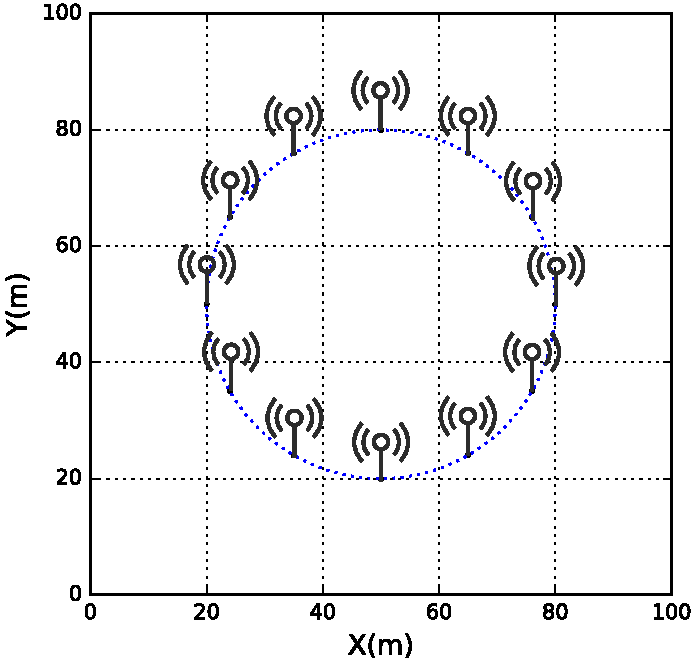
\includegraphics[width = 0.62\textwidth]{single_circle_bs_station.pdf}
\caption{环形基站部署的拓扑结构示意图}\vspace{-0.5em}
\label{single_circle_bs_show}
\end{figure}
若微基站同时同频的传送信息,
则由于在中心处的用户距所有基站的距离均比较近,
因此在未采用任何基站协作的前提下,若以就近原则选择服务的基站,
处在中心处的用户受到除服务基站以外的其他基站的干扰非常严重,
但由于处在距离环比较近的用户距离服务基站的距离较近,因此接收信号较强,
用户的接收信干噪比较好,处在圆环区域附近的用户的覆盖性能是较好的。
在环形基站的部署当中,基站的个数~$N$~和圆环的大小~$R$~以及服务区域的面积的大小均是
有关系的,由于网络模型复杂,不易对网络的各个性能求出闭合解,
但是可以用蒙特卡洛仿真的方法分析网络的性能,下面对在不同的参数条件下的基站环形部署的性能进行分析。

\BiSubsection{环形的基站部署的遍历容量}{Defination of UDNs}
对环形基站的遍历容量分布图进行蒙特卡洛仿真分析,
仿真的参数表如表~\ref{single_circle_sinr_sim_para}~所示,
\begin{table}[htbp]
\caption{遍历容量的热力分布图的仿真参数}
\label{single_circle_sinr_sim_para}
\vspace{0.5em}\centering\wuhao
\begin{tabular}{cccc}
\toprule[1.5pt]
参量 & & & 设置 \\
\midrule[0.5pt]
区域~$\mathcal{D}$~的大小  & & & ~$100\mathrm{m} \times 100 \mathrm{m}$~ \\
信道的类型 & & &  瑞利衰落信道\\
基站的个数~$N$~ & & &  12\\
圆环的半径~$R$~ & & &  ${30\mathrm{m}}$\\
信道衰落系数~$\alpha$~  & & & 2,~4\\
\bottomrule[1.5pt]
\end{tabular}
\end{table}
该仿真主要反应了瑞利信道下的区域内的各个位置的遍历容量的特性,
而遍历容量是一个与信干比相关的量,
因此仿真结果可以反应每个区域上的信干比的特性。
基站的个数、圆环的大小、区域的大小固定,通过遍历容量热力分布图可以得到信道衰落系数对网络的遍历容量的性能的影响,
采用蒙特卡洛仿真,得到的结果如图~\ref{single_circle_e_capacity_show}~所示,
\begin{figure}[htbp]
\centering
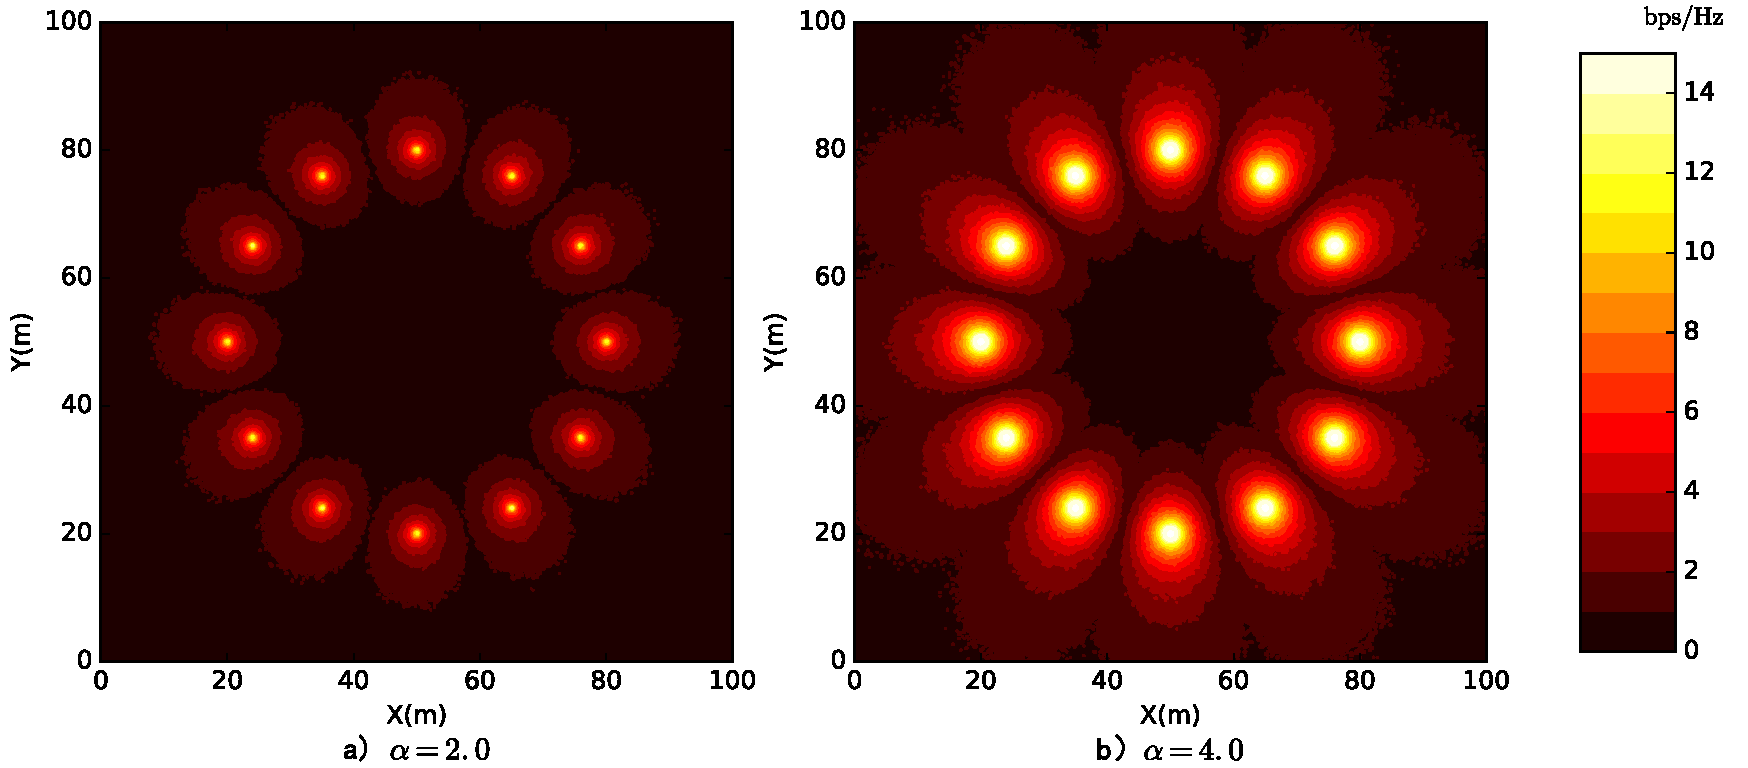
\includegraphics[width = 0.90\textwidth]{single_circle_e_capacity_show_30_12.pdf}
\caption{环形基站部署的遍历容量热力图}\vspace{-0.5em}
\label{single_circle_e_capacity_show}
\end{figure}
可以看到距离服务基站较近的用户的遍历容量较好,
当~$\alpha=4$~时,距离微基站大概~$3\mathrm{m}$~以内的用户的遍历容量均大于~$10\mathrm{bps/Hz}$。
整个区域的热力分布图呈现辐射状,信道衰减系数大的辐射的更远,处在中心处的用户的性能很差,
遍历容量小于~$1\mathrm{bps/Hz}$。

\BiSubsection{环形的基站部署的覆盖率的性能分析}{Defination of UDNs}
我们在上一小节讨论了路径损耗因子对性能的影响,
接下来对网络的覆盖率性能采用蒙特卡洛仿真分析,对网络的覆盖率性能进行分析,
主要分析环形基站部署的两个重要指标,即圆环的半径~$R$和基站的个数~$N$对基站的覆盖率的影响。
同时,由于用户在区域内的分布不一定是均匀的,因此需要对不同用户的分布情况进行分析,
考虑用户的分布~$\Psi$~分别为随机分布和以微基站的位置坐标为均值的二维高斯分布的情况。
仿真的参数表如表~\ref{single_circle_pc_sim_para}~所示,
\begin{table}[htbp]
\caption{覆盖率的仿真参数}
\label{single_circle_pc_sim_para}
\vspace{0.5em}\centering\wuhao
\begin{tabular}{cccc}
\toprule[1.5pt]
参量 & & & 设置 \\
\midrule[0.5pt]
区域~$\mathcal{D}$~的大小  & & & ~$100\mathrm{m} \times 100 \mathrm{m}$ \\
信道的类型 & & &  瑞利衰落信道\\
基站的个数~$N$~ & & &  8, 16\\
圆环的半径~$R$~ & & &  ${30\mathrm{m}},{50\mathrm{m}}$\\
用户的分布~$\Psi$~ & & & 随机分布,二维高斯分布\\
二维高斯分布的标准差~$\sigma$~ & & & ${5\mathrm{m}}$\\
信道衰落系数~$\alpha$~  & & & 4\\
\bottomrule[1.5pt]
\end{tabular}
\end{table}
下面通过仿真的方法分析上述主要参数对覆盖率性能的影响。
将表中的半径参数~$R$~和基站个数参数~$N$~进行全组合,
得到~4~种情况,
覆盖率性能的曲线如图~\ref{pc_random_single_circle_r_n}~所示,
在用户分布为随机分布的情况下的覆盖率仿真曲线如图~\ref{pc_random_single_circle_r_n}~(a)所示,
通过性能曲线可以看出,总体来讲,基站数目~$N$~越多,部署基站的半径~$R$~越小,则覆盖率的性能越差,
低信干比门限下,受半径~$R$~影响更强烈,
高信干比门限下,受基站数~$N$~影响更强烈。
在用户分布为以基站坐标为均值的混合二维高斯分布情况下的覆盖率仿真曲线,
如图~\ref{pc_random_single_circle_r_n}~(b)所示,
同样是基站数目~$N$~越多,部署基站的半径~$R$~越小,则覆盖率的性能越差,
但用户为混合二维高斯分布情况下基站数~$N$~和半径~$R$~对网络覆盖率性能的影响大致上相同,
$N=8$,$R=25\mathrm{m}$~时的情况和$N=16$,$R=50\mathrm{m}$~时,网络的覆盖率性能大体上是相同的。
也可以看到此时网络的覆盖率性能和用户分布随机的情况相比有了明显的好转,
当~$N=8,R=50\mathrm{m}$~时,网络在$5\mathrm{dB}$的覆盖率甚至接近1。

\begin{figure}[htbp]
\centering
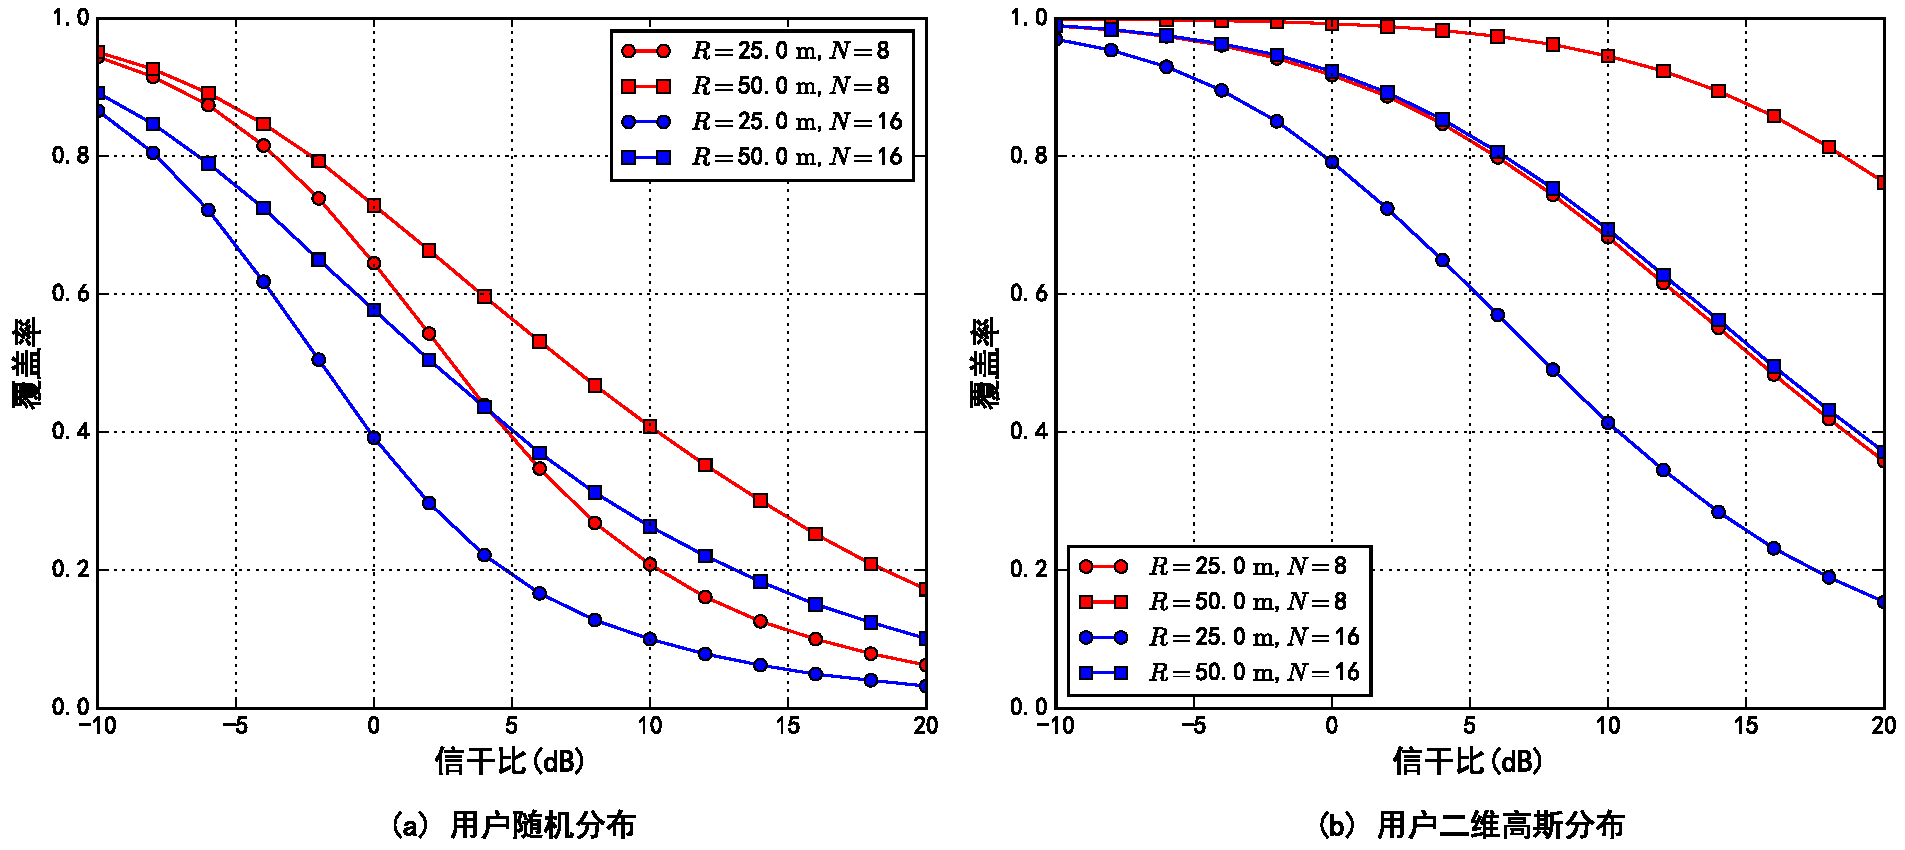
\includegraphics[width = 0.90\textwidth]{pc_random_single_circle_r_n.pdf}
\caption{环形基站部署的覆盖率性能曲线}\vspace{-0.5em}
\label{pc_random_single_circle_r_n}
\end{figure}

图~\ref{pc_random_single_circle_r_n}~给出了特定的~$N$~和~$R$~的情况下的覆盖率与信干比的关系曲线,
从曲线中,我们可以看出当~$N=8, ~12$~和~$R=25.0,~50.0\mathrm{m}$~下,网络的覆盖率的具体情况,
但曲线并不能反应覆盖率随~$N$~和~$R$~的变化的关系。
为了得到覆盖率与~$N$~和~$R$~的关系,
选定信干比的典型值~$0\mathrm{dB}$,$3\mathrm{dB}$,$5\mathrm{dB}$时,
可以得到覆盖率与~$R$~和~$N$~的关系的曲面图,
仿真的参数表如表~\ref{pc_random_single_circle_r_n_table}~所示:

\begin{table}[htbp]
\caption{覆盖率与~$R$~和~$N$~的关系的仿真参数}
\label{pc_random_single_circle_r_n_table}
\vspace{0.5em}\centering\wuhao
\begin{tabular}{cccc}
\toprule[1.5pt]
参量 & & & 设置 \\
\midrule[0.5pt]
区域~$\mathcal{D}$~的大小  & & & ~$100\mathrm{m} \times 100 \mathrm{m}$ \\
信道的类型 & & &  瑞利衰落信道\\
基站的个数~$N$~ & & &  $2\sim20$\\
圆环的半径~$R$~ & & &  $1.0\sim 50\mathrm{m}$\\
信干比门限~$\delta$~  & & & ~$0\mathrm{dB}$,$3\mathrm{dB}$,$5\mathrm{dB}$\\
用户的分布~$\Psi$~ & & & 随机分布,二维高斯分布\\
二维高斯分布的标准差~$\sigma$~ & & & ${5\mathrm{m}}$\\
信道衰落系数~$\alpha$~  & & & 4.0\\
\bottomrule[1.5pt]
\end{tabular}
\end{table}

仿真得到的曲面图如图~\ref{pc_random_single_circle_r_n_face}~所示,
可以看到当用户的分布为随机分布的情况下,覆盖率随着基站数的变化大体上是逐渐降低的,
与之前讨论得到的结果是一致的,但随着半径的变化不再是单调的,说明覆盖率的性能随着部署半径的增大先增大后减小,
最优的部署半径的值大概为~$R = 40~\mathrm{m}$~左右。
当用户的分布服从混合二维高斯分布的情况下,覆盖率随着基站数目~$N$~越多,部署基站的半径~$R$~越小,则覆盖率的性能越差,
且二者的对覆盖率的影响程度基本相同,与之前分析的结果是一致的。
在实际的部署中,可以根据覆盖率的需求合理的设定信干比门限,在设定了信干比门限的情况下,
通过图~\ref{pc_random_single_circle_r_n_face}~即可得到环形基站部署方法下使覆盖率性能达到最优的基站数~$N$~
和部署半径~$R$。
\begin{figure}[htbp]
\centering
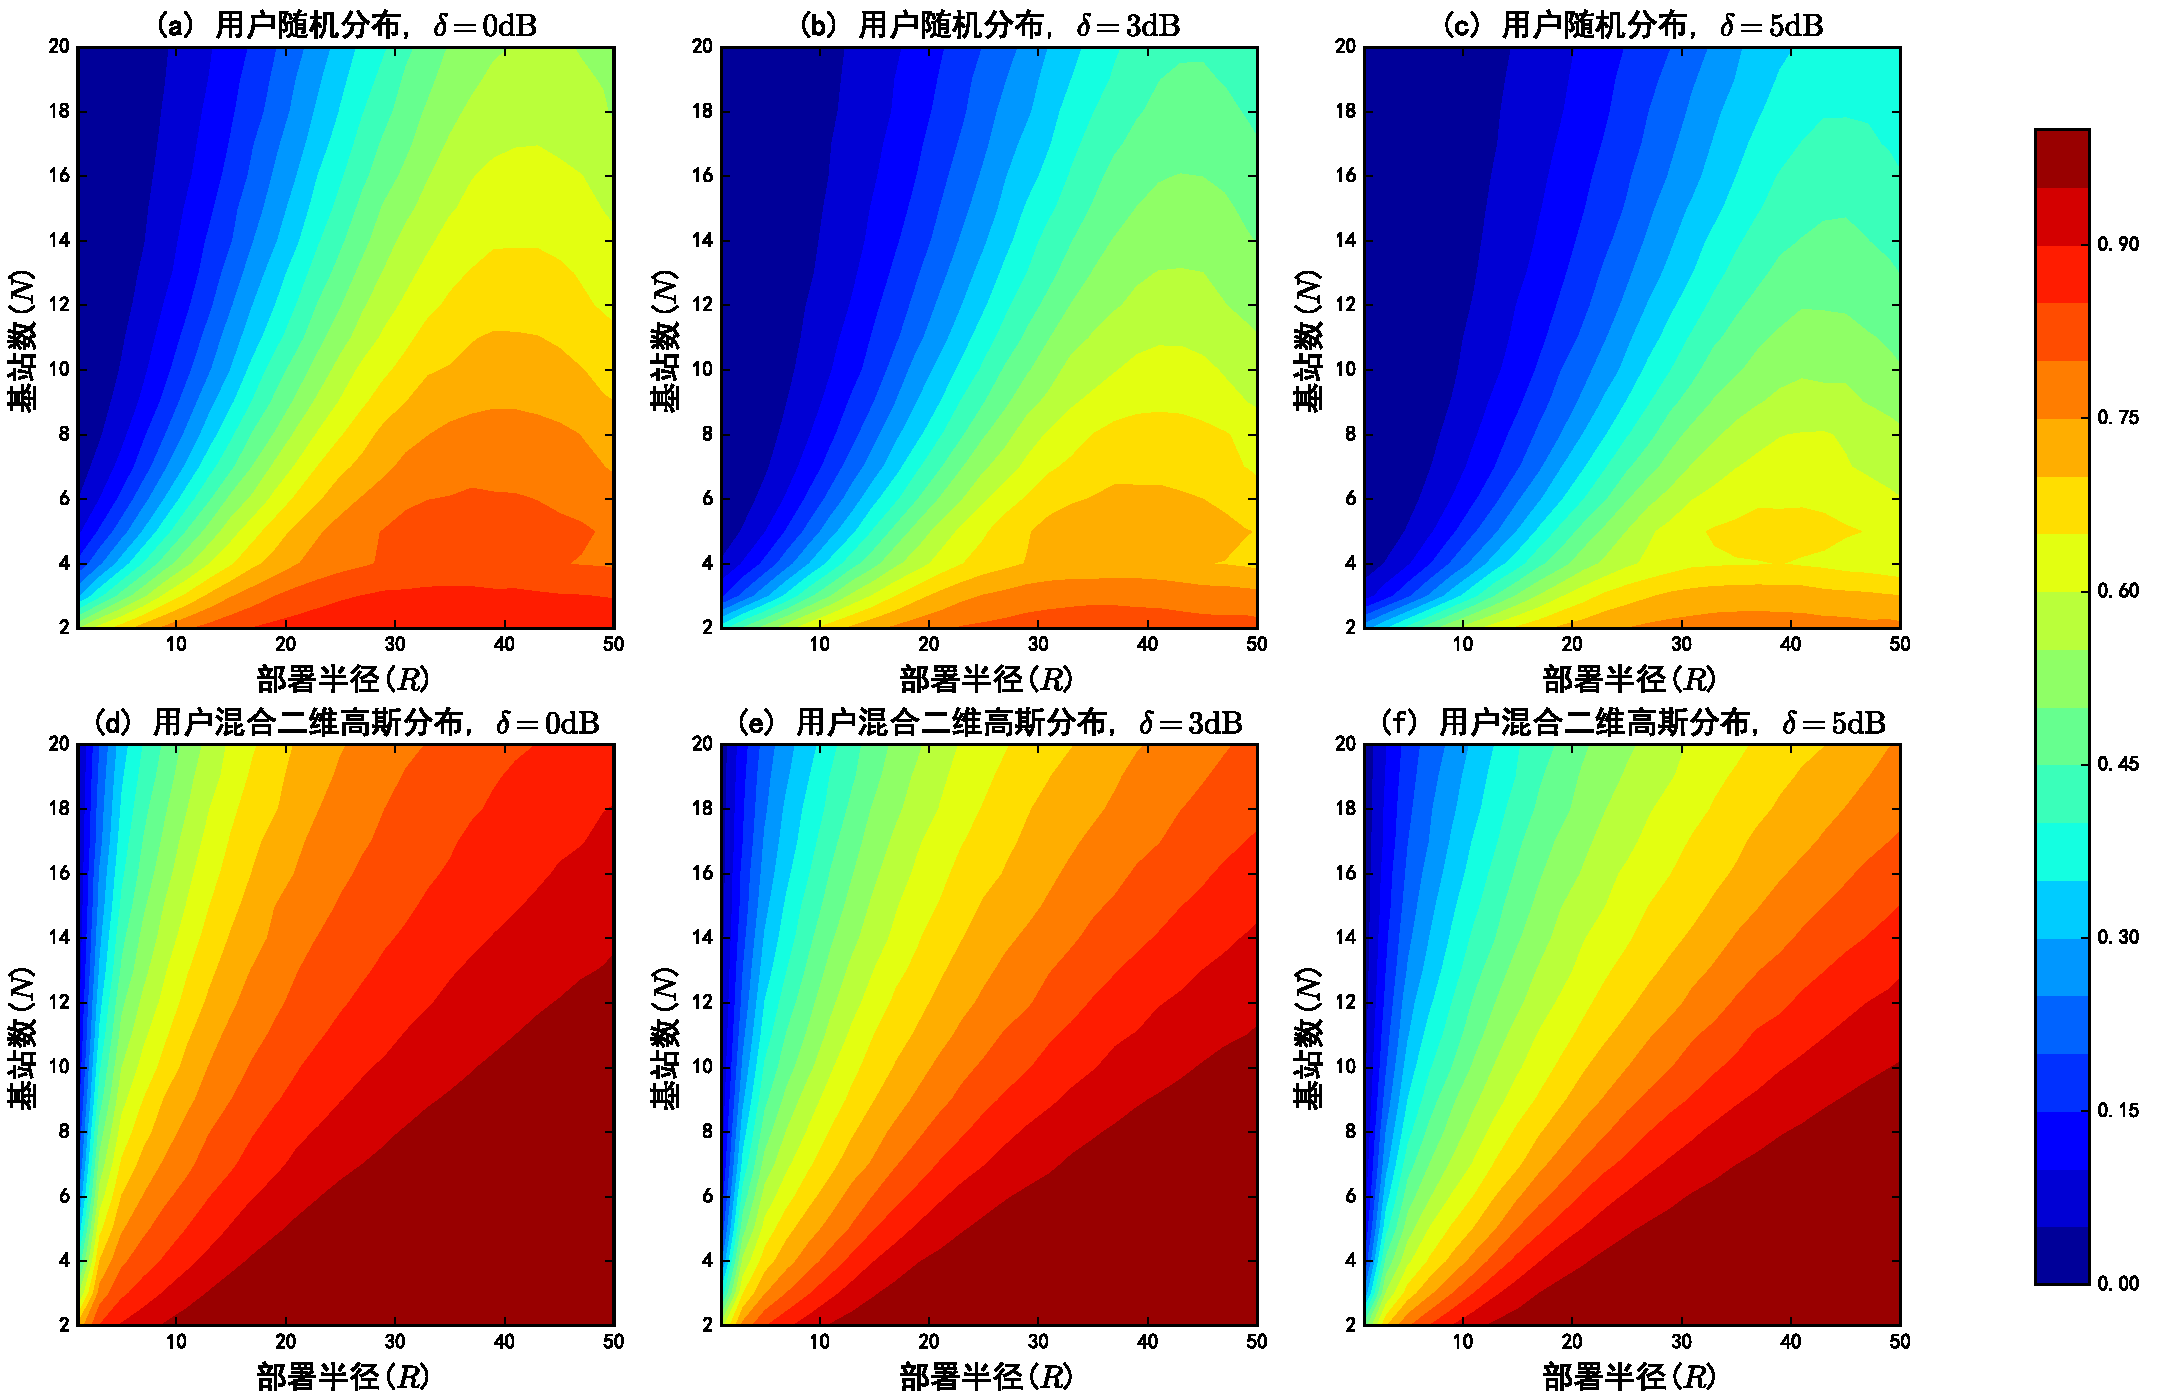
\includegraphics[width = 0.98\textwidth]{pc_random_single_circle_r_n_face.pdf}
\caption{环形基站部署的覆盖率受基站数和部署半径的影响}\vspace{-0.5em}
\label{pc_random_single_circle_r_n_face}
\end{figure}


\BiSection{方格形的基站部署的覆盖率的性能分析}{Defination of UDNs}
\BiSubsection{方格形的基站部署的拓扑结构}{Defination of UDNs}
方格形的基站部署将基站部署在固定的方格点上,部署的方法为首先在区域内的纵向每隔~$l_1$~画一条直线,
然后在横向每隔~$l_2$~画一条之间,将基站部署在直线的相交点上。
方格形的基站部署方法的示意图如图~\ref{grid_bs_station_show}~所示,
\begin{figure}[htbp]
\centering
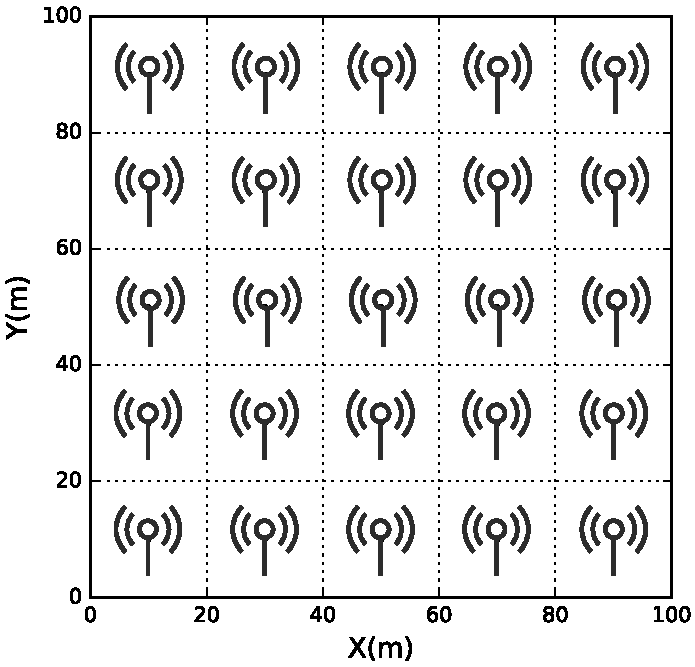
\includegraphics[width = 0.62\textwidth]{grid_bs_station_show.pdf}
\caption{方格形基站部署的拓扑结构示意图}\vspace{-0.5em}
\label{grid_bs_station_show}
\end{figure}
在图~\ref{grid_bs_station_show}~所示的基站拓扑结构中,区域~$\mathcal{D}$~为为一个~$100~\mathrm{m}\times 100~ \mathrm{m}$~的区域,
$l_1=l_2=20\mathrm{m}$,
在横向和纵向上均每隔~$20\mathrm{m}$~部署一个基站,一共在区域内共部署了~25~个基站。
再该场景下基站均匀的部署在了区域内,每个基站的负载均衡,每隔微基站覆盖的区域的性能相同,适合区域内用户均匀分布的情况。
但在未采用协作的情况下,用户选择距离其最近的基站作为服务基站,因此在小区边缘的用户受到的干扰较强,
边缘用户的覆盖率和遍历容量较差。
下面对在不同的参数条件下的基站格点形部署的性能进行定性和定量的分析。

\BiSubsection{方格形的基站部署的遍历容量}{Defination of UDNs}
对方格形基站的遍历容量分布图进行蒙特卡洛仿真分析,
仿真的参数表如表~\ref{square_grid_sinr_sim_para}~所示,
\begin{table}[htbp]
\caption{遍历容量的热力分布图的仿真参数}
\label{square_grid_sinr_sim_para}
\vspace{0.5em}\centering\wuhao
\begin{tabular}{cccc}
\toprule[1.5pt]
参量 & & & 设置 \\
\midrule[0.5pt]
区域~$\mathcal{D}$~的大小  & & & ~$100\mathrm{m} \times 100 \mathrm{m}$~ \\
横向间隔$l_1$~ & & &  ${20\mathrm{m}}$\\
纵向间隔$l_2$~ & & &  ${20\mathrm{m}}$\\
信道衰落系数~$\alpha$~  & & & 2,~4\\
\bottomrule[1.5pt]
\end{tabular}
\end{table}
对网络的各个位置,每个位置采用蒙特卡洛仿真,对每个位置的遍历容量进行仿真,
得到遍历容量的热力分布图如图~\ref{square_grid_e_capacity_show}~所示。
\begin{figure}[htbp]
\centering
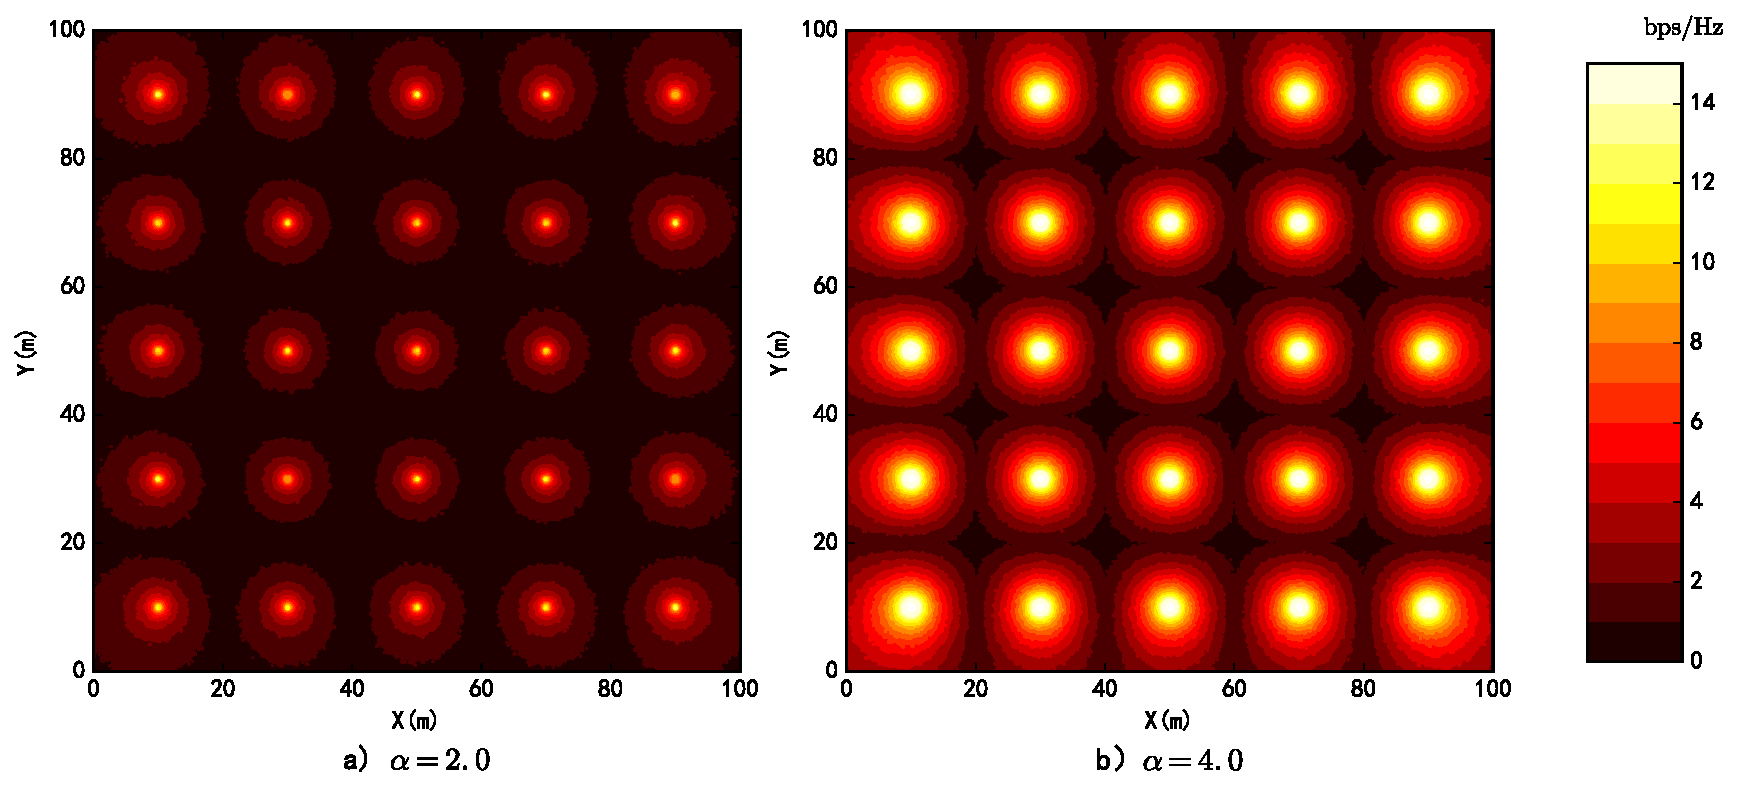
\includegraphics[width = 0.90\textwidth]{square_grid_e_capacity_show.pdf}
\caption{方格形基站部署的遍历容量热力图}\vspace{-0.5em}
\label{square_grid_e_capacity_show}
\end{figure}
可以看到较环形区域的遍历容量的热力图比较,
对于~$\alpha=2.0$~的情况,大约有超过一半的区域的遍历容量大于~$1\mathrm{bps/Hz}$,
对于~$\alpha=4.0$~的情况,大部分区域的遍历容量大于~$1\mathrm{bps/Hz}$。
与环形的基站部署的热力分布图不同,
网络中没有大面积的性能较差的区域,取而代之的是在每相互接壤的四个基站的中心处,
由于受到干扰基站的强烈的干扰,网络的遍历容量性能较差,小于~$1\mathrm{bps/Hz}$。
虽然大部分区域的覆盖率性能较好,但是仍然需要对基站中心的用户采用技术手段对其性能进行提升。

\BiSubsection{方格形的基站部署的覆盖率}{Defination of UDNs}
我们在上一小节对网络的遍历容量进行了定性的分析,
下面对网络的覆盖率性能做定量的分析,
主要分析在不同的横纵间隔~$l_1$、$l_2$~的情况下,基站的覆盖率的性能。
也对不同用户的分布情况下网络的覆盖率的性能进行了定量的分析,
考虑用户的分布~$\Psi$~分别为随机分布和混合二维高斯分布的情况。
仿真的参数表如表~\ref{square_grid_pc_sim_para}~所示,
\begin{table}[htbp]
\caption{覆盖率的仿真参数}
\label{square_grid_pc_sim_para}
\vspace{0.5em}\centering\wuhao
\begin{tabular}{cccc}
\toprule[1.5pt]
参量 & & & 设置 \\
\midrule[0.5pt]
区域~$\mathcal{D}$~的大小  & & & ~$100~\mathrm{m} \times 100 ~\mathrm{m}$ \\
基站的横向间隔~$l_1$~ & & &  $10~\mathrm{m} , 20~\mathrm{m}$ \\
基站的纵向间隔~$l_2$~ & & &  $10~\mathrm{m} , 20~\mathrm{m}$ \\
用户的分布~$\Psi$~ & & & 随机分布,二维高斯分布\\
二维高斯分布的标准差~$\sigma$~ & & & ${5\mathrm{m}}$\\
信道衰落系数~$\alpha$~  & & & 4.0\\
\bottomrule[1.5pt]
\end{tabular}
\end{table}

对所给定的横纵间隔进行组合,
对~$l_1=10~\mathrm{m},~l_2=10~\mathrm{m}$,$l_1=10~\mathrm{m},~l_2=20~\mathrm{m}$,
$l_1=10~\mathrm{m},~l_2=20~\mathrm{m}$~3~种情况进行分析,覆盖率性能的曲线如图
~\ref{pc_random_square_gird_l12}~所示,在途中可以看到,当用户的分布服从随机分布的情况下,
不同的基站的横纵间隔~$l_1$~和~$l_2$~对网络的覆盖率性能影响不大,
随着基站之间的距离逐渐边远,网络的覆盖率性能逐渐变好,
由于基站之间的距离不断地边远,干扰信号的强度更低,得到的覆盖率性能也更好,
这也可以看出随着基站密度的下降,网络的覆盖率性能提升了。
在~$l_1=l_2=10~\mathrm{m}$~的情况下,网络的~$5~\mathrm{dB}$~的覆盖率性能为~0.6。
而当用户的分布为混合二维高斯分布的情况下,
可以看到在~$l_1=l_2=10~\mathrm{m}$~时得到的曲线的覆盖率相较于其他曲线的性能有较大的提升,
因为我们假设用户分布的标准差为~$5~\mathrm{m}$,而当间隔超过~$20~\mathrm{m}$~后,
即四个标准差,网络中的用户处于边缘的概率就很小了,因此覆盖率有了显著的提升。
\begin{figure}[htbp]
\centering
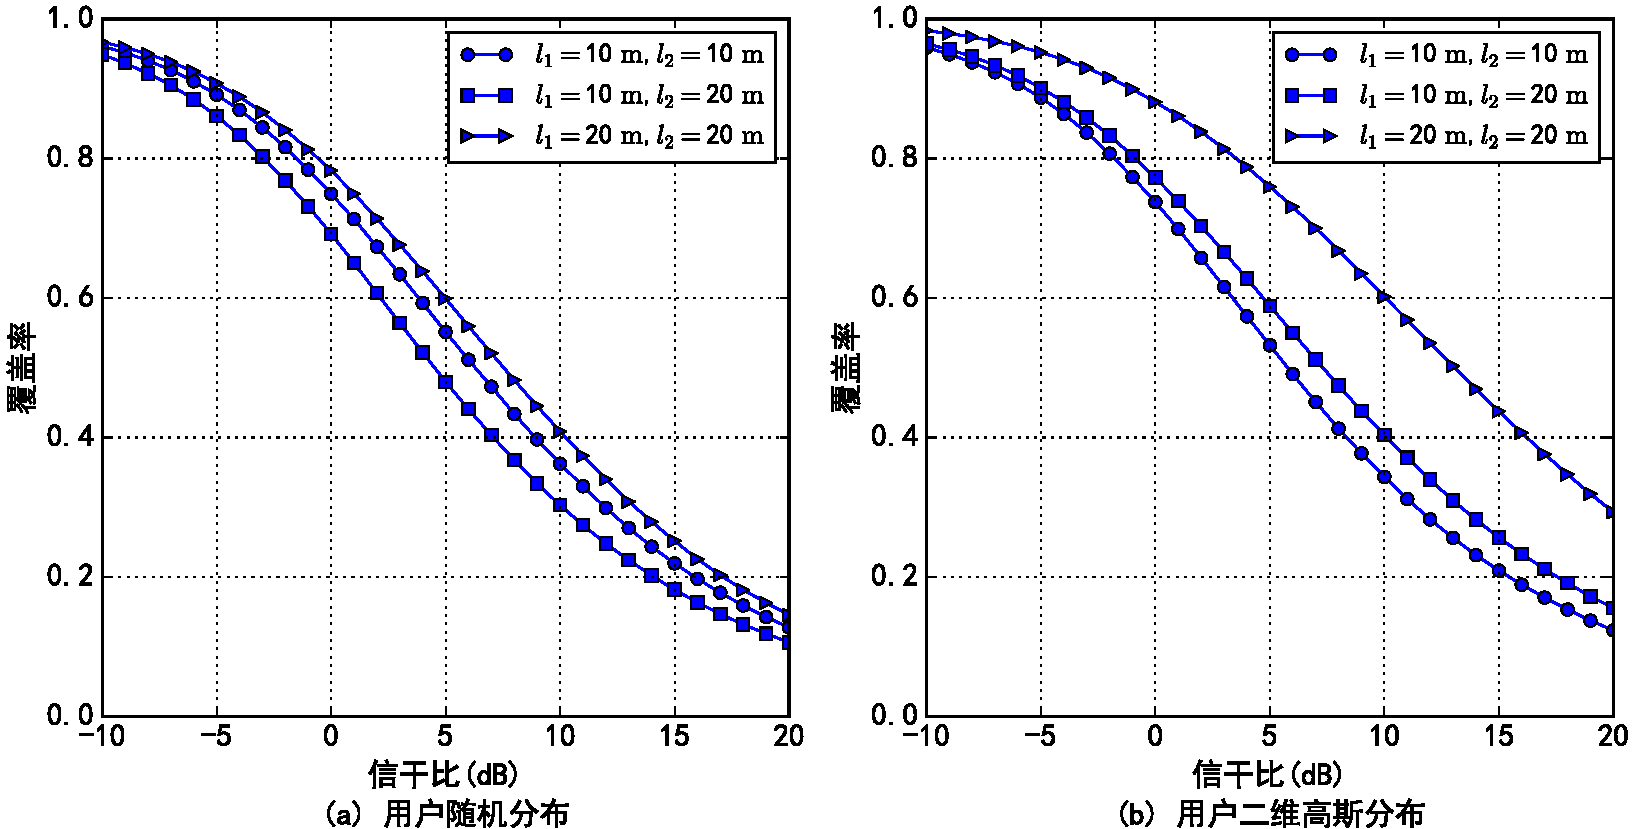
\includegraphics[width = 0.90\textwidth]{pc_random_square_gird_l12.pdf}
\caption{方格形基站部署的覆盖率性能曲线}\vspace{-0.5em}
\label{pc_random_square_gird_l12}
\end{figure}
选定信干比的值为~$0\mathrm{dB}$,$3\mathrm{dB}$~和~$5\mathrm{dB}$~时,
可以得到覆盖率与~$l_1$~和~$l_2$~的关系曲面图,仿真的参数如表~\ref{square_grid_pc_para}~所示,
\begin{table}[htbp]
\caption{覆盖率与~$l_1$~和~$l_2$~的关系的仿真参数}
\label{square_grid_pc_para}
\vspace{0.5em}\centering\wuhao
\begin{tabular}{cccc}
\toprule[1.5pt]
参量 & & & 设置 \\
\midrule[0.5pt]
区域~$\mathcal{D}$~的大小  & & & ~$100~\mathrm{m} \times 100~ \mathrm{m}$ \\
基站的横向间隔~$l_1$~ & & &  $5.0\sim 25.0\mathrm{m}$\\
圆环的纵向间隔~$l_2$~ & & &  $5.0\sim 25.0\mathrm{m}$\\
用户的分布~$\Psi$~ & & & 随机分布,二维高斯分布\\
二维高斯分布的标准差~$\sigma$~ & & & ${5\mathrm{m}}$\\
信道衰落系数~$\alpha$~  & & & 4.0\\
\bottomrule[1.5pt]
\end{tabular}
\end{table}
得到的仿真曲面图如图~\ref{pc_l1_l2}~所示,通过仿真图的结果可以看出,
在同样的基站之间的距离的情况下,
基站的的横向间距和纵向间距越是接近,其覆盖率就更高,无论是用户为随机分布还是用户为高斯分布,
均是随着距离的增加,覆盖率的性能是逐渐提高的,和之前的仿真曲线得到的分析结果基本一致。
本小节对基于方格形的基站部署方法的覆盖率性能做了仿真分析,其中通过在给定网络
的拓扑结构的情况下,对网络的覆盖率性能的定量得分析,
\begin{figure}[htbp]
\centering
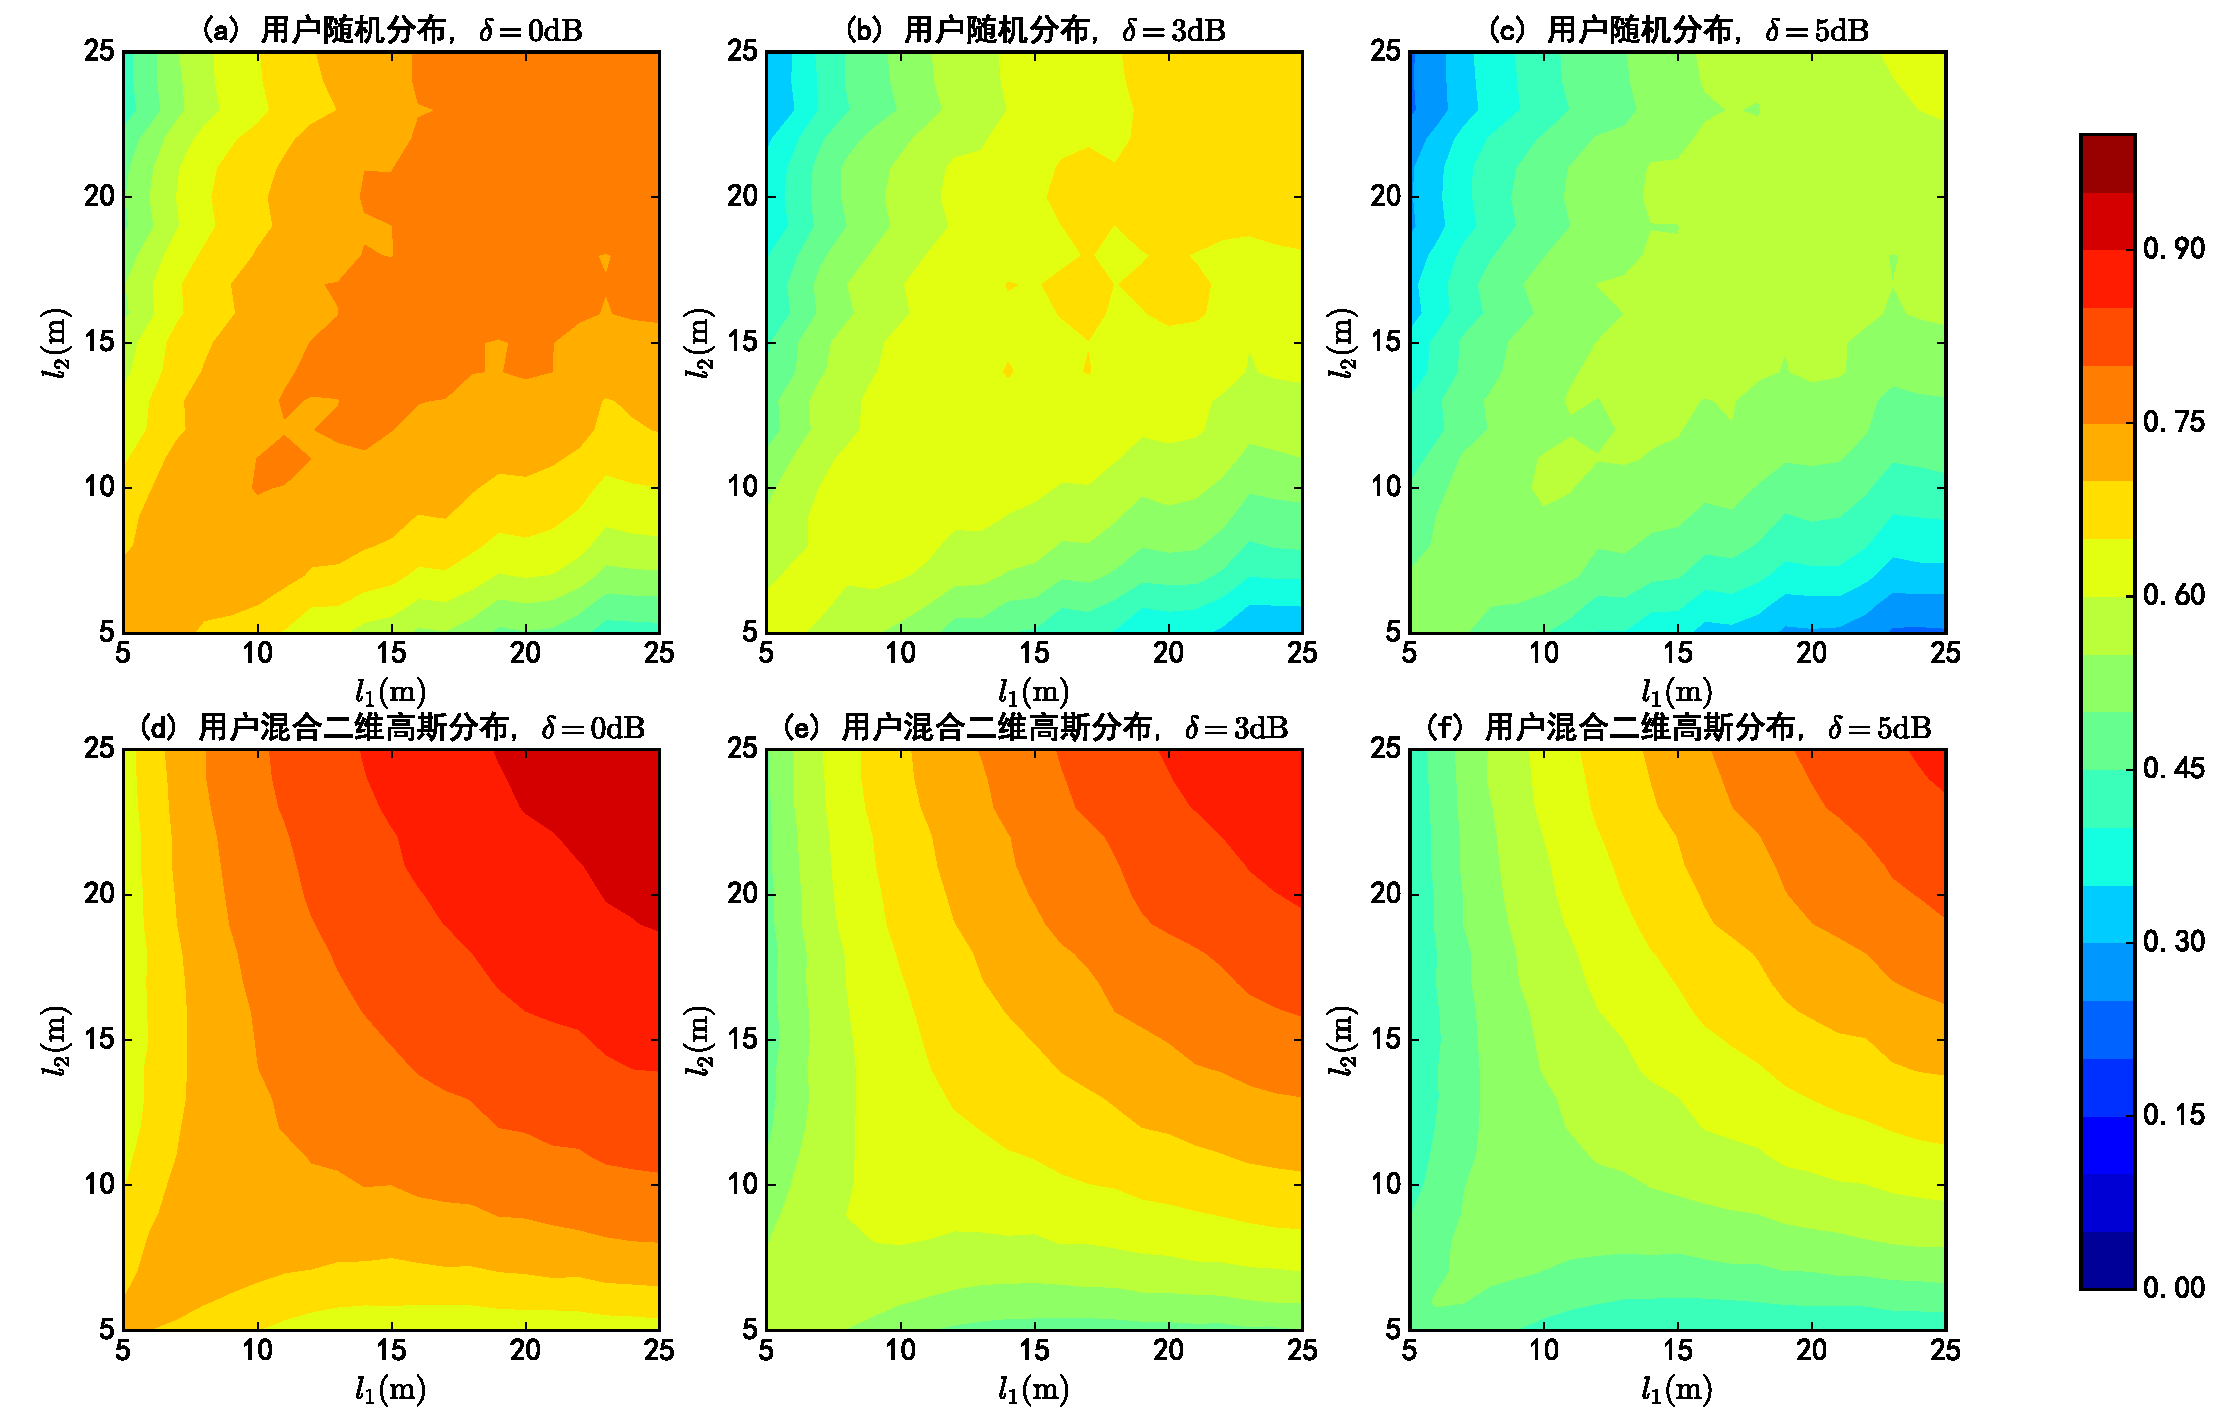
\includegraphics[width = 0.98\textwidth]{pc_l1_l2.pdf}
\caption{环形基站部署的覆盖率受基站数和部署半径的影响}\vspace{-0.5em}
\label{pc_l1_l2}
\end{figure}
可以看到覆盖率在用户为随机分布的情况下,随距离的覆盖率的提升不明显,
但当为二维高斯分布的情况下,随着距离逐渐增大,网络的覆盖率有明显的提升,
从通过颜色反映出来的图的梯度特性上可以看出,当基站之间的距离较小时,单独增加横或者纵的距离,可能会使网络的覆盖率的性能下降。
接着我们对网络中覆盖率受到基站间隔的影响进行了分析,得出当横纵间距相等时,覆盖率是距离的单调递增函数,
说明距离边远,对用户接收干扰的影响大于对用户接收有用功率的影响。

\BiSection{本章小结}{Conclusion}
本章主要介绍了网络的性能指标和基于格的基站部署的性能,
其中性能指标主要包括遍历容量,覆盖率和单位面积谱效率,
同时也对基于格的基站部署的性能进行了分析,包括环形基站的拓扑结构和方格形基站的拓扑结构。

% !Mode:: "TeX:UTF-8"

\BiChapter{密集热点区域无线网络的性能分析}{Performace Analysis}

论文的第二章已经介绍了密集热点区域无线网络的定义,根据密集热点区域无线网络的定义,我们就可以构造密集热点区域无线网络的网络模型。
构造密集热点区域无线网络的模型需要从四个方面考虑,即基站的拓扑结构,用户统计分布,信道建模与网络架构建模。在本章中,主要考虑前三个方面。

在第三章,通过对密集热点区域无线网络的系统建模,即可对密集热点区域无线网络的下行链路进行分析。通过性能分析,我们可以得到用户的信干比,网络的覆盖率,网络的单位面积频谱利用率等性能指标。

在第四章,着重考虑密集热点区域无线网络的网络架构,对密集热点区域无线网络的性能进行优化,引入提出的资源管理和调度算法,网络的覆盖率,服务用户数,单位面积频谱利用率,单位面积能量谱利用率将进一步提高。


\BiSection{密集热点区域无线网络的系统建模}{System Model}
本小节对密集热点区域无线网络进行系统建模,主要包括基站的参数与拓扑结构的分析与建模,用户的在服务区内的统计特性建模以及信道建模。
本论文主要考虑单小区,小区中配备有多个微基站。
本论文主要对下行链路的性能进行分析,即信源在基站侧,在基站中完成调制、编码发送等信号处理过程,经过信道传送至用户侧,用户在进行接收、解调、解码等过程将信息接收。
宏基站和微基站采用不同的频谱资源。
假设小区为的区域面积为~$A$。用户与发射基站建立的链路受到大尺度衰落的影响,路径损耗系数为~$\alpha$,信道噪声为加性高斯白噪声,噪声的功率为~$N$,
信道类型为瑞利信道,信道系数~$h$~服从单位指数分布,记做~$h\sim exp(1)$。$h$~的概率密度分布函数为:
\begin{equation}\label{h_pdf}
  f_H(h) = \exp(-h)
\end{equation}
概率累计分布函数为:
\begin{equation}\label{h_cdf}
  F_H(h) = \mathbb{P}[H\leq h] = 1 - \exp(-h)
\end{equation}

用户选择距离自己最近的微基站作为服务基站。
\BiSubsection{基站的参数与拓扑结构}{topology}

为了便于以后的性能分析,需要根据之前对超密集组网定义的描述,对基站的参数指标进行说明。

假设微基站的发射功率为~$P$~、每个基站配备有单根天线,小区中有多个微基站,微基站的个数为~$n$~,小区中微基站的密度为~$\lambda$~,小区密度和小区基站之间的关系如~(\ref{bs_dens_num})~所示:
\begin{equation}\label{bs_dens_num}
  n_s = \biggl\lfloor\lambda_s S\biggr\rfloor
\end{equation}
其中~$\biggl\lfloor\cdot\biggr\rfloor$~表示向下取整。所有微基站构成的集合为~$\mathcal{S}$~,第~$i$~个微基站的编号为~$S_i$~,即~$\mathcal{S}=\left\{S_1, S_2,\dots,S_{n_s}\right\}$。
微基站~$S_i$~服务的用户数为~$k_i$~个。

基站的拓扑结构即为微基站的部署方法微基站的部署则相对灵活,部署方式主要有两种,第一种为传统的格点分布,即在对微基站部署前,需要选定一种格形,如六边形格形,四边形格形等,然后将基站部署在格点上。
第二种为小区中的微基站部署是一个泊松点过程。该方法最先由~J.~ G.~ Andrews~提出\citeup{ATractable},用于刻画地物地貌对基站部署的影响。
将微基站的部署过程考虑为一个泊松点过程是更加合理的,主要有一下三个方面的原因:

(1)~ 基于格形的基站模型过于理想化

由于微基站的密度很高,容易受到外界因素的干扰。
如地形地貌的影响,如果按照格点部署,但是选定的格点周围恰好不适合部署基站,那么格点模型对该区域的刻画就不够准确,就得不到可信的性能分析。
微基站的部署也收附近的用户的统计特性的影响,如果格点周围刚好没有什么用户,显然也不会在格点上部署基站。
此时将网络中的基站建模成为格点分布也是不合理的。

(2)~ 微基站和家庭基站的部署呈现自组织性

在当前的小基站场景下,网络是密集部署的,许多微基站和家庭基站,其部署是自由部署的而不是由运营商统一部署的,这就体现了一定的随机性。
而泊松点过程就是对这种随机性的一种刻画。

(3)~ 方便对网络进行性能分析

将基站的部署看成泊松点过程,就可以应用随机几何中已经得到的很多定理简化分析过程。
通过随机几何这一数学工具,可以简化网络中的信息指标的求解,如覆盖率和单位面积频谱利用率的求解。
而基于格形的基站建模,相关性能参数的精确值只能通过蒙特卡洛仿真得到。

基站部署方式的示意图如图~\ref{bs_dis}~所示:
\begin{figure}[htbp]
\centering
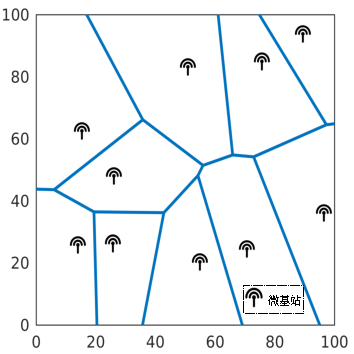
\includegraphics[width = 0.62\textwidth]{bs_dis.pdf}
\caption{基站的拓扑结构示意图}\vspace{-0.5em}
\label{bs_dis}
\end{figure}


从图~\ref{bs_dis}~是密集热点区域无线网络的基站的拓扑结构的示意图,图中,区域大小为~100$\mathrm{m}\times 100\mathrm{m}$~,模拟单个小区的情况,小区中有10个微基站,微基站的密度为~$\lambda=10^{-3}\mathrm{m}^{-2}$。
由于用户选择距离自己最近的基站进行服务,图中也采用Voronoi图对每个基站的服务区域进行了标注,即基站的服务区域为其所属的泰森多边形所占的区域。
如图中描述,微基站的部署是一个泊松点过程~$\phi$,图~\ref{bs_dis}~是泊松点过程的一次实现。
从图中也可以看出,该种基站部署方式的拓扑结构更加符合实际的情况。

当基站的部署过程为泊松点过程时,在直角坐标系下,基站的部署可以近似的看成二维随机分布,即在给定的区域内,基站在每个位置上的概率相同。
同时,根据泊松点过程的性质,已知区域的面积~$A$,那么区域内的微基站的个数~$n$~是一个随机变量,该随机变量服从与面积有关的泊松分布,泊松分布的参数为$\lambda A$。
即:
\begin{equation}
  \mathbb{P}(n_s = i) = \frac{e^{-\lambda A}(\lambda A)^{i}}{i!}
\end{equation}
根据泊松分布的性质,已知区域的面积~$A$~,微基站的密度为~$\lambda$~,则区域内的基站数量的均值为:
\begin{equation}\label{n_s_bar}
  \overline{n_s} = \lambda A
\end{equation}

\BiSubsection{用户终端的统计特性}{user distribution}

超密集组网场景是客观世界中普遍存在的一类场景。
网络区域中人物的活动规律复杂,每个人的容量需求也是十分复杂的。但我们也可以从微基站的部署以及客观实际出发,对小区中用户的统计分布做出合理的假设。

由于微基站服务于热点区域,区域内用户多,用户对容量的需求较高。因此在微基站附近的用户数量和容量需求是远高于宏基站覆盖的其他的范围的。
一般来说,微基站会部署在区域容量需求最高的地方,用户数量和容量需求随着距离微基站的距离越来越远而逐渐的变小。
根据微基站的这一特性,我们引入概率统计学中非常著名的二维混合高斯模型。二维混合高斯模型广泛的应用于人工智能,模式识别,机器学习等领域当中,用于描述事件对行为或决策的影响。
为不是一般性,此处假设二维混合高斯模型的两个维度是相互独立的。

综上所述,对于微基站~$S_i$~,用户的集合为~$\mathcal{U}_i$~,用户的个数为~$k_i$个, 用$U$表示用户的,即~$\mathcal{U}_i=\{U_1, U_2, ..., U_{k_i}\}$~微基站用户的密度为~$\mu$~。
用户围绕着基站服从二维高斯分布,二维高斯分布的方差为~$\sigma^2$。
由于泊松点过程是一个平稳的随机过程,因此可以不是一般性的假设微基站的坐标为原点,则此时,用户的概率密度分布函数即为:
\begin{equation}
  \begin{aligned}
  f_{X,Y}(x,y) &\overset{(a)}{=} f_X(x) f_Y(y) \\
               &\overset{(b)}{=} \frac{1}{\sqrt{2\pi}\sigma}\exp\left(-\frac{x^2}{2\sigma^2}\right)\cdot\frac{1}{\sqrt{2\pi}\sigma}\exp\left(-\frac{y^2}{2\sigma^2}\right) \\
               &=\frac{1}{2\pi\sigma^2}\exp\left(-\frac{x^2+y^2}{2\sigma^2}\right)
  \end{aligned}
\end{equation}

其中~$(a)$~根据随机变量的独立性,~$(b)$~为高斯分布的概率密度函数,X,Y分别为用户的横纵坐标。
用户的分布的概率密度分布函数为如图~\ref{figure_xy_pdf}~所示:
\begin{figure}[htbp]
\centering
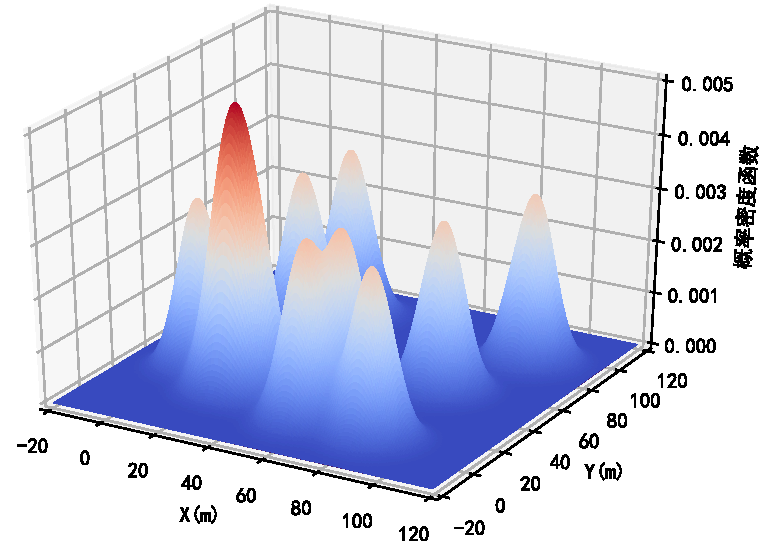
\includegraphics[width = 0.62\textwidth]{figure_xy_pdf.pdf}
\caption{微基站用户的统计分布的概率密度函数}\vspace{-0.5em}
\label{figure_xy_pdf}
\end{figure}

在图中给出了距基站~30m~内的用户的概率密度函数图,其中二维高斯分布的标准差为~10。根据高斯分布的特性,用户多集中在2个标准差范围内,即距离基站的距离为~20m~以内。

可以通过将直角坐标系转换为极坐标系,即可得到用户距基站的距离的概率密度分布函数,分布函数如式~(\ref{r_pdf})~所示:
\begin{equation}\label{r_pdf}
  f_R(r) = \frac{r}{\sigma^2}\exp(-\frac{r^2}{2\sigma^2})
\end{equation}
其中~$R$~为用户距基站的距离。

\BiSection{超密集组网的性能分析}{performance analysis}

本小节对超密集组网场景的模型进行性能分析。主要分析网络的信干噪比,网络的覆盖率以及网络的单位面积频谱利用率。覆盖率和单位面积频谱利用率的概念已在第二章中给出。

小区与用户的参数表总结如下:

\BiSubsection{小区中用户的遍历容量}{SINR}



信干噪比的定义如式~(\ref{SINR})~,可以看出信干噪比是一个与用户的接收功率,用户与服务基站建立的信道上的噪声以及收到其他微基站的干扰功率的和共同决定的。

对于微基站~$S_i$~,其所属的用户~$U_k$~的接收功率用~$P_{i,k}$~表示,如式~(\ref{P_r}):
\begin{equation}\label{P_r}
  P_{i,k} = R_{i,k}^{-\alpha} h_{i,k} P
\end{equation}
其中~$R_{i,k}$~为用户~$U_k$~距基站~$S_i$~的距离,$\alpha$~为信道衰减系数,$h_{i,k}$~是用户~$U_k$~与基站~$S_i$~构成的链路的信道系数,服从单位的指数分布,$h_{i,k}\sim exp(1)$,$P$~为基站的发射功率。
式~(\ref{P_r})~说明用户的接收功率为基站的发送功率经过大尺度衰减和小尺度衰减之后的结果。

微基站~$S_i$~中的用户~$U_k$~会受到其他基站的干扰,同样用户接收到其他基站的功率也是基站的发送功率经过大尺度衰减和小尺度衰减之后的结果,如式~(\ref{I_r})~
\begin{equation}\label{I_r}
  I_{i,k} = \sum_{\begin{subarray}{c} S_j\in \mathcal{S}\\ j \neq i\end{subarray}} R_{j,k}^{-\alpha} h_{j,k} P
\end{equation}
其中~$R_{j,k}$~为用户~$U_k$~距基站~$S_j$~的距离,$\alpha$~为信道衰减系数,$h_{j,k}$~是用户~$U_k$~与基站~$S_j$~构成的链路的信道系数,服从单位的指数分布,$h_{j,k}\sim exp(1)$,$P$~为基站的发射功率。

被微基站~$S_i$~服务的用户~$U_k$~的信干噪比的表达式即为:
\begin{equation}\label{SINR_r}
  \begin{aligned}
    \mathrm{SINR}_{i, k}&\overset{(a)}{=}\frac{P_{i,k}}{I_{i,k}+N} \\
                 &\overset{(b)}{=}\frac{R_{i,k}^{-\alpha} h_{i,k} P}{\sum\limits_{\begin{subarray}{c} S_j\in \mathcal{S}\\ j \neq i\end{subarray}} {R_{j,k}^{-\alpha} h_{j,k} P} + N}
  \end{aligned}
\end{equation}

其中$S_i\in\mathcal{S}$, $U_k\in\mathcal{U}_i$~。$(a)$~为信干噪比的定义,$(b)$~为将式~(\ref{P_r})~和~(\ref{I_r})~带入后的结果。可以看出信干噪比是一个与基站距离,基站的发射功率,噪声,信道衰减系数,信道系数有关的物理量。

由于在超密集组网的场景中,基站与用户之间的距离比较近,因此用户的接收功率在一般情况下是远远大于噪声的,即系统是一个干扰受限的系统。
因此信道的噪声可以忽略不计,忽略后即可得到用户的信干比这一物理量,如式~(\ref{SIR_r})~所示:
\begin{equation}\label{SIR_r}
  \begin{aligned}
    \mathrm{SIR}_{i, k}&\overset{(a)}{=}P_{i,k} / I_{i,k} \\
                 &\overset{(b)}{=}\frac{R_{i,k}^{-\alpha} h_{i,k}}{\sum\limits_{\begin{subarray}{c} S_j\in \mathcal{S}\\ j \neq i\end{subarray}} {R_{j,k}^{-\alpha} h_{j,k}}}
  \end{aligned}
\end{equation}
其中~$(a)$~为信干比的定义,$(b)$~为将式~(\ref{SINR_r})~中忽略噪声之后的结果。

\BiSubsection{小区中用户的覆盖率}{coverage}

覆盖率的定义式为式~(\ref{pc}),由于基站的部署是泊松点过程,泊松点过程是独立平稳的随机过程,因此可以对单个基站的覆盖率进行分析,即可的到网络的覆盖率性能。
因此,不失一般性,可以假设对基站~$S_0\in\mathcal{S}$~进行分析,定义用户距基站~$S_0$~的距离为~$r$,根据前面的分析可知,$r$~服从二维高斯分布,用户与基站~$S_0$~建立的链路的信道系数为~$h$,
$h$~服从单位指数分布,记做~$h\sim exp(1)$。

覆盖率是一个与基站的密度$\lambda$、给定的信干噪比门限~$T$~、信道的衰落系数~$\alpha$、用户的统计分布的参数~$\sigma$~有关系。
可以对式~(\ref{pc})~做进一步的推导。
\begin{equation}\label{pc_expand}
  \begin{aligned}
    p_c(T,~\lambda,~\alpha,~\sigma) &\overset{(a)}{=} \mathbb{P}[\mathrm{SINR}>T] \\
           &\overset{(b)}{=} \mathbb{E}_r[\mathrm{SINR}>T\mid r] \\
           &\overset{(c)}{=} \int_0^\infty \mathbb{P}[\mathrm{SINR}>T\mid r] \frac{r}{\sigma^2}\exp(-\frac{r^2}{2\sigma^2}) \mathrm{d} r
  \end{aligned}
\end{equation}
其中~$T$~为给定的信干噪比的门限,$\lambda$~$(a)$~为覆盖率的定义式,$(b)$~表示网络的覆盖率是一个与距离有关的量,覆盖率的值等于基站中的用户遍历所有可能出现的位置得到的覆盖率的统计平均值,$(c)$~为将式~(\ref{r_pdf})~代入后的结果。

为了得到覆盖率的表达式,需要知道当给定微基站~$S_0$~与用户的距离~$r$~以后信干噪比大于门限的概率,即$\mathbb{P}[\mathrm{SINR}>T]$。
此处假设用户距除~$S_0$~以外最近的基站的距离为~$D$~,则概率可以被拆解成为两个部分。

(1)~ 微基站~$S_0$~的用户恰好被~$S_0$~服务,即用户距基站~$S_0$~的距离~$r < D$。此时,$S_0$~为用户的服务基站,其他基站为干扰基站,即用户受到除~$S_0$~以外的其他基站的干扰。

(2)~ 微基站~$S_0$~的用户被其他的微基站进行服务,即用户距离基站~$S_0$~的距离~$r \geq D$。此时,$S_0$~为干扰基站,即用户受到~$S_0$~基站的干扰,和除服务的微基站以外的其他基站的干扰。

即根据全概率公式,总的覆盖率可以分解为

(1)~ 事件1:所观测用户的服务基站即为所属的热点的基站,且该用户能达到覆盖所需的信干噪比。

(2)~ 事件2:当所观测用户的服务基站为其他基站且该用户能达到覆盖所需的信干噪比。

这两个事件概率的加和。
根据~(1)~和~(2),可以将信干噪比大于门限的概率改写为两个部分,表达式如式~(\ref{P_SINR_2Part})~所示:
\begin{equation}\label{P_SINR_2Part}
  \begin{aligned}
  \mathbb{P}[\mathrm{SINR}>T \mid r] =& \mathbb{P}[\mathrm{SINR}>T \mid r, r < D] \mathbb{P}[r<D]\\
                               &+ \mathbb{P}[\mathrm{SINR}>T \mid r, r > D]\mathbb{P}[r>D]
  \end{aligned}
\end{equation}

对于~$r < D$~的部分,用户受到除了~$S_0$~以外的其他基站的干扰,由于超密集组网系统是一个干扰受限的系统,噪声对系统的影响相比于干扰很小,因此采用信干比,对信干噪比近似。
将信干噪比的表达式~(\ref{SIR_r})~带入到式~(\ref{P_SINR_2Part})~的前半部分,其概率的表达式如式~(\ref{P_SINR_r_le_D})~所示:
\begin{equation}\label{P_SINR_r_le_D}
  \begin{aligned}
  \mathbb{P}[\mathrm{SINR}>T \mid r, r < D] & = \mathbb{P}\left[\frac{r^{-\alpha} h}{\sum\limits_{S_j\in \mathcal{S}\backslash S_0} {R_{j,0}^{-\alpha} h_{0,k}}} > T~\bigg|~ R_{j,0} \geq D > r\right]\\
                                            & = \mathbb{P}\left[h > T r ^ \alpha \sum\limits_{S_j\in \mathcal{S}\backslash S_0} {R_{j,0}^{-\alpha} h_{j,0}}~\bigg|~ R_{j,0} \geq D > r \right]
  \end{aligned}
\end{equation}
为了简化公式,令:
\begin{equation}\label{I_define}
  I_0 = \sum\limits_{S_j\in \mathcal{S}\backslash S_0} {R_{j,0}^{-\alpha} ~ h_{j,0}}
\end{equation}
$I_0$~表示用户接收到的干扰的功率,是一个与基站部署和用户位置有关的随机变量。公式~(\ref{P_SINR_r_le_D})~可以简化为式~(\ref{P_SINR_r_le_D_simple})~:
\begin{equation}\label{P_SINR_r_le_D_simple}
  \mathbb{P}[\mathrm{SINR}>T \mid r, r < D] = \mathbb{P}\left[h > T r ^ \alpha I_0 ~\big|~ R_{j,0} \geq D > r \right]
\end{equation}
其中~$h$~是信道增益系数,是一个随机变量,该随机变量服从单位指数分布~$h \sim exp(1)$。
可以看到,在给定~$r<D$~的情况下,信干噪比大于门限~$T$~的概率可以等效为表示用户与基站~$S_0$~之间的信道系数大于~$Tr^{\alpha}I_0$~的值。
其中~$T$~为给定门限,$r$~为基站~$S_0$~与用户之间的距离,$\alpha$~为信道的损耗系数,$I_0$~为用户接收到的干扰的和的功率。

由于基站的部署是泊松点过程,因此干扰基站距离用户的距离~$R_{j,0}$~是一个随机变量,干扰基站和用户之间的信道系数~$h_{j,0}$~是一个服从单位指数分布的随机变量。
又由于干扰~$I_0$~是通过~$R_{j,0}$~和~$h_{j,0}$~这两个随机变量求得,因此信干噪比在~$r<D$~的情况下大于门限值的概率为式~(\ref{P_SINR_r_le_D_simple})~对干扰~$I_0$~求均值。
式~(\ref{P_SINR_r_le_D_simple})~可以展开为式~(\ref{P_SINR_r_le_D_simple_h}):
\begin{equation}\label{P_SINR_r_le_D_simple_h}
  \begin{aligned}
    \mathbb{P}\left[h > T r ^ \alpha I_0 ~\bigg|~ R_{j,0} \geq D > r \right] & = \mathbb{E}_{I_0}\left[\mathbb{P}\left[h > T r ^ \alpha I_0 ~\big|~ R_{j,0} \geq D > r,~ I_0 \right]\right] \\
                                                                           & \overset{(a)}{=} \mathbb{E}_{I_0}\left[\int_{T r ^{\alpha} I_0}^{\infty} \exp(-h)~\mathrm{d} h~\bigg|~ R_{j,0} \geq D > r,~ I_0\right] \\
                                                                           & = \mathbb{E}_{I_0}\left[ \exp(-Tr^\alpha I_0)~\big|~ R_{j,0} \geq D > r,~ I_0\right] \\
                                                                           & \overset{(b)}{=} \mathcal{L}_{I_0}(Tr^\alpha)
  \end{aligned}
\end{equation}
其中,(a)~为将式~(\ref{h_cdf})~带入后的结果,对~$(a)$~求积分,即可得到~$\mathbb{E}_{I}[\exp(-sI_0)]$~的形式,即随机函数~$\exp(-sI_0)$~对随机变量~$I_0$~求均值,即求随机变量~$I_0$~的聚生成函数,其求法可等效为对随机变量~$I_0$~的概率密度函数求拉普拉斯变换。
在~(b)~中,$\mathcal{L}(\cdot)$~表示拉普拉斯变换,等号右侧为拉普拉斯变换的定义式。
将式~(\ref{I_define})~带入式~(\ref{P_SINR_r_le_D_simple_h})~中,做进一步的推导,得到式~(\ref{Ls}):
\begin{equation}\label{Ls}
  \begin{aligned}
    \mathcal{L}_{I_0}(Tr^\alpha) &= \mathbb{E}_{I_0}\left[ \exp(-Tr^\alpha I_0)~\big|~ R_{j,0} \geq D > r,~ I_0\right] \\
                               &= \mathbb{E}_{\Phi, h_{j,0}}\left[\exp(-Tr^{\alpha}\sum\limits_{S_j\in \mathcal{S}\backslash S_0} {R_{j,0}^{-\alpha} ~ h_{j,0}})\right] \\
                               &\overset{(a)}{=} \mathbb{E}_{\Phi, h_{j,0}}\left[\prod\limits_{S_j\in \mathcal{S}\backslash S_0}\exp(-Tr^{\alpha} {R_{j,0}^{-\alpha} ~ h_0})\right] \\
                               &\overset{(b)}{=} \mathbb{E}_{\Phi} \left[\prod\limits_{S_j\in \mathcal{S}\backslash S_0}\frac{1}{1+ T r ^\alpha R_{j,0}^{-\alpha}}\right] \\
                               &\overset{(c)}{=} \exp\left(-2\pi\lambda_s\int_{r}^{\infty} \left(1 - \frac{1}{1+ T r ^\alpha v^{-\alpha}}\right)\mathrm{d}v\right)
  \end{aligned}
\end{equation}
其中~(a)~根据信道系数的独立同分布的特性,根据独立同分布的特性,可以将不同干扰基站的信道系数$\{h_{1,0},~h_{2,0},\dots,~h_{n,0}\}$等效为单个指数分布的随机变量~$h_0$。
(b)~为对指数分布的随机变量~$h_0$~求均值。(c)~根据泊松点过程的概率生成函数的性质,即~$\mathbb{E}\left[\prod\nolimits_{x\in\Phi}f(x)\right]=\exp(-\lambda_s\int_{~\mathbb{R}^2}(1-f(x))~\mathrm{d}x)$~。

对于式~$(\ref{P_SINR_2Part})$~中~$r > D$~的部分,因为用户选择距离自己最近的基站作为服务基站,所以基站~$S_0$~不再是用户的服务基站。
令用户距离自己最近的基站为~$S_i$,由于用户距除~$S_0$~以外最近的基站的距离为~$D$,可知~$R_{i,j}=D$。
此时用户收到来自除了干扰基站以外的其他基站的干扰如式~(\ref{I_define_r_g_d})~所示:
\begin{equation}\label{I_define_r_g_d}
I_i=\sum\limits_{ S_j\ \in\ {\mathcal{S}\ \backslash\ \{S_0,~S_i\}} }{R_{j,0}^{-\alpha} ~ h_{j,0}} + r^{-\alpha} h
\end{equation}
用户数选择~$S_i$~作为服务基站,用户的接收功率为如式~(\ref{P_define_r_g_d})~所示:
\begin{equation}\label{P_define_r_g_d}
  P_i = D^{-\alpha} h_{i,0}
\end{equation}
式~(\ref{P_SINR_2Part})~中~$r>D$~的部分,其概率的表达式如式~(\ref{P_SINR_r_ge_D_simple_h})~所示:
\begin{equation}\label{P_SINR_r_ge_D_simple_h}
  \mathbb{P}[\mathrm{SINR}>T \mid r, r < D] = \mathbb{P}\left[h_{i,j} > T D ^ \alpha I_i ~\big|~ r > D \right]
\end{equation}
与式~(\ref{P_SINR_r_le_D_simple_h})~的推导方法类似,对信道系数~$h_{i,0}$~求积分可以得到,在~$r>D$~的情况下,信干噪比大于给定门限~$T$~的概率:
\begin{equation}\label{P_SINR_r_ge_D_simple_h}
  \begin{aligned}
    \mathbb{P}\left[h_{i,j} > T r ^ \alpha I_i ~\bigg|~ r > D \right] & = \mathbb{E}_{I_i}\left[\mathbb{P}\left[h_{i,j} > T D ^ \alpha I_i ~\big|~ r > D\right]\right] \\
                                                                           & = \mathbb{E}_{I_i}\left[\int_{T D ^{\ \alpha} I_i}^{~\infty} \exp(-h_{i,j})~\mathrm{d} h_{i,j}~\bigg|~ r > D,~ I_i\right] \\
                                                                           & = \mathbb{E}_{I_i}\left[ \exp(-TD^\alpha I_i)~\big|~ r > D,~ I_i\right] \\
                                                                           & = \mathcal{L}_{I_i}(TD^\alpha)
  \end{aligned}
\end{equation}
式~(\ref{P_SINR_r_ge_D_simple_h})~说明,当~$r > D$~时,信干噪比大于给定门限的概率可以写成对干扰~$I_i$~求均值,从而可以转化成随机变量~$I_i$~的聚生成函数,
进一步的演化为对~$TD^\alpha$~求拉普拉斯变换。

将式~(\ref{I_define_r_g_d})~带入式~(\ref{P_SINR_r_ge_D_simple_h})~中,做进一步的推导,推导的方法与式~(\ref{Ls})~的推导方法类似,即首先将式~(\ref{I_define_r_g_d})带入,
再利用用户和基站之间建立的信道链路的信道系数满足独立同分布的性质,将不同的基站的信道系数等效为同一个随机变量,再将该随机变量积分,最后带入到二维泊松点过程的概率生成函数中,即可以得到式~(\ref{Ls_r_g_d})。
\begin{equation}\label{Ls_r_g_d}
  \begin{aligned}
    \mathcal{L}_{I_i}(Tr^\alpha) &= \mathbb{E}_{I_i}\left[ \exp(-Tr^\alpha I_i~\big|~ R_{j,0} \geq D > r,~ I_i\right] \\
                               &= \mathbb{E}_{\Phi, h_{j,0}}\left[\exp\left(-TD^{\alpha}(\sum\limits_{S_j\in\mathcal{S} \backslash \{S_0,~S_i\}} {R_{j,0}^{-\alpha} ~ h_{j,0}}+ r^{-\alpha} h)\right)\right] \\
                               &\overset{(a)}{=} \mathbb{E}_{\Phi, h_{j,0}}\left[\exp(-TD^{\alpha} {r^{-\alpha} ~ h})\prod\limits_{S_j\in \mathcal{S} \backslash \{S_0,~S_i\}}\exp(-TD^{\alpha} {R_{j,0}^{-\alpha} ~ h_0})\right] \\
                               &\overset{(b)}{=} \mathbb{E}_{\Phi} \left[\frac{1}{1+ T D ^\alpha r^{-\alpha}}\prod\limits_{S_j\in \mathcal{S} \backslash \{S_0,~S_i\}}\frac{1}{1+ T D ^\alpha R_{j,0}^{-\alpha}}\right] \\
                               &\overset{(c)}{=} \frac{1}{1+ T D ^\alpha r^{-\alpha}}\exp\left(-2\pi\lambda_s\frac{n}{n-1}\int_{D}^{\infty} \left(1 - \frac{1}{1+ T D ^\alpha v^{-\alpha}}\right)\mathrm{d}v\right)
  \end{aligned}
\end{equation}
其中~(a)~根据信道系数的独立同分布的特性,根据独立同分布的特性,可以将不同干扰基站的信道系数$\{h_{1,0},~h_{2,0},\dots,~h_{n,0}\}$等效为单个指数分布的随机变量~$h_0$。
(b)~为对指数分布的随机变量~$h_0$~和~$h$~分别求均值。(c)~根据泊松点过程的概率生成函数的性质,即~$\mathbb{E}\left[\prod\nolimits_{x\in\Phi}f(x)\right]=\exp(-\lambda_s\int_{~\mathbb{R}^2}(1-f(x))~\mathrm{d}x)$~。

由于~$D<r$,有~$T(\frac{D}{R})^\alpha\rightarrow 0$~并且有~$\lim\limits_{x\rightarrow 0} \frac{1}{1+x}=1$,又由于在超密集组网中,微基站的数量很多,$n$~的值很大。
因此~$\frac{n}{n-1}\rightarrow 1$~因此式~(\ref{Ls_r_g_d})~可以简化为式~(\ref{Ls_r_g_d_simple}):
\begin{equation}\label{Ls_r_g_d_simple}
    \mathcal{L}_{I_i}(Tr^\alpha) \approx \exp\left(-2\pi\lambda_s\int_{D}^{\infty} \left(1 - \frac{1}{1+ T D ^\alpha v^{-\alpha}}\right)\mathrm{d}v\right)
\end{equation}

将式~(\ref{P_SINR_r_le_D_simple_h})~和式~(\ref{P_SINR_r_ge_D_simple_h})~带入到式~(\ref{P_SINR_2Part})~中,可以得到网络中某一个点上的用户,其信干噪比大于给定门限的概率为式~(\ref{P_SINR_2Part_Ls})~:
\begin{equation}\label{P_SINR_2Part_Ls}
  \mathbb{P}[\mathrm{SINR}>T \mid r] = \mathcal{L}_{I_0}(Tr^\alpha)\mathbb{P}[r<D] + \mathcal{L}_{I_i}(TD^\alpha)\mathbb{P}[r>D]
\end{equation}
即给定用户距离微基站~$S_0$~的距离~$r$~后,用户的信干噪比~$\mathrm{SINR}$~大于预设门限的概率需要分为两个部分进行讨论。
当微基站~$S_0$~为距离用户最近的基站,即~$r < D$,用户的服务基站为~$S_0$~的情况下,用户的信干噪比~$\mathrm{SINR}$~大于预设门限的概率
和微基站~$S_0$~不是距离用户最近的基站,即~$r > D$,用户的服务基站为除~$S_0$~之外的其他基站~$S_i$的情况下,用户的信干噪比~$\mathrm{SINR}$~大于预设门限的概率。
信干噪比大于预设门限的概率可以通过对干扰求聚生成函数的值,其在形式上等于对干扰求拉普拉斯变换。

对式~(\ref{P_SINR_2Part_Ls})~做进一步的展开,将式~(\ref{Ls})~和式~(\ref{Ls_r_g_d})~的结果带入到式中,可以得到给定用户距离微基站~$S_0$~后,信干噪比大于预设门限的概率关于~$r$,$D$,$\lambda_s$,$\alpha$,$T$的函数。
如式~(\ref{P_SINR_2Part_Ls_expand})~所示:
\begin{equation}\label{P_SINR_2Part_Ls_expand}
  \begin{aligned}
  \mathbb{P}[\mathrm{SINR}>T \mid r] =& \exp\left(-2\pi\lambda_s\int_{r}^{\infty} \left(1 - \frac{1}{1+ T r ^\alpha v^{-\alpha}}\right)\mathrm{d}v\right) \mathbb{P}[r<D]\\
  & + \frac{1}{1+ T D ^\alpha r^{-\alpha}}\exp\left(-2\pi\lambda_s\frac{n}{n-1}\int_{D}^{\infty} \left(1 - \frac{1}{1+ T D ^\alpha v^{-\alpha}}\right)\mathrm{d}v\right)\mathbb{P}[r>D]
\end{aligned}\end{equation}
将式~(\ref{Ls})~和式~(\ref{Ls_r_g_d_simple})~的结果带入到式~(\ref{P_SINR_2Part_Ls})~中即可得到可以得到给定用户距离微基站~$S_0$~后,信干噪比大于预设门限的概率关于~$r$,$D$,$\lambda_s$,$\alpha$,$T$的近似函数。
\begin{equation}\label{P_SINR_2Part_Ls_expand}
  \begin{aligned}
  \mathbb{P}[\mathrm{SINR}>T \mid r] \approx & \exp\left(-2\pi\lambda_s\int_{r}^{\infty} \left(1 - \frac{1}{1+ T r ^\alpha v^{-\alpha}}\right)\mathrm{d}v\right)\mathbb{P}[r<D] \\
  & + \exp\left(-2\pi\lambda_s\int_{D}^{\infty} \left(1 - \frac{1}{1+ T r ^\alpha v^{-\alpha}}\right)\mathrm{d}v\right)\mathbb{P}[r>D]
\end{aligned}\end{equation}

根据\cite{ATractable}中的结果,对等式的两个部分分别做变量替换~$u=\left(\frac{v}{rT^{\frac{1}{\alpha}}}\right)$
和$u=\left(\frac{v}{DT^{\frac{1}{\alpha}}}\right)$,可以得到式~(\ref{P_SINR_2Part_Ls_expand})~的更精简的表达,如式~(\ref{P_SINR_2Part_Ls_expand_simple})~所示:
\begin{equation}\label{P_SINR_2Part_Ls_expand_simple}
  \begin{aligned}
  \mathbb{P}[\mathrm{SINR}>T \mid r] &= \exp\left(-\pi r^2\lambda_s\  \rho(T,\alpha)  \right)\mathbb{P}[r<D] \\
     &\quad + \frac{1}{1+ T D ^\alpha r^{-\alpha}} \exp\left(-\pi D ^2 \lambda_s\ \frac{n}{n-1} \rho(T,\alpha)\right)\mathbb{P}[r>D]\\
    &\approx  e^{-\pi r^2\lambda_s\  \rho(T,\alpha)  }\mathbb{P}[r<D]
    + e^{-\pi D ^2 \lambda_s\ \rho(T,\alpha)}\mathbb{P}[r>D]
\end{aligned}\end{equation}
其中,
\begin{equation}\label{rho}
  \rho(T,\alpha) = T ^{1/\alpha} \int_{T^{-2/\alpha}}^{\infty} \frac{1}{1+u^{\alpha/2}}\mathrm{d}u
\end{equation}

将式~(\ref{P_SINR_2Part_Ls_expand_simple})~带入到式~(\ref{pc_expand})~中,并对变量~$r$,$D$~积分,即可得到覆盖率最后的表达式~(\ref{pc_expand_rd_int}):
\begin{equation}\label{pc_expand_rd_int}
  \begin{aligned}
    &\quad\ p_c(T,~\lambda,~\alpha,~\sigma) \\
    &\overset{(a)}{=}\int_0^\infty  \int_D^{\infty}   \exp\left(-\pi r^2\lambda_s\  \rho(T,\alpha)  \right) f(D)    \mathrm{d} D f(r) \mathrm{d} r\\
    & \qquad + \int_0^\infty  \int_D^{\infty}   \frac{1}{1+ T D ^\alpha r^{-\alpha}} \exp\left(-\pi D ^2 \lambda_s\ \frac{n}{n-1} \rho(T,\alpha)\right) f(D)    \mathrm{d} D f(r) \mathrm{d} r\\
    &\overset{(b)}{\approx} \int_0^\infty  \int_D^{\infty}   \exp\left(-\pi r^2\lambda_s\  \rho(T,\alpha)  \right) f(D)    \mathrm{d} D f(r) \mathrm{d} r\\
    & \qquad + \int_0^\infty  \int_D^{\infty}   \exp\left(-\pi D ^2 \lambda_s\ \rho(T,\alpha)\right) f(D)    \mathrm{d} D f(r) \mathrm{d} r
  \end{aligned}
\end{equation}
其中,
\begin{equation}
  f(D) = e^{-\lambda_s}\pi D^2 2 \pi \lambda_s D
\end{equation}
\begin{equation}
  f(r) = \frac{r}{\sigma^2}\exp(-\frac{r^2}{2\sigma^2})
\end{equation}
分别为用户距离最近的基站和距离和微基站~$S_0$~距离最近的基站~$S_i$~的距离的概率密度分布函数。
(a)为覆盖率~$p_c(T,~\lambda,~\alpha,~\sigma)$~的表达式,(b)~是根据式~(\ref{P_SINR_2Part_Ls_expand_simple})~进行合理近似后的简化的表达式。

对于~(b),对等式的右边求积分,可以得到更加简化的结果,如式~(\ref{pc_expand_rd_int_expand_simple}):
\begin{equation}\label{pc_expand_rd_int_expand_simple}
p_c(T,~\lambda,~\alpha,~\sigma) = \frac{1}{1+\rho(T,\alpha)} + \frac{\rho(T,\alpha)}{1+\rho(T,\alpha)}\cdot\frac{1}{2\pi\sigma^2\lambda_s(1+\rho(T,\alpha))+1}
\end{equation}
$\rho(T,\alpha)$~的定义式为式~(\ref{rho})。
$T$~为给定的信干噪比的门限,$\lambda_s$为服务区域内基站的密度。$\alpha$~为信道衰落系数。$\sigma$~为用户围绕热点分布的标准差的参数。
等式的前半部分与\cite{ATractable}给出的公式相同,为当用户的分布为随机分布时的覆盖率。
通过前面的分析推导,可以得到定理~\ref{pc_theorem}:
\begin{theorem}\label{pc_theorem}
  在二维的自由空间中,微基站的部署是泊松点过程~$\Phi$~,微基站的密度为~$\lambda_s$,基站的个数为~$n$~。
  用户的分布服从以其所围绕的基站的坐标为均值,$\sigma^2$为方差的二维高斯分布。
  用户选择距离其最近的基站作为服务基站,其他的基站作为干扰基站。
  则网络的覆盖率为:
  \begin{equation}
    \begin{aligned}\label{pc_expand_rd_int_expand_complex}
    &p_c(T,~\lambda,~\alpha,~\sigma)\\
    &{=}\int_0^\infty  \int_D^{\infty}   \exp\left(-\pi r^2\lambda_s\  \rho(T,\alpha)  \right) f(D)    \mathrm{d} D f(r) \mathrm{d} r\\
    & \quad + \int_0^\infty  \int_D^{\infty}   \frac{1}{1+ T D ^\alpha r^{-\alpha}} \exp\left(-\pi D ^2 \lambda_s\ \frac{n}{n-1} \rho(T,\alpha)\right) f(D)    \mathrm{d} D f(r) \mathrm{d} r\\
    \end{aligned}
  \end{equation}
  其中,
  \begin{equation}
    f(D) = e^{-\lambda_s}\pi D^2 2 \pi \lambda_s D
  \end{equation}
  \begin{equation}
    f(r) = \frac{r}{\sigma^2}\exp(-\frac{r^2}{2\sigma^2})
  \end{equation}
  分别为用户距离最近的基站和距离和微基站~$S_0$~距离最近的基站~$S_i$~的距离的概率密度分布函数。
  \begin{equation}\label{rho}
    \rho(T,\alpha) = T ^{1/\alpha} \int_{T^{-2/\alpha}}^{\infty} \frac{1}{1+u^{\alpha/2}}\mathrm{d}u
  \end{equation}
  可对~$p_c$~进行合理的近似,得到渐进的上界,近似的表达式为:
  \begin{equation}\label{pc_expand_rd_int_expand_simple}
  p_c(T,~\lambda,~\alpha,~\sigma) = \frac{1}{1+\rho(T,\alpha)} + \frac{\rho(T,\alpha)}{1+\rho(T,\alpha)}\cdot\frac{1}{2\pi\sigma^2\lambda_s(1+\rho(T,\alpha))+1}
  \end{equation}
\end{theorem}

可以看到,该场景下的区域覆盖率主要与微基站用户分布的方差,基站的密度,信道的路径损耗因数有关系。

(1) ~当用户覆盖所需的信干比较小的时候,第一项起主导的作用,当用户覆盖所需的信干比较大的时候,第二项起主导作用。
在覆盖所需的信干比较大的时候,覆盖率与密度成反比,与用户分布的方差成反比。

(2) ~覆盖率随着热点区域的密度的增加而减少。
当基站的密度趋于无穷大的情况下,小区的覆盖率将近似等于在小区中用户服从随机分布的情况的覆盖率。如式~(\ref{lambda_to_infty})~:
\begin{equation}\label{lambda_to_infty}
  \lim_{\lambda_s \rightarrow \infty} p_c(T,\lambda_s,\alpha,\sigma) = \frac{1}{1+\rho(T, \alpha)}
\end{equation}
(3) ~覆盖率随着用户分布的方差的增大而减少,
当表示用户分散程度的用户分布的方差趋于无穷大的情况下,
小区的覆盖率将近似等于在小区中用户服从随机分布的情况的覆盖率。
如式~(\ref{sigma_to_infty})~:
\begin{equation}\label{sigma_to_infty}
  \lim_{\sigma \rightarrow \infty} p_c(T,\lambda_s,\alpha,\sigma) = \frac{1}{1+\rho(T, \alpha)}
\end{equation}

覆盖率是评定无线网络性能的一个重要的概念,并且根据覆盖率,可以很容易的得到有能达到给定的速率要求在整个区域中的所有用户的占比。
同时该物理量也是单位区域上信干噪比的概率分布函数的补函数。

\BiSubsection{小区中用户的单位面积频谱效率}{coverage}
考虑到不同区域上的频谱效率相差可能非常悬殊,因此在密集热点的网络环境下,
频谱效率将不能够完全反映整个区域的无线网络的性能,取而代之的是单位面积谱效率这一物理量,其定义为在单位面积上的频谱效率,其数学表达式为:
\begin{equation}\label{ASE_3}
  \eta_{ASE}=C/(B\cdot S) = \lambda_s\mathbb{E}[\log_2(1+\mathrm{SINR})]
\end{equation}
求取的方法和覆盖率的求取方法基本相同。根据公式:
\begin{equation}\label{E_to_int_P}
\mathbb{E}(X)=\int_{t>0}\mathbb{P}(X>t)dt
\end{equation}
将式~(\ref{ASE_3})~中的均值用式~(\ref{E_to_int_P})~进行替换,得到公式~(\ref{ASE_pc}):
\begin{equation}\label{ASE_pc}
  \begin{aligned}
  \eta_{ASE} &= \lambda_s\int_{t>0} \mathbb{P}[\log_2(1 + \mathrm{SINR}) > t] \mathrm{d} t \\
             &= \lambda_s\int_{t>0} \mathbb{P}[\mathrm{SINR} > 2 ^ {t}-1] \mathrm{d} t \\
             &= \lambda_s\int_{t>0} p_c(2^{t}-1,\lambda_s,\alpha,\sigma) \mathrm{d} t \\
  \end{aligned}
\end{equation}
带入公式~(\ref{pc_expand_rd_int_expand_simple}),即可得到定理~\ref{ASE}:
\begin{theorem}\label{ASE}
  在二维的自由空间中,微基站的部署是泊松点过程~$\Phi$~,微基站的密度为~$\lambda_s$,基站的个数为~$n$~。
  用户的分布服从以其所围绕的基站的坐标为均值,$\sigma^2$为方差的二维高斯分布。
  用户选择距离其最近的基站作为服务基站,其他的基站作为干扰基站。
  则网络的单位面积频谱效率~$\eta_{ASE}$~为:
  \begin{equation}\label{ASE_pc_expand}
    \begin{aligned}
    \eta_{ASE} =& \lambda_s\int_{t>0} \frac{1}{1+\rho(2 ^ {t}-1,\alpha)} \\
                &+ \frac{\rho(2 ^ {t}-1,\alpha)}{1+\rho(2 ^ {t}-1,\alpha)}\cdot\frac{1}{2\pi\sigma^2\lambda_s(1+\rho(2 ^ {t}-1,\alpha))+1}  \mathrm{d} t
    \end{aligned}
  \end{equation}
\end{theorem}

可以看出,随着方差逐渐增大,场景的区域面积谱效率越来越接近均匀分布的场景。
在热点场景下,区域面积谱效率首先随着基站密度的增加迅速增加,之后随着基站密度的增加区域面积谱效率呈现线性的增加。

\BiSection{密集热点区域无线网络性能的仿真分析}{System Model}
基于前两节的阐述和分析,这一节对密集热点区域无线网络的系统性能应用~Python3.5~进行仿真分析,对第二小节得到的结果给出理论曲线和仿真曲线,
对性能分析的结果进行验证与定性定量的分析。具体的仿真参数如表~\ref{pc_sim_para}~所示。
\begin{table}[htbp]
\caption{密集热点区域无线网络的仿真参数设定}
\label{pc_sim_para}
\vspace{0.5em}\centering\wuhao
\begin{tabular}{cccc}
\toprule[1.5pt]
参量 & & & 设置 \\
\midrule[0.5pt]
基站的分布 & & & 泊松点过程 \\
用户的分布  & & & 混合二维高斯分布\\
区域的大小  & & & ~$100\mathrm{m} \times 100 \mathrm{m}$~ \\
微基站的天线数 & & & 1 \\
基站的发射功率 & & & 1 $\mathrm{W}$ \\
用户的天线数 & & & 1 \\
上行/下行 & & & 下行 \\
服务基站的选择方式 & & & 就近原则 \\
是否有联合传输 & & & 否\\
$\mathrm{SINR}$ & & & $-10 \sim 20$~dB \\
\bottomrule[1.5pt]
\end{tabular}
\end{table}
\BiSubsection{对网络遍历容量性能的仿真分析}{Time diversity}
由于用户的接收信干噪比是一个和用户在网络中的位置和用户与基站建立的信道链路的信道系数有关系,
下面针对泊松点过程的基站,对基站中的每个位置的遍历容量进行定性的分析,附加的仿真参数如表~\ref{sinr_sim_para}~所示:
\begin{table}[htbp]
\caption{网络中的遍历容量的仿真参数设定}
\label{sinr_sim_para}
\vspace{0.5em}\centering\wuhao
\begin{tabular}{cccc}
\toprule[1.5pt]
参量 & & & 设置 \\
\midrule[0.5pt]
基站的个数~$n$~ & & &  100\\
基站的密度~$\lambda_s$~ & & &  0.01/${\mathrm{m}^2}$\\
信道衰落系数~$\alpha$~  & & & 2,~4\\
\bottomrule[1.5pt]
\end{tabular}
\end{table}

根据公式~(\ref{SIR_r}),在干扰受限信道的情况下,用户的接收信干噪比近似等于用户的接收信干比,
接收信干比与信道的衰减系数~$\alpha$,用户距离服务基站和干扰基站的距离,链路的信道系数共同决定。
由于场景为平稳的瑞利信道,因此可以通过遍历容量去反映在网络中的不同位置上用户的信干噪比性能。
在区域内,各个位置的遍历容量示意图如图~\ref{network_show}~所示。
\begin{figure}[htbp]\label{network_show}
\centering
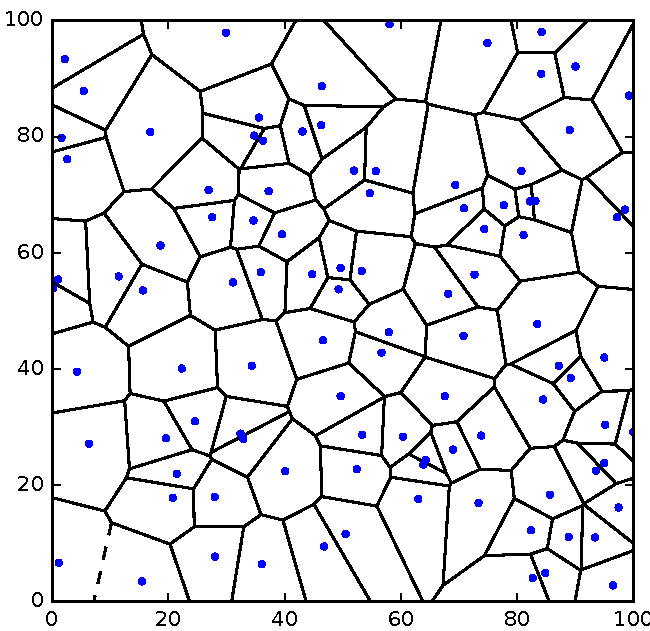
\includegraphics[width = 0.62\textwidth]{bs_station.pdf}
\caption{网络的拓扑示意图}\vspace{-0.5em}
\label{bs_dis}
\end{figure}
给定了泊松点过程的一次实现,既可以确定网络的遍历容量,遍历容量的表达式如~(\ref{e_capacity_formular})。
网络的遍历容量的示意图如图~\ref{e_capacity_show}~所示。
\begin{figure}[htbp]\label{network_show}
\centering
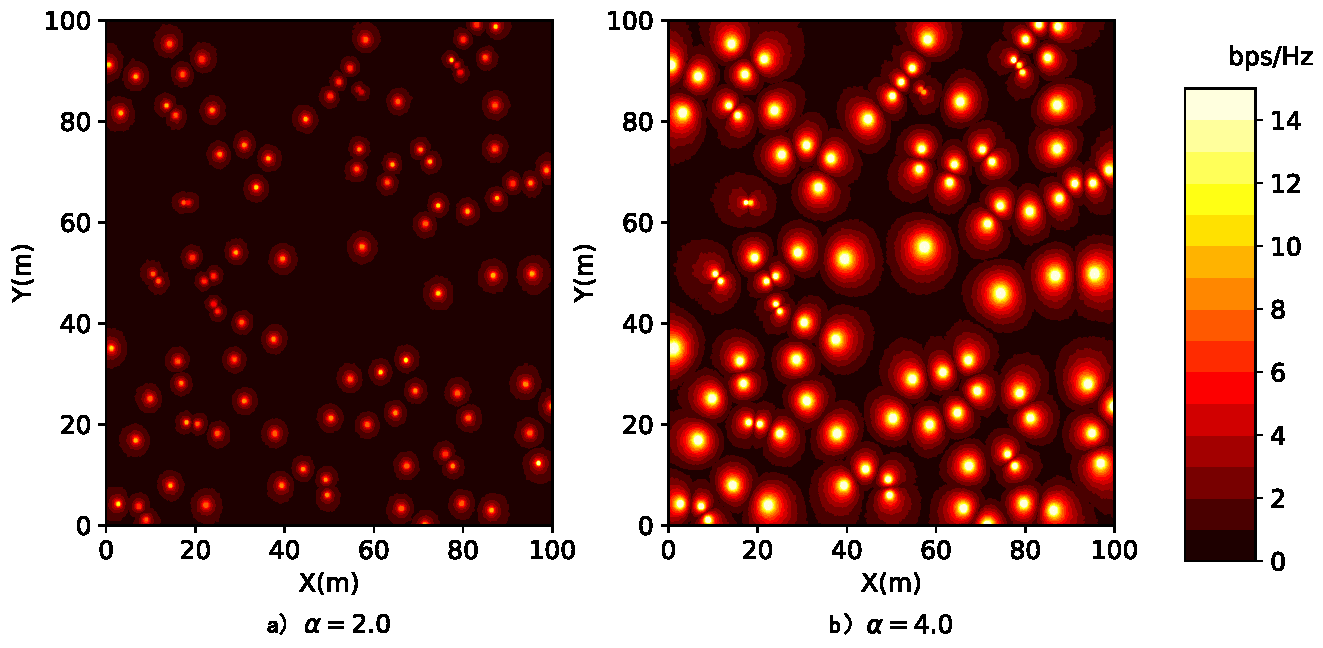
\includegraphics[width = 0.98\textwidth]{e_capacity_hotmap.pdf}
\caption{网络中每个位置的遍历容量示意图:~(左)~$\alpha=2$~(右)~$\alpha=4$}\vspace{-0.5em}
\label{e_capacity_show}
\end{figure}
图~\ref{e_capacity_show}~显示了当~$\alpha=2$~和当~$\alpha=4$~的情况下,
网络中各个位置的遍历容量,其中遍历容量是一个与网络中的接收信干噪比直接有关的一个量。
因此也可以大体上反应区域内接收信噪比的分布,接收信噪比和网络中不同位置的遍历容量共同反应了网络的有效性。
信道的衰减系数~$\alpha$~反应了网络的大尺度衰减的效果的强弱,仿真所选取的~$\alpha$~是两个典型值,当~$\alpha=2$~时,反应了自由空间中的网络的情况,
当~$\alpha=4$~时,反应了在城市环境中的网络的大尺度衰减的效果。
$\alpha$~越大,随着用户距离基站的距离逐渐边缘,用户的接收功率下降越快。
导致了用户的接收到的有用信号的功率是降低的,但是与此同时,由于~$\alpha$~的增大也使得用户接收到干扰基站功率也会变小,
因此,给定了用户的位置,用户的遍历容量随着信道衰减系数~$\alpha$~的变化需要做进一步的讨论。

从图~\ref{e_capacity_show}~中可以很清楚的看出,
在~$\alpha=4$~的情况下的网络中的遍历容量是好于在~$\alpha=2$~的情况下网络的遍历容量的。这也说明了信道系数~$\alpha$~对干扰功率的影响大于对
接收功率的影响,导致了随着~$\alpha$~的增大,网络的遍历容量性能更好。在~$\alpha = 2$~的情况下,区域内的遍历容量~$C_{Rayleigh}<2~bps/\mathrm{Hz}$~占区域面积的50\%以上,
而当~$\alpha = 2$~时,区域内的遍历容量~$C_{Rayleigh}<2~bps/\mathrm{Hz}$~占整个区域的面积大于50\%,且处在大多数的微基站的中心区域的用户的遍历容量大于~$C_{Rayleigh} > 14~bps/\mathrm{Hz}$。

\BiSubsection{对网络覆盖率性能的仿真分析}{Time diversity}
本小节将对网络的覆盖率性能进行仿真分析,根据定理~$\ref{pc_theorem}$~得到了网络中的覆盖率的表达式,其中式~(\ref{pc_expand_rd_int_expand_complex})~为准确的表达式,
~(\ref{pc_expand_rd_int_expand_simple})~为近似的表达式。从表达式中我们可以看出,可以看到,该场景下的区域覆盖率主要与微基站用户分布的方差,基站的密度,信道的路径损耗因数有关系。
下面将分别针对不同的微基站的密度,不同的路径损耗因数,用户分布的不均匀程度分别对网络的覆盖率性能进行分析。

\textbf{(1)}~不同的信道衰减系数对网络的覆盖率性能的影响
根据式~(\ref{pc_expand_rd_int_expand_complex})~和式~(\ref{pc_expand_rd_int_expand_simple}),
随着小区的信道衰减系数的增加,覆盖率逐渐增加。
对不同的微基站的密度对网络的覆盖率性能的影响的仿真参数如表~\ref{pc_alpha_sim_para}~所示:

\begin{table}[htbp]
\caption{衰减系数对覆盖率性能影响的仿真参数}
\label{pc_alpha_sim_para}
\vspace{0.5em}\centering\wuhao
\begin{tabular}{cccc}
\toprule[1.5pt]
参量 & & & 设置 \\
\midrule[0.5pt]
基站的个数~$n$~ & & &  100\\
基站的密度~$\lambda_s$~ & & &  0.01/${\mathrm{m}^2}$\\
信道衰落系数~$\alpha$~  & & &  2,~4\\
用户的分散程度~$\sigma$~ & & & 5.0~$\mathrm{m}$ \\
仿真点数 & & & $10^{4}$ \\
\bottomrule[1.5pt]
\end{tabular}
\end{table}

对公式~(\ref{pc_expand_rd_int_expand_simple})进行数值分析,给出数值曲线。
并对如表中给出的参数所构成的网络进行蒙特卡洛仿真,得到区域中网络的仿真曲线,将得到的结果作比较,
对不同信道衰减系数下的网络的覆盖率性能进行了比较。曲线图如图~\ref{pc_alpha_graph}~所示:

\begin{figure}[htbp]\label{pc_alpha_graph}
\centering
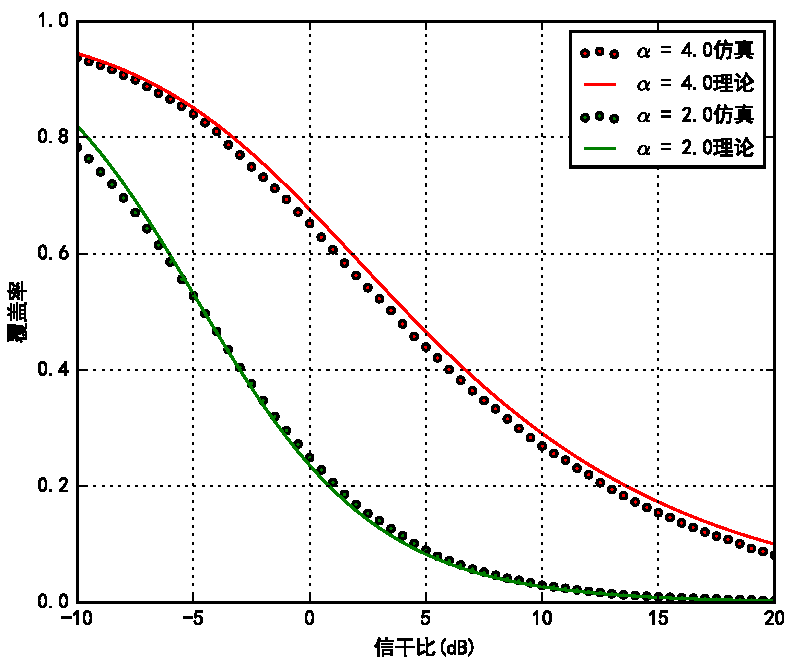
\includegraphics[width = 0.62\textwidth]{pc_alpha.pdf}
\caption{不同衰减系数下的网络覆盖率性能的比较}\vspace{-0.5em}
\label{e_capacity_show}
\end{figure}
从图中可以看出,推导出的覆盖率的近似表达式,与网络通过仿真得到的覆盖率的情况吻合较好。
这验证了推导出的结果的正确性。
也可以看到,由于随着信道的衰减系数的增加,信道衰减系数对干扰的影响相较于对接收有用信号功率的影响更明显,
因此随着信道的衰减系数的增加,网络的覆盖率的性能逐渐的变好,这与推导出的覆盖率的公式所反应出的性质是一致的。
这也表明,在城市区域内,由于衰减系数较大,增加网络的密集度以换取高的网络的性能的可行性。

\textbf{(2)}~不同的微基站的密度对网络的覆盖率性能的影响

根据式~(\ref{pc_expand_rd_int_expand_complex})~和式~(\ref{pc_expand_rd_int_expand_simple}),
随着小区的微基站的密度的增加,覆盖率逐渐降低,随着基站密度的增加,基站的密度对覆盖率的影响将越来越小。
对不同的微基站的密度对网络的覆盖率性能的影响的仿真参数如表~\ref{pc_lambda_s_sim_para}~所示:

\begin{table}[htbp]
\caption{信道衰减系数对覆盖率性能的影响的仿真参数}
\label{pc_lambda_s_sim_para}
\vspace{0.5em}\centering\wuhao
\begin{tabular}{cccc}
\toprule[1.5pt]
参量 & & & 设置 \\
\midrule[0.5pt]
基站的个数~$n$~ & & &  25,50,100\\
基站的密度~$\lambda_s$~ & & &  0.0025/${\mathrm{m}^2}$,0.005/${\mathrm{m}^2}$, 0.01/${\mathrm{m}^2}$\\
信道衰落系数~$\alpha$~  & & &  4\\
用户的分散程度~$\sigma$~ & & & 5.0~$\mathrm{m}$ \\
仿真点数 & & & $10^{4}$ \\
\bottomrule[1.5pt]
\end{tabular}
\end{table}

对公式~(\ref{pc_expand_rd_int_expand_simple})进行数值分析,给出数值曲线。
并对如表中给出的参数所构成的网络进行蒙特卡洛仿真,得到区域中网络的仿真曲线,将得到的结果作比较。
并且对不同基站密度下的网络的覆盖率性能进行了比较。
曲线图如图~\ref{pc_lambda_s_graph}~所示:
\begin{figure}[htbp]
\centering
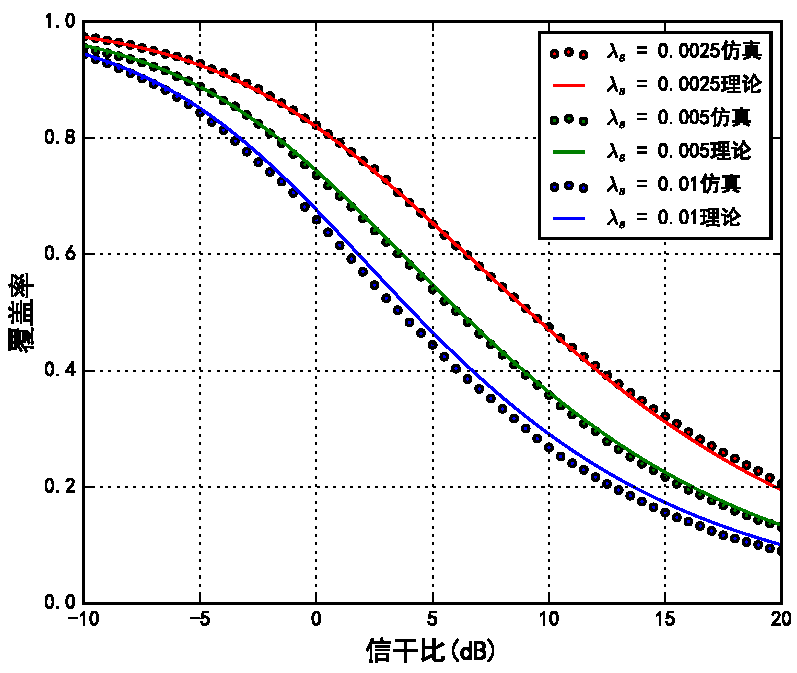
\includegraphics[width = 0.62\textwidth]{pc_lambda_s.pdf}
\caption{不同微基站密度下的网络覆盖率性能的比较}\vspace{-0.5em}
\label{pc_lambda_s_graph}
\end{figure}
从图中可以看出,推导出的覆盖率的近似表达式,与网络实际的覆盖率的情况吻合较好,推导出的近似式是与真实情况很接近的上界,在图中也得到了体现。
这验证了推导出的结果的正确性。
也可以看到,由于随着微基站的密度的增加,处在边缘区域的用户的数量逐渐增多,因此随着微基站的密度的增加,网络的覆盖率的性能逐渐的变差。
从图中可以看出,当基站的密度为~$0.01\mathrm{m}^{-2}$~时,
约有~$66\%$~的用户的信干比超过~$0\mathrm{dB}$,
约有~$44.5\%$~的用户的信干比超过~$5\mathrm{dB}$。

通过图中的结果也可以说明,在不采用任何算法进行干扰管理的情况下,网络中的中断概率较高,
网络的整体性能较差,
不能满足超密集组网场景下的高接入量,低终断概率的要求,因此在基站密度较高的情况下,需要采用干扰管理算法进行干扰协调。

\textbf{(3)}~不同的用户的离散程度对网络的覆盖率性能的影响

根据式~(\ref{pc_expand_rd_int_expand_complex})~和式~(\ref{pc_expand_rd_int_expand_simple}),
随着微基站的用户的离散程度的增加,覆盖率逐渐降低,随着基站密度的增加,基站的密度对覆盖率的影响将越来越小。
对不同的微基站的密度对网络的覆盖率性能的影响的仿真参数如表~\ref{pc_sigma_sim_para}~所示:

\begin{table}[htbp]
\caption{用户离散程度对覆盖率性能的影响的仿真参数}
\label{pc_sigma_sim_para}
\vspace{0.5em}\centering\wuhao
\begin{tabular}{cccc}
\toprule[1.5pt]
参量 & & & 设置 \\
\midrule[0.5pt]
基站的个数~$n$~ & & &  100\\
基站的密度~$\lambda_s$~ & & &  0.01/${\mathrm{m}^2}$\\
信道衰落系数~$\alpha$~  & & &  4\\
用户的分散程度~$\sigma$~ & & & 5.0~$\mathrm{m}$,10.0~$\mathrm{m}$, $\infty$  \\
仿真点数 & & & $10^{4}$ \\
\bottomrule[1.5pt]
\end{tabular}
\end{table}
其中用户的分散程度为~$\infty$~表示用户的分布服从均匀分布。

对公式~(\ref{pc_expand_rd_int_expand_simple})进行数值分析,给出数值曲线。
并对如表中给出的参数所构成的网络进行蒙特卡洛仿真,得到区域中网络的仿真曲线,将得到的结果作比较。
并且对不同用户的离散程度下的网络的覆盖率性能进行了比较, 并且对当用户服从均匀分布的情况下的覆盖率的性能,以及仿真结果进行了比较。

曲线图如图~\ref{pc_sigma_graph}~所示:
\begin{figure}[htbp]
\centering
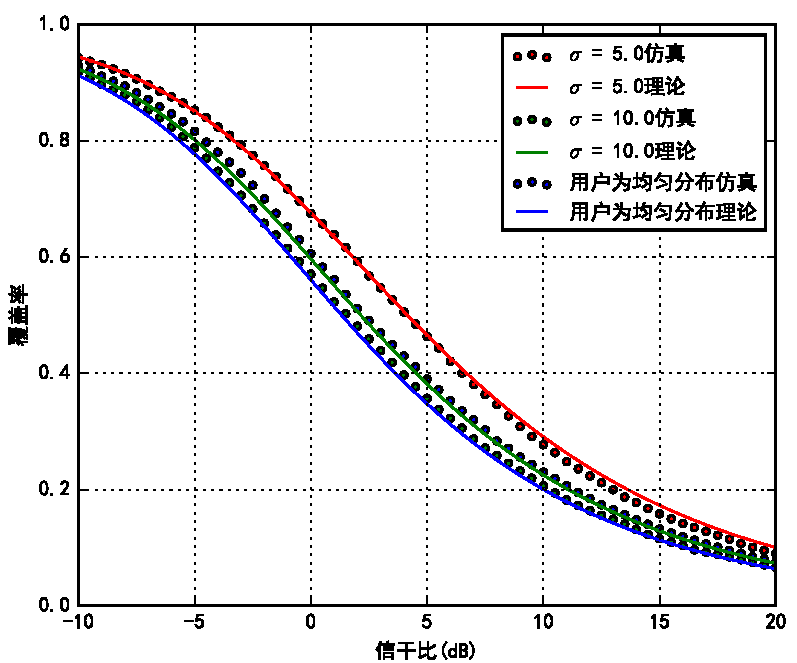
\includegraphics[width = 0.62\textwidth]{pc_sigma.pdf}
\caption{不同用户分散程度下的网络覆盖率性能的比较}\vspace{-0.5em}
\label{pc_sigma_graph}
\end{figure}

可以看到,由于随着用户的分散程度增加,处在边缘区域的用户的数量逐渐增多,因此用户分散程度的增加,网络的覆盖率的性能逐渐的变差。
并且从图中也可以看出,随着用户的分散程度的逐渐增加,网络的覆盖率的性能逐渐趋于均匀分布的情况。
从图中可以看出,当用户的分散程度~$\sigma=5.0$~时,
用户的信干比超过~$0\mathrm{dB}$的概率较均匀分布的情况高~$10\%$~左右,
用户的信干比超过~$5\mathrm{dB}$的概率较均匀分布的情况高~$13\%$~左右。
也可以看出,式~(\ref{pc_expand_rd_int_expand_simple})~更好的反映出了用户在分布不均匀的情况下的覆盖率性能。
由于微基站多布放在用户量大的热点区域,微基站也就是为了热点区域服务的,因此微基站附近的用户多于区域的其他位置是合理的。
在这种情况下,式~(\ref{pc_expand_rd_int_expand_simple})~得到的结果更能反应这种特性。


\BiSubsection{对网络的单位面积谱效率的数值分析}{ASE}

本小节考虑在不同的用户的分散程度的情况下,区域的单位面积谱效率随着微基站部署的密度的增加的变化情况,对其性能进行数值分析,
式~(\ref{ASE_pc})~为小区中单位面积频谱效率的表达式,可以看到单位面积频谱效率是一个与基站密度,小区中用户的发散程度都有关的量,
小区中的单位面积频谱效率随小区微基站密度的变化曲线图如图~\ref{ASE_lambda_sigma}~所示:
\begin{figure}[htbp]
\centering
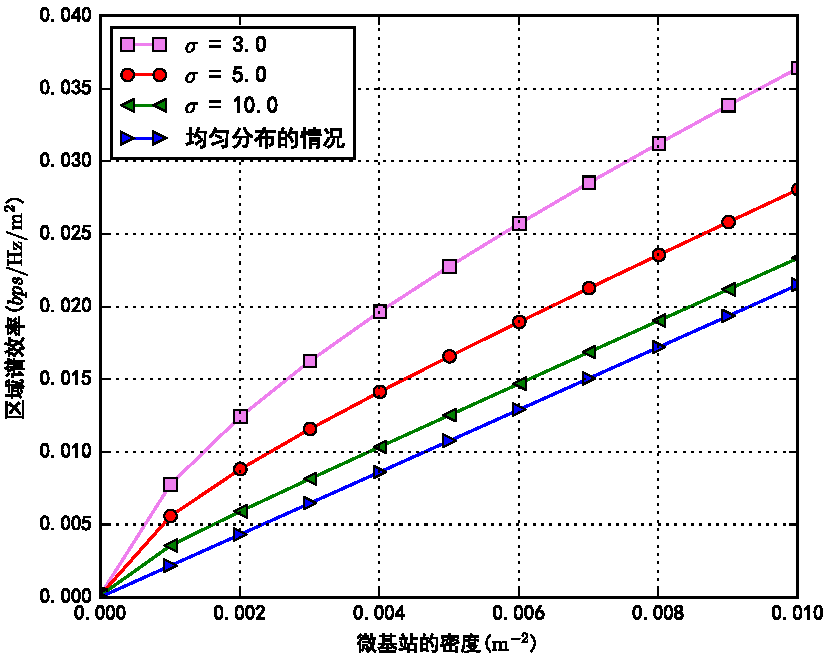
\includegraphics[width = 0.62\textwidth]{ase_sigma_lambda.pdf}
\caption{小区的单位面积谱效率与基站密度的关系}\vspace{-0.5em}
\label{ASE_lambda_sigma}
\end{figure}

从图~\ref{ASE_lambda_sigma}~中可以看出,
小区网络的单位面积频谱效率随着微基站的密度的增加而逐渐的增加,
增长速度逐渐降低最后趋于平稳,呈现随着微基站密度的增加而线性增加。
区域面积频谱效率也和用户的发散程度有关系,发散程度越小,则单位面积频谱效率就越大,
并且随着为基站密度的增长速度越晚的趋于平稳。
这与式~(\ref{ASE_pc})~中所反映的性质是一致的。


\BiSection{本章小结}{Conclusion}
本章主要对密集热点区域无线网络的网络性能进行了分析。

首先,给出了密集热点区域无线网络的网络模型,
给出了基于泊松点过程的基站网络拓扑结构。
引入用户的发散程度~$\sigma$~来表示用户在区域中的不均匀性,更好的反应了热点区域相较于小区其他区域的用户量,容量需求量更大这一特点。

接着给出了小区中用户的接收信干噪比的表达式,对网络的覆盖率,单位面积频谱效率性能进行了理论分析。

最后,通过对小区的遍历容量,覆盖率和单位面积频谱效率进行了仿真,并验证了理论分析的正确性,
对小区的性能进行了定性定量的分析,讨论了微基站的密度、小区中用户的分散程度、信道的衰落系数对网络性能的影响。

% !Mode:: "TeX:UTF-8"

\BiChapter{密集热点区域无线网络的优化}{UDN optimization}

根据第三章的分析,在不采用任何干扰管理和协调算法的情况下,网络中能达到正常工作的信干噪比的用户占总共的用户量的百分比很低。
从而导致了反应网络中所有用户有效性的平均的性能的单位面积谱效率也很低。
因此需要设计一种干扰管理和协调算法提升网络的性能。

本章分两步解决干扰管理的问题,第一步对小区中的微基站进行分簇,从而使边缘用户减少,
第二步对每个簇中的基站采用~CRAN~网络架构进行联合,由于~CRAN~架构可以将不同微基站的基带信号传输至云化的~BBU~池进行统筹处理。
在~BBU~池侧,可以采用联合传输预编码的方法将发送给不同用户的信息在空域上相互正交,从而达到干扰消除的目的。
\BiSection{密集热点区域无线网络的干扰管理算法的架构}{algorithm construction}
根据图~\ref{e_capacity_show}~显示的结果,在小区中心的用户,受到的干扰较小,遍历容量较好,能达到正常通信的遍历容量需求。
小区边缘的用户的遍历容量较差,反应了小区边缘受到的干扰较为强烈,
接收信干噪比较低,处于边缘的终端出现中断的概率很大,因此要想办法去让边缘用户的性能提升,从而降低网络的中断概率,提高网络覆盖率。

联合传输技术是伴随第四代移动通信~(4G)~提出的一个关键技术。其主要的思想是以用户为中心,将基站联合起来,进行协作,共同对用户进行服务。
由于基站间相互联合共同服务区域内的用户,
处在基站边缘的用户的干扰功率也能被用户利用成为有用的接收功率,从而使得边缘用户的有效性大大提升。
联合传输中,网络由用于处理数字信号的BBU池,用户传输信号的微基站和前向回程链路组成。
传送给用户的信息首先通过BBU池进行数据处理,在通过前向回程链路传输到基站端,由于采用了干扰消除算法,因此基站传送给用户的信息均为用户可以利用的有效信号,
实现基站联合传输共同服务区域内的用户的目的。

在第三章中,定义了网络的网络中基站的拓扑结构,用户的统计特性,信道的基本模型。
即在面积为~$A$~的区域中,基站的分布~$\Phi$~是一次泊松点过程的实现,
其密度参数为~$\lambda_s$,基站的个数为~n~个,用户在网络中的分布在微基站附近的分布更多,
随着距离基站越来越远,用户出现的概率越小。
假设用户服从以基站位置为均值的混合二维高斯分布,物理量~$\sigma$~表示用户的发散程度。
在之前的分析中,由于没有采用多用户联合传输技术,因此所有基站的功率假设是等功率的,
而采用了联合传输以后,可以对所有的基站进行统一的调度,因此网络可以进一步通过功率控制的方法进行优化。
现假设基站~$S_i$~的最大发射功率为~$P$。
除此之外,本文采用的多用户联合传输中,为了进行干扰管理,采用预编码的技术进行干扰消除,预编码矩阵为~$\mathbf{W}$。
用户~$U_j$~接收到基站~$S_i$~的接收功率受到基站~$S_i$~的最大的发射功率~$P$,预编码矩阵~$\mathbf{W}$,描述信道的大尺度衰落的信道衰减系数~$\alpha$,
描述瑞利信道的随机变量~$h$决定。

 假设采用~BPSK~调制方式,在小区中一共有~$k$~个用户~$n$~个基站,
 基站发射给用户的信息为~$\mathbf{q}=\{q_1,q_2,\dots,q_j,\dots,q_k\}$,
 其中~$q_j\in\{1,-1\}$~表示用户~$U_j$~想要接收到的信号。
 在进行预编码之前需要首先要确定每个用户所需要分配的功率。
 在进行功率分配后,待发射的信号~$\mathbf{x} = \{x_1,x_2,\dots,x_j,\dots,x_k\} = \{p_1 q_1,p_2 q_2,\dots,p_j q_j,\dots,p_k q_k\}$。
 其中为~$\mathbf{p}=\{p_1,p_2,\dots,p_j,\dots,p_k\}$~为功率分配权重。
 因此用户~$j$~分配到的功率的值为~${p_j}^2$~

 预编码矩阵为~${\mathbf{W}=\{w_{ij}\}}_{n\times k}$。
 其中~$w_{ij}$~表示第~$j$~个用户所发送的信息在第~$i$~个基站所占的权值。则基站的发射信号向量~$\mathbf{s}$可表示为:
 \begin{equation}\label{send_s}
   \mathbf{s}=\mathbf{W} \mathbf{x}
 \end{equation}
其中~$\mathbf{x}$~为发射信号的向量,$\mathbf{W}$~为预编码矩阵,
可将预编码矩阵~$\mathbf{W}$~表示为~$n\times 1$~的分块矩阵
~$\mathbf{W}=\{\mathbf{w}_1, \mathbf{w}_2,\cdots,\mathbf{w}_k\}^{\mathrm{T}}$。
在联合传输的过程中,所有的基站共享用户的发送信息和信道状态信息,
以得到状态信息作为参数,得到的预编码矩阵,即可以对网络的有效性进行优化,
通过预编码矩阵修改发送每个用户信息的权重,
将加权后的信号交由基站进行发送。

基站发送的信号受到大尺度衰落和小尺度衰落的影响。
定义系数矩阵~$\mathbf{G}=\{g_{ij}\}_{k\times n}$,
其中~$g_{ij}\in\mathbb{R}$,$g_{ij} = h_{ij}R_{ij}^{-\alpha}$,
其中~$h_{ij}$~和~$R_{ij}$~分别表示基站~$S_i$~和用户~$U_j$~之间的信道系数和距离。
用户的接收信号向量~$\mathbf{y}$~为:
\begin{equation}\label{received_y}
  \mathbf{y} = \mathbf{Gs} + \mathbf{z}
\end{equation}
其中~$\mathbf{G}$~为信道的系数矩阵,$z\in \mathbb{R}$~为加性高斯白噪声的功率。

若采用基于~ZFBF~的多用户联合传输技术,则预编码矩阵~$\mathbf{W}$~为:
\begin{equation}\label{precode_w}
  \mathbf{W} = \mathbf{G}^{\mathrm{T}}(\mathbf{G}\mathbf{G}^{\mathrm{T}})^{-1}
\end{equation}
其中~$\mathrm{T}$~表示转置,即采用基于~ZFBF~的多用户联合传输技术的情况下,
预编码矩阵为信道系数矩阵的广义逆。

将式~(\ref{send_s})~和式~(\ref{precode_w})~带入到式~(\ref{received_y})~中,
可以得到接收信号关于发送信号~$\mathbf{x}$~和噪声~$\mathbf{z}$~的表达式:
\begin{equation}
  \mathbf{y} = \mathbf{x} + \mathbf{z}
\end{equation}

由于干扰通过基于~ZFBF~的多用户联合传输技术已将消除掉了,
因此用户的接收信干噪比与信噪比相同,用户~$j$~的信干噪比~$\gamma_{j}$~如式~(\ref{gamma_r})~所示:
\begin{equation}\label{gamma_r}
  \gamma_j = \frac{{x_j}^2}{N_0}= \frac{{p_j}^2}{N_0}
\end{equation}
用户~$U_j$~的容量的表达式为:
\begin{equation}
  R_j = \log_2(1+\gamma_j)
\end{equation}

可以看到簇内干扰被消除掉,容量只受接收到的有用功率和噪声的影响。
联合传输可以统筹信道状态信息,用户的发送信息,可以采用多基站写作的方法对干扰进行抑制,
达到提升网络性能的目的。
不仅如此,由于基站可以通过一个中心控制器进行统一的调度,可以选取不同的目标函数,
使网络的某些特定性能,如覆盖率,单位面积频谱效率达到最优,实现网络优化的目的。

虽然联合传输可以技术可以提升边缘用户的通信性能,提高覆盖率,
提升网络的和速率,最大化单位面积频谱效率,
但是联合传输技术并不能直接用于密集热点区域无线网络当中,在密集热点区域无线网络中,
区域内的基站较为密集,基站的分布是不均匀的,
且一般情况下数量较多,如果将区域内的所有基站全部都联合在一起,系统的复杂度很高,实现难度太大。

为改进联合传输技术,使其不但能增加使处在服务区域边缘的用户的传输可靠性,提升网络的性能,又能有较低的复杂度。
本文提出的干扰管理算法分为两个步骤,首先,对小区中的微基站进行分簇,将簇内的基站整体作为协作集,共享信道的发送信息与信道状态信息。
然后再对每个簇中的基站采用~CRAN~网络架构进行联合,对同一个簇中的用户采用联合传输策略,
将簇内发送给各个用户的有用信号在空域上尽可能的正交,
增强发送给用户的有用信号,
抑制用户接收到的干扰,
达到增加网络的覆盖率,提升网络的区域面积频谱效率的目的。
网络的示意图如图~\ref{CoMP_cluster}~所示:
在图中,将小区内的~5~个基站分成了三个簇,分别为簇~A,簇~B和簇~C,当簇内含有多个基站时多用户联合传输的网络架构,
通过云服务器对发送的信号进行集中的数字信号处理。
对簇内采用干扰管理和协调算法,但不同簇的基站之间会产生簇间干扰。

\BiSection{密集热点区域无线网络的基站分簇}{clustering of basestation in UDN}

本小节对密集热点区域无线网络的基站的分簇算法进行研究,提出基于深度优先搜索的网络中微基站分簇算法。
将距离相聚过近的基站进行联合,
消除由基站过近导致的强烈的干扰,
也避免由于基站之间相距过近而导致边缘用户较多的情况发生。

本节将深度优先搜索算法和~k~-~均值算法应用到网络的分簇当中。下面分别介绍基于上述两种算法的网络分簇方法。
\begin{figure}[htbp]
\centering
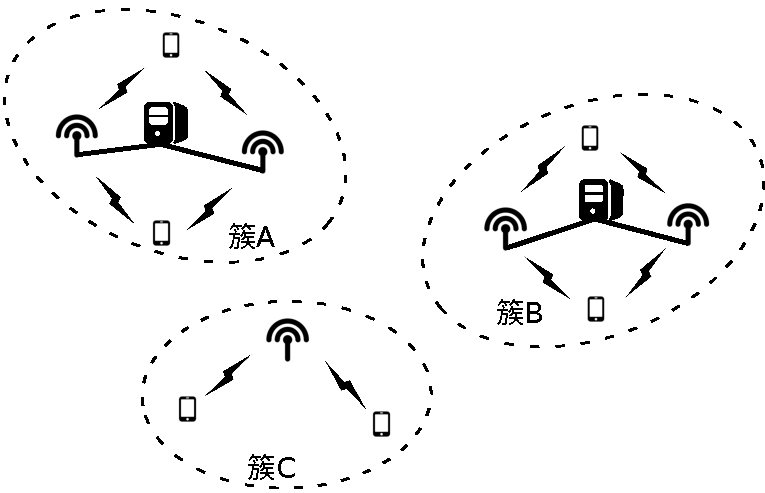
\includegraphics[width = 0.7\textwidth]{CoMP_cluster.pdf}
\caption{密集热点区域无线网络的干扰管理架构示意图}\vspace{-0.5em}
\label{CoMP_cluster}
\end{figure}
\BiSubsection{基于深度优先搜索的微基站分簇算法}{Time diversity}
根据图~\ref{e_capacity_show}~所示,相邻的基站之间如果距离过近,则由于基站之间的干扰强烈,小区中用户的遍历容量性能,
网络的覆盖率和单位面积频谱效率性能将会受到巨大的影响,除此之外,如果两个基站的距离过近,
由于微基站服务的区域用户量需求大,
容量要求高,因此两个基站之间会存在大量的边缘用户,从而极大的影响了系统的性能。

为了避免基站相聚过近而导致的基站之间的干扰强烈,边缘用户过多。
本小节提出了基于深度优先搜索的基站分簇算法。
深度优先搜索算法是计算机科学当中的基础算法,也是图论当中比较经典的算法之一。

下面介绍基于图的深度优先搜索的为基站分簇算法,为了应用按深度优先的搜索,首先需要在将网络中的基站拓扑映射成为一个图结构。
给定区域~$\mathcal{D}$~中的所有基站
~$\mathcal{S}(x,y)=\{S_1(x_1,y_1), S_2(x_2,y_2),\dots,S_i(x_i,y_i)~,\dots,S_n(x_n,y_n)\}$,
其中~$x$,$y$~分别表示基站的横,纵坐标。
对任意的~$i,j\in\{1,2,\dots,n\}$,基站~$S_i$~与基站~$S_j$~之间的距离为~$R_{ij}$,
根据微基站集合~$\mathcal{S}$~和基站之间的距离~$R_{ij}$,$i,j \in\{1,2,\dots,n\}$构造图~$\mathcal{G}$,
其中图~$\mathcal{G}$~的节点集合~$\mathcal{V}=\{v_1,v_2,\dots,v_i,\dots v_n\}$~
为微基站集合~$\mathcal{S}$~的一一映射,即对任意给定的~$i\in\{1,2,\dots,n\}$,
存在映射关系~$S_i \rightarrow v_i$。图~$\mathcal{G}$~的所有边构成的集合~$\mathcal{E}$~
根据微基站之间的距离是否小于门限~$\tau$~决定,即对任意的~$i,j\in\{1,2,\dots,n\}$,若~$R_{ij}<\tau$,
则存在边~$e_{ij}\in\mathcal{E}$,
表示图~$\mathcal{G}$~中存在边~$e_{ij}$~将节点~$v_i$~和节点~$v_j$~连接。
根据图~$\mathcal{G}$~的边集合~$\mathcal{E}$,可以构造邻接矩阵~$\mathbf{A}=\{a_{ij}\}_{n\times n}$,其中
\begin{equation}
a_{ij}=
\begin{cases}
1, & e_{ij}\in \mathcal{E}, \\
0, & e_{ij}\notin \mathcal{E}.
\end{cases}
\end{equation}

在~$\mathcal{G}$~中,定义两个节点~$v_i$~和~$v_j$~是连通的,则从定点~$i$~到定点~$j$~有路径相连。
基于深度优先搜索的基站分簇算法将所有连通的节点划归为一簇,
将图~$\mathcal{G}$~划归为由不同子图构成的不交并,
由于图上的节点和微基站之间有一一映射的关系,
属于同一个子图的节点相互连通。
可将处在同一个子图上的节点对应的基站划分成为一个簇。
即~$\mathcal{S} = \dot{\bigcup\nolimits}_{i=1}^{m}\mathcal{C}_i$,
表示将基站的集合~$S$~分成了~$m$~个子集合,每个集合里的基站构成一簇。
完整的描述如算法~\ref{algorithm_bs_dfs}~所示:


\begin{algorithm}[!htb]
\caption{ 基于深度优先搜索的基站分簇算法 }
\label{algorithm_bs_dfs}
\small
\SetKwProg{Fn}{Function}{}{end}
\KwIn{  $\tau$~;$\mathcal{S}(x,y)$}
\KwOut{ $\mathcal{K}$ }
\Begin
{
    第~1~步:初始化\\
    $\mathbf{A}=\{a_{ij}\}_{n\times n}=\{0\}_{n\times n}$~;
    $c=0$~;
    $\mathcal{K}=\varnothing$~;
    $\mathbf{v}=\{v_i\}_n=\{0\}_n$~\\

    第~2~步:构造邻接矩阵~$\mathbf{A}$:\\
    \For{~$i=1 \ to \ n$,$j=1 ~ to ~ n$~}
    {
          $a_{ij}=(\sqrt{({x_i} - {x_j})^2+(y_i-y_j)^2} < 0~)$  \\
    }
    第~3~步:构造深度优先搜索函数:\\
    \Fn{$DFS$(~$node$~$i$~, $\mathcal{C}_c$~)}
    {
      \For{~$j=1\ to\ n, j \neq i$~}
      {
        \If{~$v_j==0 \ \ and\ \ a_{ij} == 1$~}
        {
          $v_{j}=1$ \\
          $\mathcal{C}_c=\mathcal{C}_c \bigcup~ \{~S_j~\}$\\
          $\emph{DFS(~j~,~}\mathcal{C}_c ~\emph{)}$\\
        }
      }
    }
    第~4~步: 基于深度优先搜索的基站分簇\\
    \For{~$i=1 \ to \ n$~}
    {
      \If{~$v_i == 0$~}{
        $c ~+= 1$ \\
        $\mathcal{C}_c = \{~S_i~\}$\\
        $v_i = 1$\\
        $\emph{DFS(~i~,~}\mathcal{C}_c ~\emph{)}$\\
        $\mathcal{K} = \mathcal{K} \bigcup~ \{~\mathcal{C}_c~\}$\\
      }
    }
}
\end{algorithm}

算法的输入为距离门限~$\tau$和基站的坐标参数~$\mathcal{S}(x,y)$,
算法分为四个步骤执行。

其中第一步为初始化步骤,
将邻接矩阵~$\mathbf{A}$~初始化为~$\mathbf{0}_{n\times n}$,
将网络中微基站簇的个数~$c$~设置为0个,
微基站簇的集合~$\mathcal{K}$~设置为空集~$\varnothing$,
用于标识是否与微基站一一映射的节点是否访问过的向量~$\mathbf{v}$~设置为~$\mathbf{0}_{n\times 1}$,
对应位置为~0~表示未被访问,为~1~表示已经被访问。

算法的第二步为构造邻接矩阵,
对任意的基站~$S_i$~和~$S_j, ~i, ~j \in \{~1,~2,\cdots,~n~\}$,
当基站之间的距离小于门限~$\tau$,则邻接矩阵对应的位置~$a_{ij}=a_{ji}=1$,
否则邻接矩阵对应的位置~$a_{ij}=a_{ji}=0$。

算法的第三步为构造邻接矩阵的深度优先搜索的矩阵,
深度优先搜索用于将与给定的节点~$i$~的所有连通的节点全部搜索出来,构成集合~$\mathcal{C}$~。
首先将节点~$i$~对应的基站~$S_i$~放入集合~$\mathcal{C}$~中,
并将向量~$\mathbf{v}$~中的第~$i$~位~$v_i$~置~1,
接着采用递归的方法依次遍历所有除给定节点~$i$~以外的节点,
如果存在节点~$j$~与给定节点~$i$~相连通且未被遍历,
则将微基站~$S_j$~放入集合~$\mathcal{C}$~中,
并将向量~$\mathbf{v}$~中的第~$j$~位~$v_j$~置~1,
从节点~$j$~开始继续执行按深度搜索的遍历,
直到所有与给定节点~$i$~连通的节点都被找到为止。
通过深度优先搜索函数可以得到网络中的一簇基站。

算法的第四步应用第三步给出的深度优先搜索函数,从~1~到~$n$~依次开始遍历整张图,
如果节点~$i$~未被分簇,通过函数找到与节点~$i$~连通的所有节点作为一簇。
直到所有的节点均被分簇为止。


算法通过给定距离门限,将小于距离门限的所有基站连接在了一起。这些基站共同给所覆盖区域内的用户进行服务。
从而极大的降低了边缘用户的数量,增大了用户所接收到的有用功率,减小了用户接收到的干扰。

但是,由于小区中基站的部署是泊松点过程,因此,小区中的基站的分布并不均匀,
因此可能会出现某个协作集当中的基站过多,
从而可能导致多用户簇内的多用户联合传输的复杂度过高。
不仅如此,由于小区中的微基站采用了以基站为中心的分簇方式。
小区中的服务范围依然存在明显的边界,处在边界上的用户依然会可能会受到比较严重的干扰。

\BiSubsection{基于~k~-~均值的微基站分簇算法}{Time diversity}
K~-~均值算法是人工智能领域常用的一种非监督学习算法\citeup{InfoTheoryInference}。
其是一种基于迭代的统计学习方法,由~Dempster~等人总结提出,
是均方最大(~EM~)算法的一种特例\citeup{statisticslearning}。
算法的主要步骤分为两步,即分配步骤和更新步骤。
功能分别为设定权重矩阵和更新均值点集。
与机器的思考方式不同,人类可以很容易的辨识区域内的物体,并将这些物体分类。
但若要让计算机也可以对空间内的点集进行分簇,
需要采用聚类算法,将簇内基站相距距离较近,并且与簇外基站相距较远,
并且由于算法存在均值,一个簇所划归的区域近似为一个圆形。
k~-~均值算法首先随机生成~k~个点作为均值的初始点,均值点的集合用~$\mathcal{M}$~表示,
$\mathcal{M}=\{~M_1(x_1,y_1),~M_2(x_2,y_2),\dots,~M_k(x_k,y_k)~\}$。
将每个均值附近的点作为一簇,再通过簇内点集迭代出新的均值。
直到算法收敛或迭代次数耗尽为止。

在密集热点区域无线网络覆盖的区域~$\mathcal{D}$~上,
已知微基站的位置坐标集合~$\mathcal{S}(x,y) = \{S_1(x_1,y_1), S_2(x_2,y_2),\dots,S_n(x_n,y_n)\}$。
用~k~-均值算法将点集~$\mathcal{S}(x,y)$~分成~K~个簇~$\mathcal{S} = \dot{\bigcup}_{i=1}^{k} \mathcal{C}_i$。
对任意的~$i\in\{~1,~,2,\dots,~n~\}$,$j\in\{~1,~2,\dots,~k~\}$,
$d(~S_i,~M_j~)$~表示微基站~$S_i$~和均值~$M_j$~之间的距离。算法的描述如算法~\ref{kmeansalgorithm}~所示:
\begin{algorithm}[!htb]
\caption{ 基于~k~-均值聚类的基站分簇算法 }
\label{kmeansalgorithm}
\small
\SetKwProg{Fn}{Function}{}{end}
\KwIn{$k$~;$\mathcal{S}(~x,~y~)$~;$iter$}
\KwOut{$\mathcal{M}$}
\Begin
{
    第1步:初始化\\
    随机生成~k~个坐标~$\mathcal{M}=\{~M_1,~M_2,\cdots,~M_k~\}$~构成均值点集;\\
    生成权值矩阵~$\mathbf{C}=\{~0~\}_{n\times k}$~;\\
    迭代次数~$count=0$~\\

    第2步:~k~-~均值算法:\\
    \While{~$count++ < ~iter$~}
    {
      步骤~2.1:设定权重矩阵\\
      $\mathbf{C}=\{~c_{ij}~\}_{n\times k}=\{~0~\}_{n\times k}$\\
      \For{~$i=1 \ to \ n$~}
      {
        $\hat{j}=\arg\min\limits_{j} ~d(~S_i,~M_j~)$ \\
        $c_{i\hat{j}}=1$  \\
      }

      步骤~2.2~:均值点集更新:\\
      \For{~$j=1 \ to \ k$~}
      {
        $C_j = \sum_{i=1}^n c_{ij}$  \\
        $M_j(~x_j, y_j~) = \frac{\sum_{i=1}^{n} c_{ij} S_i(~x_i,~y_i~)}{C_j}$  \\
      }
    }
}
\end{algorithm}

首先输入基站分簇的簇的个数~k~,微基站的坐标~$\mathcal{S}(~x,y~)$,迭代次数~$iter$。
算法主要分为两步,第~1~步为初始化部分,随机生成~k~个点作为均值点的初值,
权重矩阵~$\mathbf{C}$~设定为全~0~矩阵,设定迭代次数~$count$~为~0。
算法的第~2~步为~k~-~均值算法的实现,是一个迭代的过程,迭代的次数为~$iter$~次。
迭代的过程分为两个子步骤,子步骤~2.1~找遍历所有的微基站,找到距离微基站最近的均值点,
将权重矩阵~$\mathbf{C}$~相应的位置置~1。
子步骤~2.2~用得到的权值矩阵~$\mathbf{W}$~
对基站的坐标~$\mathcal{S}(~x,~y~)$~进行权值更新得到新的均值集合~$\mathcal{M}$。

基于~k~-均值算法的聚类可以对基站进行分簇,与基于深度搜索算法的基站分簇不同,
基于~k~-~均值算法的基站分簇将区域内的基站均匀的分配到~k~个簇当中,
每个区域的大小也近似相同,是一种有效的基站分簇算法。
并且基于~k~-~均值的基站分簇算法可以的到网络的中心,
簇的大致位置可以通过均值的信息反映出来。

基于~k~-~均值算法的基站分簇需要预先设置好簇的个数,
为了得到最优的簇的个数,
需要进行多次试验。
不仅如此,算法需要通过迭代实现分簇,算法的复杂度较高。
由于算法并不是依据基站之间的关系进行分簇,因此也没有利用基站之间的拓扑结构这一信息。




%当用户的有用信号的信道状态信息已知的情况下,
%可以对中断概率做更准确的分析,从而得到更精确的距离门限~$\tau$。
%下面对中断概率做进一步的分析,
%根据用于服务用户的微基站~$S_0$~发射的有用信号的的发射功率~$P$,信道系数~$h$~和距最近基站的距离~$r$,有用接收功率的表示为:
%\begin{equation}
%  P_r= h r^{-\alpha} P
%\end{equation}
%因为信道状态信息已知,在不采用其他的处理手段的情况下,用户的接收功率是已知的。
%干扰基站~$S_i$~与用户之间的距离为~$R_i$,信道为瑞利分布,信道系数~$h_i$~服从单位指数分布~$h_i\sim\exp~(1)$。
%干扰基站对用户的总的干扰功率的表达式为:
%\begin{equation}
%  I_r = \sum_{S_i \in \Phi \backslash S_0} h_i R_i^{-\alpha} P
%\end{equation}



\BiSection{密集热点区域无线网络的簇内干扰消除与优化}{algorithm construction}

\BiSubsection{CRAN~架构下基于分布式预编码的簇内干扰管理}{Time diversity}
为消除密集热点区域无线网络的簇内干扰,提出基于分布式迫零预编码的干扰消除技术。
其中发射端采用~CRAN~架构,即将所有基站的基带处理单元集中在一起,构成基带处理单元池(~BBUs~),
在基站端退化为远端射频头(~RRHs~),进行模数转换与射频收发功能,并将用户的信道状态信息
传送到~BBUs,实现基于信道状态信息的迫零预编码。
簇内干扰消除的原理框图如图~\ref{precode_inner_cluster_show}~所示:
假设在一个簇内存在~$l$~个基站,在每个基站所覆盖的区域内随机选择一个用户即一个簇内
同时对~$l$~个用户进行服务。
在~BBUs~中对基带信号进行处理,待发射的信号向量为~$\mathbf{q}=\{~q_1,~q_2,\dots,~q_l~\}, ~q\in\{~\pm 1~\}$。
在基于迫零预编码的簇内干扰管理算法中,首先要给待传送的信号进行功率分配。
每个用户所分配的功率由功率分配因子~$\mathbf{p}$~决定。

\begin{figure}[htbp]
\centering
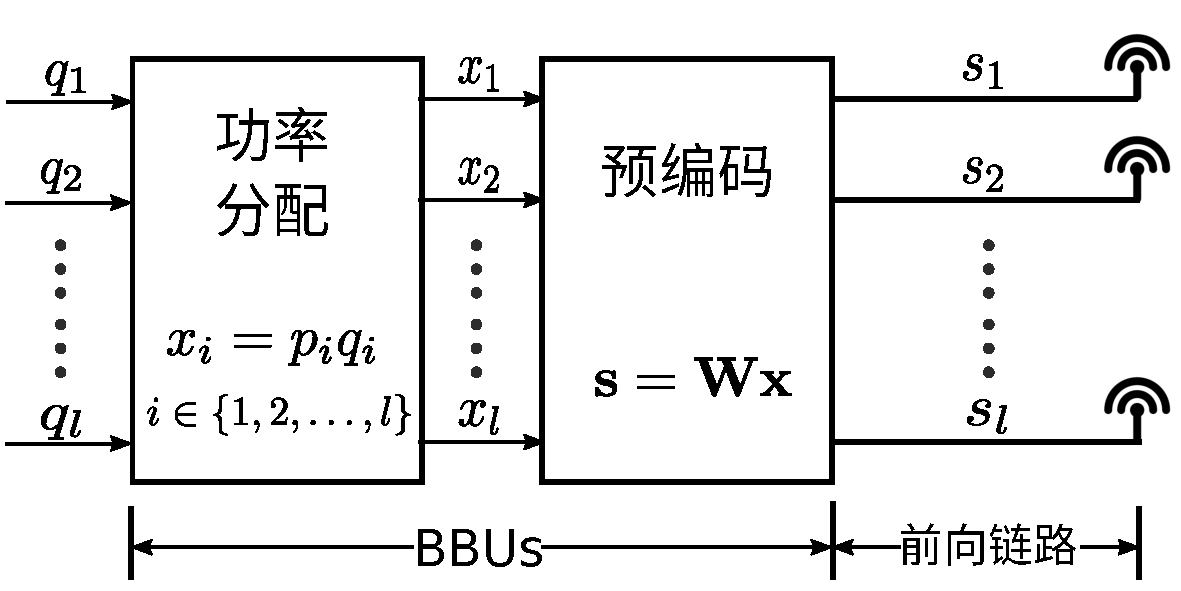
\includegraphics[width = 0.85\textwidth]{precode_inner_cluster_show.pdf}
\caption{CRAN~架构下基于分布式预编码的簇内干扰管理架构图}\vspace{-0.5em}
\label{precode_inner_cluster_show}
\end{figure}

功率分配过后的信号~$\mathbf{x}=\{~p_1q_1,~p_2q_2,~\dots,~p_nq_n~\}$。
对经过功率分配后的信号向量进行迫零预编码,得到待发送的信号~$\mathbf{s}=\mathbf{W}x$。
其中迫零预编码的预编码矩阵
~$\mathbf{W}=\mathbf{G}^{\mathrm{T}}(\mathbf{G}\mathbf{G}^{\mathrm{T}})^{-1}$。
其中~$\mathbf{G}=\{g_{ij}\}_{~l~\times~ l}=R_{ij}^{-\alpha}h_{ij}$。其中~$R_{ij}$~
为基站~$S_i$~和用户~$U_j$~之间的距离,$h_{ij}$~为瑞利信道下基站~$S_i$~和用户~$U_j$~
的信道系数。
得到了经过预编码矩阵得到的待发送信号~$\mathbf{s}=\{~s_1,~s_2,\dots,~s_l~\}$,基带信号的处理完成,
对任意的~$i\in\{~1,~2,\dots,~l~\}$,$s_i$~表示需要微基站~$S_i$~去发送的信息。
将发送信号~$\mathbf{s}$~通过前向回程链路传送给微基站~$\mathcal{S}$,
此时不同用户的信息彼此之间相互正交,因此不会受到来由于使用同时同频资源而造成的用户之间的干扰。

\BiSubsection{簇内用户的功率资源分配}{Time diversity}
根据上一小节的内容,在进行预编码之前,首先需要进行功率分配。
本小节提出等功率分配方式,分别为等功率分配和最大化基站功率使用的功率分配。
其中,等功率分配假设每个微基站的天线上所能承载的最大的功率已知,系统基于公平性的原则,
希望每个用户分配到相同的功率。
最大化功率使用的功率分配方法不需要每个用户分配到的功率均是相等的,
而是希望尽可能的使用基站的功率,从而使得所有的用户分配到的总的功率最大化。

等功率分配需要满足每个用户分配的功率是相等的。但经过预编码后信号需要满足功率约束条件。
预编码矩阵~$\mathbf{W}$~可以写成分块列向量的形式
~$\mathbf{W}=\{~\mathbf{w}_1,~\mathbf{w}_2,\dots,\mathbf{w}_l~\}$,
假设微基站所能提供的最大功率为~$P$~则功率约束条件为:
\begin{equation}\label{P_constrain}
  {s_i}^2 = (\mathbf{w}_i \mathbf{x})^2 = \sum_{j=1}^l (w_{ij} p_j q_j)^2
  = \sum_{j=1}^l (w_{ij} p_j)^2 \leq P ,~ i\in \{~1,~2, \dots, ~l~\}
\end{equation}
由于采用等功率分配,~$p_1=p_2=\cdots=p_l=p$~上式可以变形为:
\begin{equation}
  \sum_{j=1}^{l} (w_{ij}p)^2 \le P ,~ i\in \{~1,~2, \dots, ~l~\}
\end{equation}
根据功率分配约束,可以得到功率分配因子:
\begin{equation}
  p=\frac{1}{\min\{~\sum_{j=1}^{l} (w_{1j})^2,~\sum_{j=1}^{l} (w_{2j})^2,\dots,~\sum_{j=1}^{l} (w_{lj})^2~\}}
\end{equation}
由于在超密集组网场景中,网络为一个干扰受限的网络,因此对网络起主要影响的是基站之间的干扰。
而对簇内采用了迫零预编码技术,簇内用户的信息在不同的向量空间当中。
簇内的干扰完全的得到了消除,是否使得簇内和速率达到最优与否其性能的影响可以忽略不计。

\BiSection{密集热点区域无线网络优化的性能分析}{analysis}
\BiSubsection{网络分簇算法的分析}{cluster}

在第三章,我们给出了网络仿真的网络示意图~\ref{network_dis_show},
对基于深度优先搜索算法的基站分簇算法得到的分簇结果进行仿真,
仿真参数如表~\ref{dfs_show_sim_para}~所示:
\begin{table}[htbp]
\caption{基于深度优先搜索的分簇算法的仿真参数}
\label{dfs_show_sim_para}
\vspace{0.5em}\centering\wuhao
\begin{tabular}{cccc}
\toprule[1.5pt]
参量 & & & 设置 \\
\midrule[0.5pt]
基站的分布~$\Phi$~ & & & 泊松点过程 \\
泊松点过程的密度参数~$\lambda_s$~ & & & ~$0.01~\mathrm{m}^{-2}$~ \\
区域的大小  & & & ~$100\mathrm{m} \times 100 \mathrm{m}$~ \\
深度搜索的距离门限~$\tau$~ & & & ~$5\mathrm{m}$~\\
\bottomrule[1.5pt]
\end{tabular}
\end{table}

选取的区域的大小为 ~$100\mathrm{m} \times 100 \mathrm{m}$~的正方形的区域,
正方形的区域中的基站的部署为泊松点过程,密度参数为~$\lambda_s=0.01 \mathrm{m}^{-2}$,
距离门限~$\tau=5~\mathrm{m}$。
对生成的这片区域采用基于深度优先搜索的分簇算法,得到的网络示意图如图~\ref{dfs_network_show}~所示。
其中的蓝色的点表示独立的微基站,粉色的点表示使用了多用户联合传输的微基站。
如果微基站的节点之间有一条边相连,则两个基站同属于一个簇。
可以看到,当两个基站的距离~$R_{i,j} < 5$~时,基站就会被连接在一起,共同的归于一个簇。
验证了算法的正确性。
由于密集热点区域的用户具有集中性,因此当两个基站之间的距离过远时,处在边缘的用户更少。
除此之外,基站之间的距离较远,所服务的用户距离干扰基站的距离更远,有效的避免了基站相聚过近的干扰,以及处在边缘的用户的数量过多对性能的影响。

\begin{figure}[htbp]
\centering
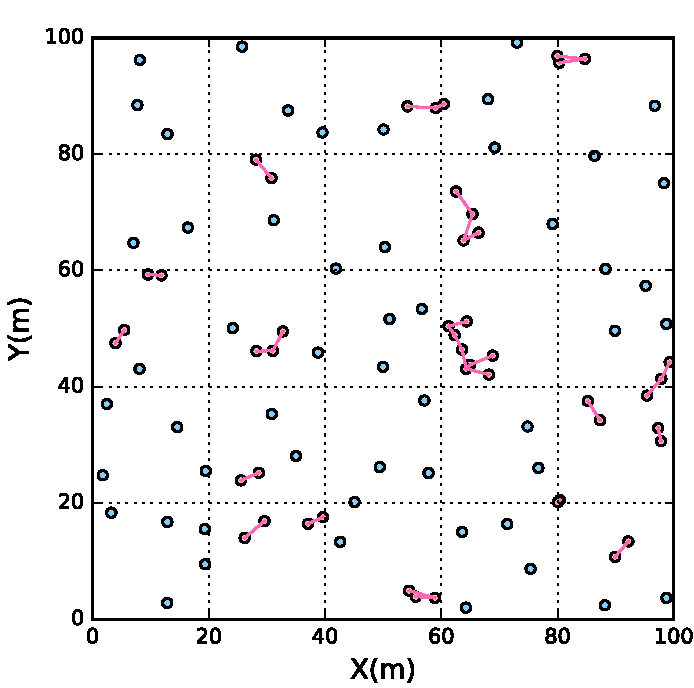
\includegraphics[width = 0.5\textwidth]{dfs_network_show.pdf}
\caption{基于深度优先搜索的分簇算法的效果图}\vspace{-0.5em}
\label{dfs_network_show}
\end{figure}

对基于~k~-~均值的基站分簇算法进行仿真
,对一片区域内的的微基站进行分簇,得到分簇结果,
仿真的参数表如表~\ref{kmeans_show_sim_para}所示:
\begin{table}[htbp]
\caption{基于~k~-~均值的分簇算法的仿真参数}
\label{kmeans_show_sim_para}
\vspace{0.5em}\centering\wuhao
\begin{tabular}{cccc}
\toprule[1.5pt]
参量 & & & 设置 \\
\midrule[0.5pt]
基站的分布~$\Phi$~ & & & 泊松点过程 \\
泊松点过程的密度参数~$\lambda_s$~ & & & ~$0.01~\mathrm{m}^{-2}$~ \\
区域的大小  & & & ~$100~\mathrm{m} \times 100~ \mathrm{m}$~ \\
簇的个数~$k$~ & & & ~$20$~\\
\bottomrule[1.5pt]
\end{tabular}
\end{table}

选取的区域的大小为~$100~\mathrm{m} \times 100~ \mathrm{m}$~的正方形区域,
正方形的区域中的基站部署为泊松点过程,密度参数~$\lambda_s=0.01~m^{-2}$,设置分簇的个数为~$20$~个。
对以泊松点过程生成的基站采用基于~k~-~均值的基站分簇算法,得到的网络示意图如图~\ref{kmeans_network_show}~所示。
可以看到整个区域被泰森多边形分割,归属于同一个泰森多边形的基站作为一簇,簇内的微基站采用多用户联合传输算法,
多边形内粉色的点表示联合起来的基站。可以看到基站均匀的被分割成了以均值为中心的区域。每个簇内大约有~5~个微基站。
\begin{figure}[htbp]
\centering
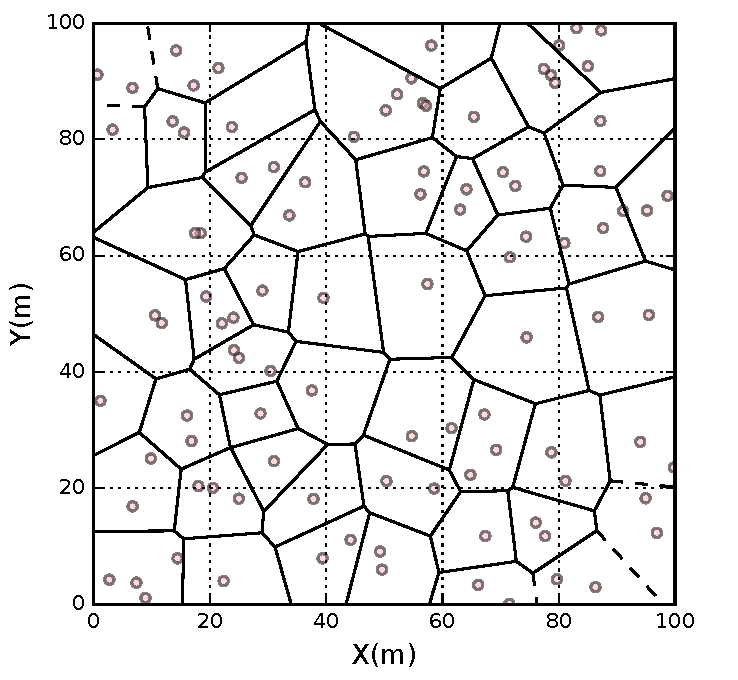
\includegraphics[width = 0.5\textwidth]{kmeans_network_show.pdf}
\caption{基于~k~-~均值的分簇算法的效果图}\vspace{-0.5em}
\label{kmeans_network_show}
\end{figure}

\BiSubsection{优化算法的性能分析}{cluster}
基于前两节的阐述和分析,这一节对密集热点区域无线网络优化后的系统性能与优化之前进行对比,
应用~Python3.5~进行仿真分析,分别仿真了基于深度优先搜索和基于~k~-~均值的基站分簇算法对基站进行分簇,
采用基于~ZFBF~的多用户联合传输干扰消除技术对网络进行优化,以覆盖率作为目标参数对系统的性能进行分析。
具体的仿真参数如表~\ref{cluster_zfbf_sim_para}~所示。
\begin{table}[htbp]
\caption{密集热点区域无线网络的性能优化的仿真参数设定}
\label{cluster_zfbf_sim_para}
\vspace{0.5em}\centering\wuhao
\begin{tabular}{cccc}
\toprule[1.5pt]
参量 & & & 设置 \\
\midrule[0.5pt]
基站的分布~$\Phi$~ & & & 泊松点过程 \\
用户的分布~$\Psi$~  & & & 混合二维高斯分布\\
用户的分散程度~$\sigma$~ & & &  ~$5\mathrm{m}$~ \\
区域~$\mathcal{D}$~的大小  & & & ~$100\mathrm{m} \times 100 \mathrm{m}$~ \\
微基站的天线数 & & & 1 \\
基站的最大发射功率~$P$~ & & & 1 \\
用户的天线数 & & & 1 \\
服务基站的选择方式 & & & 簇内多用户联合传输 \\
门限参数~$\tau$~ & & & ~$3\mathrm{m}$,~$5\mathrm{m}$,~$7\mathrm{m}$~ \\
均值个数~$k$~ & & & ~$30,~50,~70$~ \\
$\mathrm{SINR}$ & & & $-10 \sim 20$~dB \\
\bottomrule[1.5pt]
\end{tabular}
\end{table}

本章基于第~3~章提出并分析的网络模型进行优化,基站的分布为泊松点过程,用户的分布为混合二维高斯分布,
不失一般性,选取用户的分散程度~$\sigma = 5 \mathrm{m}$,
区域~$\mathcal{D}$~的大小为~$100\mathrm{m} \times 100 \mathrm{m}$,基站和用户的天线数均为~1~个,
基站的发射功率为~1,链路为下行链路,考虑的基站分簇方案分别为基于深度优先搜索和基于~k~-~均值的基站分簇策略。
簇内采用多用户联合传输,簇内随机选择用户进行服务。
对于基于深度优先搜索的微基站分簇算法,考虑门限参数为~$3\mathrm{m}$,$5\mathrm{m}$,$7\mathrm{m}$~的情况。
对于基于~k~-~均值的微基站分簇算法,考虑门限均值个数为~5,~10,~15~个的情况。

应用基于深度优先搜索的微基站分簇算法进行分簇,
采用基于~ZFBF~的簇内多用户多基站联合传输的干扰消除技术对网络的性能进行优化,
得到的性能结果仿真曲线如图~\ref{dfs_zfbf_sim_show}~所示:
\begin{figure}[htbp]
\centering
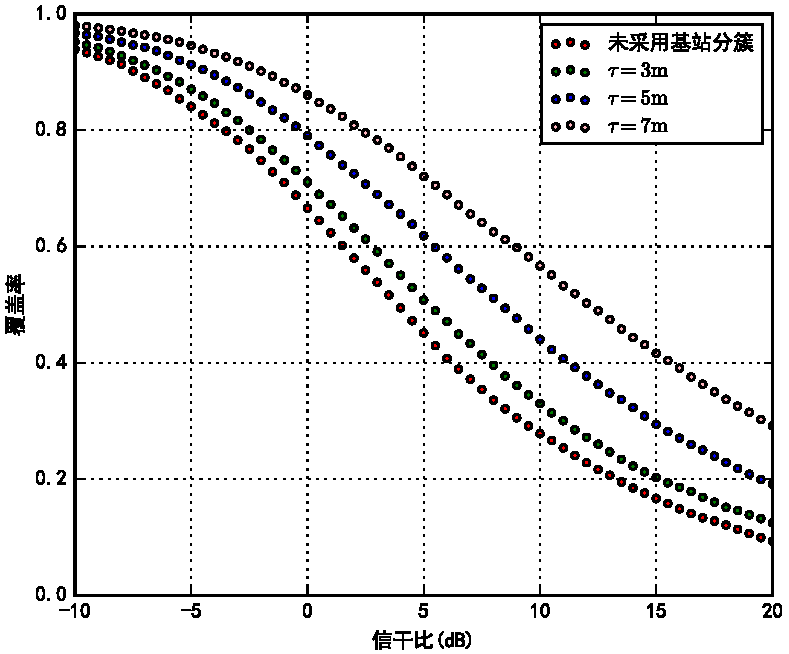
\includegraphics[width = 0.62\textwidth]{dfs_zfbf_sim_show.pdf}
\caption{基于深度优先搜索的基站分簇与多用户联合传输算法性能仿真图}\vspace{-0.5em}
\label{dfs_zfbf_sim_show}
\end{figure}
图~\ref{dfs_zfbf_sim_show}~对基于深度优先搜索的基站分簇算法的分簇策略
并基于~ZFBF~干扰消除技术进行簇内多用户联合传输这种干扰管理策略进行了仿真分析,
并与未采用基站分簇时的情况进行了比较。设定距离门限~$\tau=3\mathrm{m}$,~$5\mathrm{m}$,~$7\mathrm{m}$。

根据仿真结果可以看出,基于深度优先搜索的基站分簇算法和基于联合传输的干扰管理策略有效的提高了小区的覆盖率性能。
其中,随着距离门限~$\tau$~的提升,系统的覆盖率的性能越来越好,
但随着距离门限~$\tau$~的提升,联合的基站的个数也是逐渐提高。
系统的复杂度也逐渐提升,对~CRAN~架构的前向回程链路的容量需求也就越大。
在实际的网络中,可以根据性能和复杂度的折中合理的选择距离门限~$\tau$~这个超参数。

应用基于~k~-~均值的微基站分簇算法进行分簇,
采用基于~ZFBF~的簇内多用户多基站联合传输的干扰消除技术对网络的性能进行优化,
得到的性能结果仿真曲线如图~\ref{kmeans_zfbf_sim_show}~所示:
\begin{figure}[htbp]
\centering
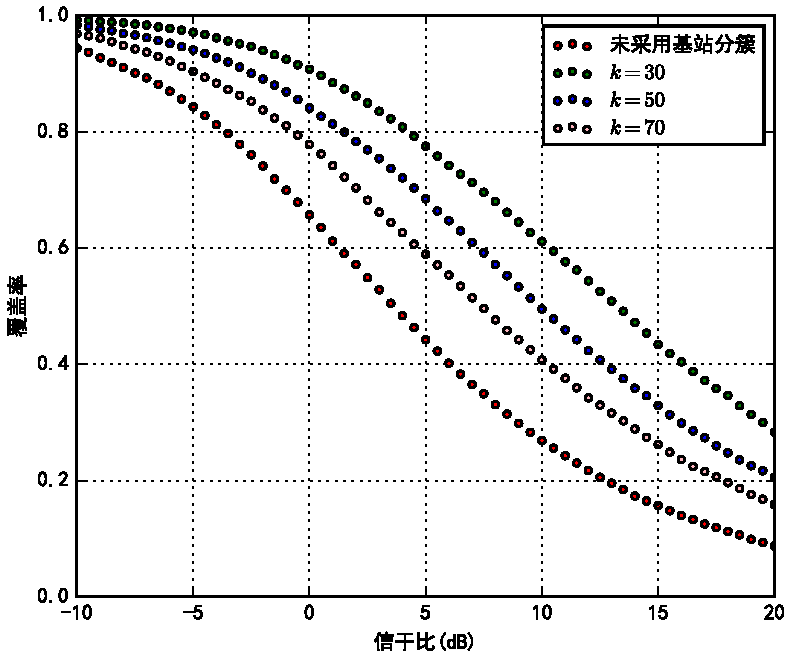
\includegraphics[width = 0.62\textwidth]{kmeans_zfbf_sim_show.pdf}
\caption{基于~k~-~均值的基站分簇与多用户联合传输算法性能仿真图}\vspace{-0.5em}
\label{kmeans_zfbf_sim_show}
\end{figure}

图~\ref{dfs_zfbf_sim_show}~对基于~k~-~均值的基站分簇算法的分簇策略
并基于~ZFBF~干扰消除技术进行簇内多用户联合传输这种干扰管理策略进行了仿真分析,
并与未采用基站分簇时的情况进行了比较,设定的均值个数分别为~$30,~50,~70$~ 个。

根据仿真结果可以看出,基于~k~-~均值的基站分簇算法进行分簇
并基于联合传输进行干扰管理有效的提高了小区的覆盖率性能。
其中,随着均值个数降低,簇的密度降低,簇内联合的基站的个数提高,系统的覆盖率的性能越来越好,
但随簇的个数降低离,联合的基站的个数也是逐渐提高,复杂度逐渐提升,系统对计算能力的需求逐渐提高,
对~CRAN~系统的前向链路的容量需求也逐渐提高。

根据第三章得到的结果,网络的单位面积谱效率是对网络的覆盖率求积分的形式,因此,网络的单位面积谱效率
和网络的中断概率是正相关的,提升了网络的覆盖率,也说明网络的单位面积谱效率也得到了提升。

\BiSubsection{不同分簇算法的优化性能对比}{cluster}

在上一小节中对比了采用相同基站分簇算法的不同的参数的性能优化效果,
本小节对比不同分簇算法下的性能优化效果。
本文采用的优化方案以基站之间相互协作,共同服务多个用户为代价,换取了区域覆盖率的提升,
因此希望尽可能少的基站数协作就能换取显著的性能提升。
图~\ref{comp_bs_number}~显示了两种分簇算法达到相同的覆盖率性能时,所需的总的基站协作的个数。
选取~0dB,3 dB,5dB~这三个典型门限指标,分析在这三个门限下的覆盖率性能,
可以看到达到相同的覆盖率性能,基于深度优先搜索的基站分簇算法所需的总共的协作基站数
小于基于~k~-~均值的基站分簇算法。
这样的结果是合理的,因为深度优先搜索把低于距离门限的所有的基站均联合在了一起,
因此有效减少了边缘用户的数目,也大大降低了微基站之间的相互干扰,但是基于~k~-~均值的微基站分簇
只是通过迭代的方法将基站均匀的分簇,
因此基于深度优先搜索的微基站分簇算法在同等的协作基站数目下性能优于基于~k~-~均值的基站分簇算法。

\begin{figure}[htbp]
\centering
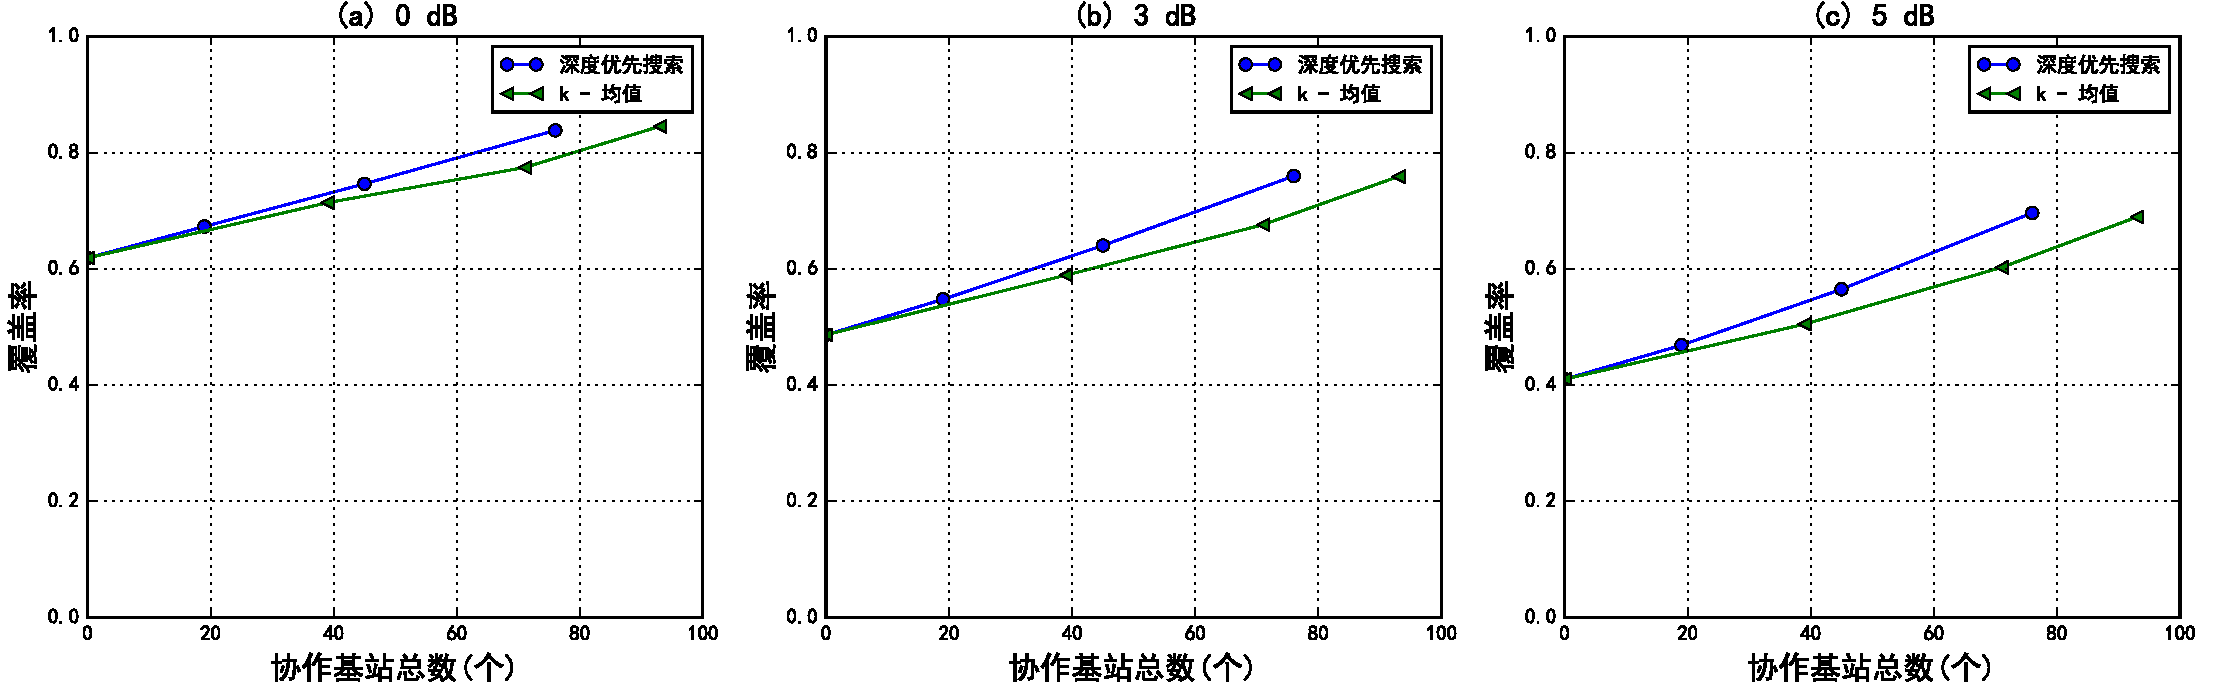
\includegraphics[width = 0.98\textwidth]{comp_bs_number.pdf}
\caption{覆盖率与总的协作基站数的关系}\vspace{-0.5em}
\label{comp_bs_number}
\end{figure}

但深度优先搜索算法是将距离低于距离门限的基站全部连接在一起,
而不规则的网络模型又是一个非均匀的网络模型,
因此会出现分簇不均匀的情况,反观~k~-~均值算法,将基站均匀的分成若干个簇,分簇更加均匀,
选取~0dB,3 dB,5dB~这三个典型门限指标,分析在这三个门限下的覆盖率性能与最多的协作基站
的个数之间的关系,得到的曲线如图~\ref{comp_max_bs_number}~所示,从图中可以看出,
随着簇内协作基站的最大值的增加,覆盖率整体呈现上升的趋势,而基于~k~-~均值的基站分簇算法相比于
基于深度优先搜索的基站分簇算法需要更少的最多基站个数达到相同的覆盖率性能。

通过本小节的分析可知,若要让基站中总的协作基站的个数更少,采用基于深度优先搜索的基站分簇算法
相比于基于~k~-~均值的基站分簇算法更好。反之,若想让网络分簇更均匀,单个簇内的基站个数更少,
则应该采用基于~k~-均值的基站分簇算法。


\begin{figure}[htbp]
\centering
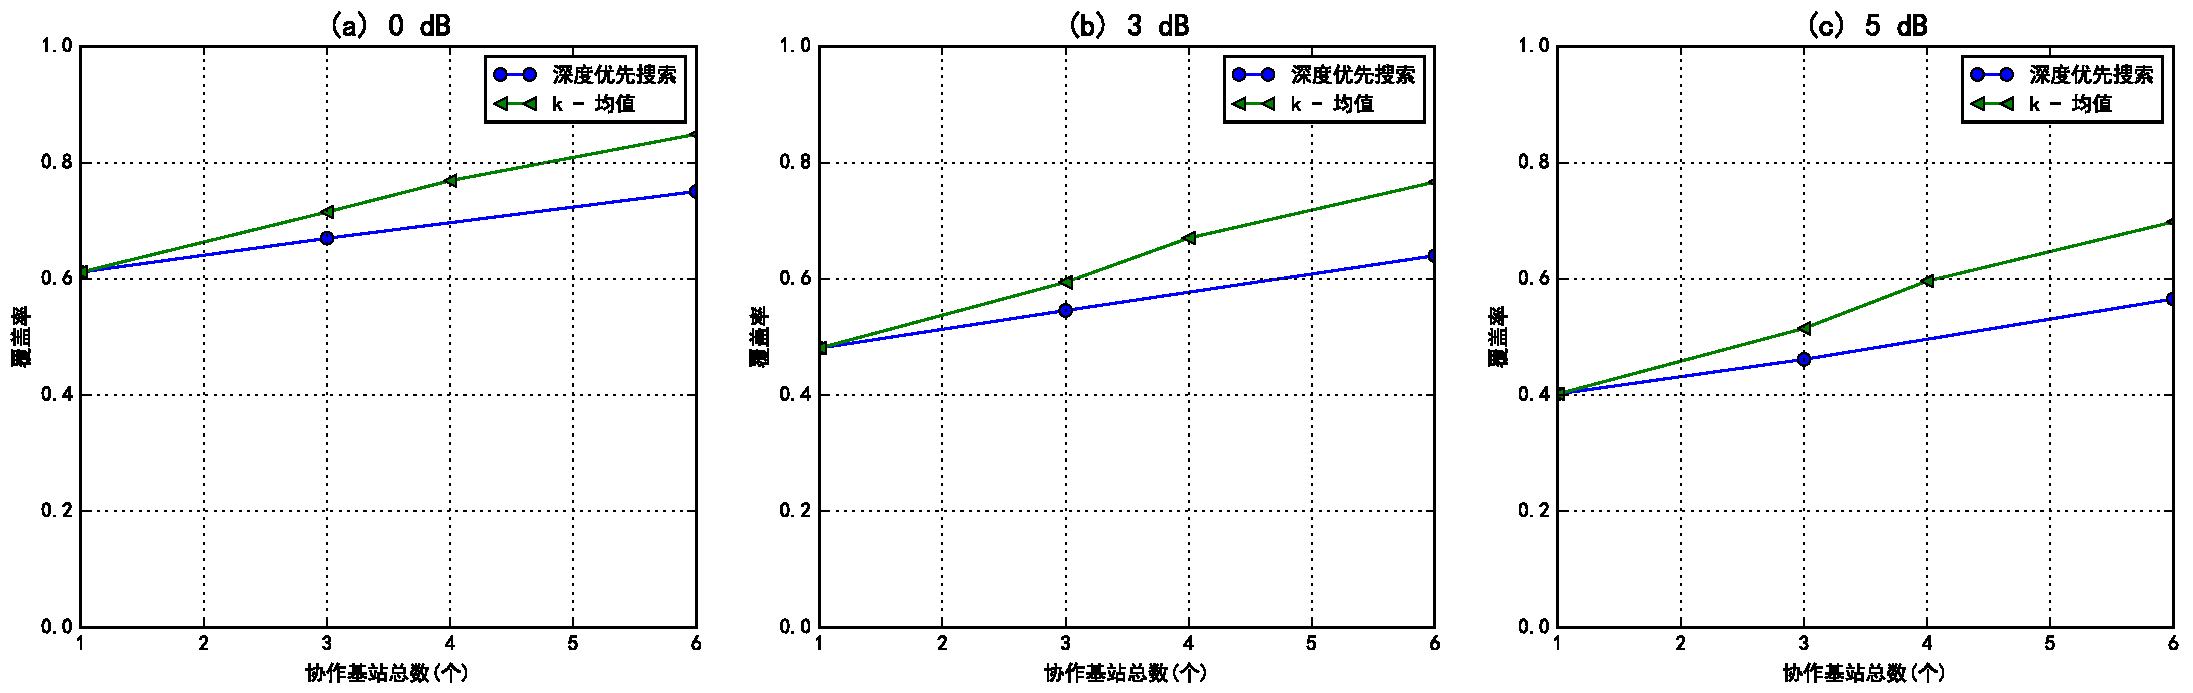
\includegraphics[width = 0.98\textwidth]{comp_max_bs_number.pdf}
\caption{覆盖率与簇内最多基站个数的关系}\vspace{-0.5em}
\label{comp_max_bs_number}
\end{figure}


\BiSection{本章小结}{Conclusion}

本章主要对密集热点区域无线网络的网络性能进行了优化,
首先,提出了两种小区内微基站的分簇算法,分别为基于深度优先搜索的微基站分簇算法,
和基于~k~-~均值的微基站分簇算法。
接着提出了多用户联合传输算法用于基站内的干扰管理,其中网络架构采用基于~CRAN~的网络架构,
簇内基站联合采用分布式~ZFBF~技术。

经过仿真实验证明,
基于首先对基站进行分簇,再对簇内进行干扰消除的干扰管理算法有效的提高了网络的覆盖率性能,
从而也说明有效的提高了网络的单位面积谱效率。

最后,对提出的两种基站分簇算法做出了比较,得到了可以出于最小协作基站数和
分簇的均匀性角度考虑,合理的选择基站分簇算法的结论。

% !Mode:: "TeX:UTF-8"

\BiAppendixChapter{结\quad 论}{Conclusions}

本文首先根据提出的密集热点区域无线网络的网络定义,
对密集热点区域无线网络进行建模,
并对该场景下的无线网络进行了性能分析,
性能指标主要为网络的遍历容量,
网络的覆盖率和网络的单位面积频谱效率。
然后根据网络的特性,提出了一种干扰管理的网络架构对网络的性能进行了优化。
网络的架构主要分为两个子部分,即首先对网络中的微基站分簇,
采用基于~ZFBF~的多用户联合传输技术实现对簇内的干扰进行消除。具体分为如下两个方面:

(1)~~根据密集热点区域无线网络的基站的拓扑结构,用户的统计特性,信道特性和网络架构对网络进行建模,
得到网络的信干噪比,遍历容量的表达式。
对密集热点区域无线网络的性能进行分析,性能的参数指标主要为网络的遍历容量,
网络的覆盖率和网络的单位面积频谱效率,得到了易于计算的网络覆盖率和网络的单位面积频谱效率的表达式,
对网络中各个位置的遍历容量,网络的覆盖率和网络的单位面积频谱效率进行了仿真和数值分析,
验证了理论分析的正确性。

(2)~~对密集热点区域无线网络进行优化,根据对密集热点区域无线网络的性能分析可知,
网络中的边缘用户受到微基站的强烈干扰,因此边缘用户的性能较差。
为了减少边缘用户,优化网络的性能,提出了网络干扰管理架构,该干扰管理架构分为两个部分,
第一个部分对基站进行分簇,提出两种微基站的分簇算法,
分别为基于深度优先搜索的微基站分簇算法和基于~k~-~均值的微基站分簇算法。
第二个部分对簇内进行干扰消除,提出采用基于~ZFBF~的簇内干扰消除算法,
该算法通过将待发送的信号在空域中对齐的方法对簇内的用户实现干扰消除。
对提出的干扰管理优化算法的性能进行仿真分析,得到的结果表明,应用了干扰管理算法的网络覆盖率性能
有明显的提升,由于单位面积频谱效率是覆盖率的积分形式,该结果也表明应用干扰管理算法对网络的性能进行优化,
也大大提升了网络的单位面积频谱效率。

本文还存在一些问题尚未解决。可以根据用户的位置和信道状态信息对簇内用户进行用户选择,进一步提升网络的性能。
可以增加网络的基站睡眠与唤醒机制,降低用户的干扰和网络的总的能耗。这些问题可以作为后续的研究方向。
   % 结论

%\BiChapter{图片的插入方法}{Methods of inserting figures}

\BiSection{单张图片的插入方法}{The method of inserting one single figure}

\BiSubsection{条标题}{The caption of subsection}

单张图片独自占一行的插入形式如图~\ref{golfer1}~所示。
\begin{figure}[htbp]
\centering
\includegraphics[width = 0.4\textwidth]{golfer}
\bicaption[golfer1]{}{打高尔夫球的人}{Fig.$\!$}{The person playing golf}\vspace{-1em}
\end{figure}

其插入图片的代码及其说明如下。
\begin{verbatim}
\begin{figure}[htbp]
\centering
\includegraphics[width=0.4\textwidth]{文件名(.eps)}
\bicaption[标签名(英文)]{}{中文标题}{Fig.$\!$}
          {English caption (首字母大写)}\vspace{-1em}
\end{figure}
\end{verbatim}
%\BiChapter{表格的绘制方法}{Methods of drawing tables}

\BiSection{普通表格的绘制方法}{Methods of drawing normal tables}


表格应具有三线表格式,因此需要调用~booktabs~宏包,其标准格式如表~\ref{table1}~所示。
\begin{table}[htbp]
\bicaption[table1]{}{符合研究生院绘图规范的表格}{Table$\!$}{Table in agreement of the standard from graduate school}
\vspace{0.5em}\centering\wuhao
\begin{tabular}{ccccc}
\toprule[1.5pt]
$D$(in) & $P_u$(lbs) & $u_u$(in) & $\beta$ & $G_f$(psi.in)\\
\midrule[1pt]
 5 & 269.8 & 0.000674 & 1.79 & 0.04089\\
10 & 421.0 & 0.001035 & 3.59 & 0.04089\\
20 & 640.2 & 0.001565 & 7.18 & 0.04089\\
\bottomrule[1.5pt]
\end{tabular}
\end{table}

其绘制表格的代码及其说明如下。
\begin{verbatim}
\begin{table}[htbp]
\bicaption[标签名]{}{中文标题}{Table$\!$}{English caption}
\vspace{0.5em}\centering\wuhao
\begin{tabular}{cc...c}
\toprule[1.5pt]
表头第1个格   & 表头第2个格   & ... & 表头第n个格  \\
\midrule[1pt]
表中数据(1,1) & 表中数据(1,2) & ... & 表中数据(1,n)\\
表中数据(2,1) & 表中数据(2,2) & ... & 表中数据(2,n)\\
...................................................\\
表中数据(m,1) & 表中数据(m,2) & ... & 表中数据(m,n)\\
\bottomrule[1.5pt]
\end{tabular}
\end{table}
\end{verbatim}
%\BiChapter{数学公式的输入方法}{Input methods of equations}

\BiSection{行内公式}{Inline mode equations}

出现在正文一行之内的公式称为行内公式,例如~$f(x)=\int_{a}^{b}\frac{\sin{x}}{x}\mathrm{d}x$。对于非矩阵和非多行形式的行内公式,一般不会使得行距发生变化。

\BiSection{行间公式}{Displaymath mode equations}

位于两行之间的公式称为行间公式,每个公式都是一个单独的段落,下边的例子是一个无编号的行间单行公式

\[
\int_a^b{f\left(x\right)\mathrm{d}x}=\lim_{\left\|\Delta{x_i}\right\|\to 0}\sum_i{f\left(\xi_i\right)\Delta{x_i}}
\]

下边的例子是一个无编号的行间多行公式(\ref{lizi})
\begin{eqnarray*}\label{lizi}
\sin 2x&=&2\sin x\cos x\\
\cos 2x&=&2\cos x^2-1=1-2\sin x^2=\cos x^2-\sin x^2
\end{eqnarray*}
%参考文献\cite{OOSTRUM01}和参考文献\citeup{wwwlixing}


%参考文献p
\defaultfont
\bibliographystyle{GBT7714-2005NLang-HIT}
\addcontentsline{toc}{chapter}{参考文献}      % 参考文献加入到中文目录
\addcontentsline{toe}{chapter}{\bfseries  References} % 参考文献加入到英文目录
\addtolength{\bibsep}{-0.8em}
%\nocite{*}  %若将此命令屏蔽掉,则未引用的文献不会出现在文后的参考文献列表中。
\bibliography{reference}
%% -*-coding: utf-8 -*-

\defaultfont
\appendix

%%%%%%%%%%%%%%%%%%%%%%%%%%%%%%%%%%%%%%%%%%%%%%%%%%%%%%%%%
\BiAppChapter{带章节的附录}{Full Appendix}%
完整的附录内容,包含章节,公式,图表等

%%%%%%%%%%%%%%%%%%%%%%%%%%%%%%%%%%%%%%%%%%%%%%%%%%%%%%%%%
\BiSection{附录节的内容}{Section in Appendix}
这是附录的节的内容

附录中图的示例:
\begin{figure}[htbp]
\centering
\includegraphics[width = 0.4\textwidth]{golfer}
\bicaption[golfer5]{}{打高尔夫球的人}{Fig.$\!$}{The person playing golf}\vspace{-1em}
\end{figure}

附录中公式的示例:
\begin{align}
a & = b \times c \\
E & = m c^2
\end{align}

%\BiAppChapter{附录二}{appendix 2}
%\BiAppChapter{附录三}{appendix 3}
    % 附录
% !Mode:: "TeX:UTF-8"

\defaultfont
\BiAppendixChapter{攻读\cxuewei 学位期间发表的论文及其他成果} {Papers
published in the period of PH.D. education}
\setlength{\parindent}{0em}

\textbf{(一)参与的科研项目及获奖情况}
\begin{publist}
\item 参与国家自然科学基金《密集组网中区域频谱效率理论上界及干扰管理算法研究》~(~项目编号:61671186~)
\end{publist}
\vfill
\hangafter=1\hangindent=2em\noindent

\setlength{\parindent}{2em}
    % 所发文章
% !Mode:: "TeX:UTF-8"

\BiAppendixChapter{哈尔滨工业大学学位论文原创性声明及使用授权说明}{Statement of copyright and Letter of authorization}
\vspace{\baselineskip}
\begin{center}\hei\xiaosan{学位论文原创性声明}\end{center}
\vspace{1em}

本人郑重声明:此处所提交的学位论文《基于~LDPC~码的~MIMO~分集系统的理论研究》,是本人在导师指导下,在哈尔滨工业大学攻读学位期间独立进行研究工作所取得的成果。据本人所知,论文中除已注明部分外不包含他人已发表或撰写过的研究成果。对本文的研究工作做出重要贡献的个人和集体,均已在文中以明确方式注明。本声明的法律结果将完全由本人承担。

\vspace{\baselineskip}
\hspace{6em}作者签名:\hfill 日期:\hspace{2.5em}年\hspace{1.5em}月\hspace{1.5em}日

\vspace{2\baselineskip}
\begin{center}\hei\xiaosan{学位论文使用授权说明}\end{center}
\vspace{1em}

学位论文是研究生在哈尔滨工业大学攻读学位期间完成的成果,知识产权归属哈尔滨工业大学。学位论文的使用权限如下:

(1)学校可以采用影印、缩印或其他复制手段保存研究生上交的学位论文, 并向国家图书馆报送学位论文;(2)学校可以将学位论文部分或全部内容编入有关数据库进行检索和提供相应阅览服务;(3)研究生毕业后发表与此学位论文研究成果相关的学术论文和其他成果时,应征得导师同意,且第一署名单位为哈尔滨工业大学。

保密论文在保密期内遵守有关保密规定, 解密后适用于此使用权限规定。

本人知悉学位论文的使用权限,并将遵守有关规定。

\vspace{1\baselineskip}
\hspace{6em}作者签名:\hfill 日期:\hspace{2.5em}年\hspace{1.5em}月\hspace{1.5em}日

\vspace{1\baselineskip}
\hspace{6em}导师签名:\hfill 日期:\hspace{2.5em}年\hspace{1.5em}月\hspace{1.5em}日
   % 承诺
% !Mode:: "TeX:UTF-8"

\BiAppendixChapter{致\quad 谢}{Acknowledgements}

感谢陈晓华教授,作为我的导师,
您不但教我们做学问,您还教诲我们做人的道理。
钦佩您不服输的精神、正派的人格、高超的学术水平和认真的态度。

感谢孟维晓教授,得益于您的帮助才让我顺利地开启了这段学术生涯。
您品格崇高、平易近人、思维敏捷、大将之风,让我非常佩服。

感谢于启月教授,遇到您是我大学以来最幸运的一件事,这或许也会一直持续下去。
我会深遵您的教诲,做一个知行合一,外圆内方的人。

感谢韩帅老师,您告诉我结果有些时候并不重要,重要的是在这个过程中积累的能力。
这在我论文撰写的后期给了我鼓舞。

感谢何晨光老师在讨论会上对我的指导。

感谢孙湘萍老师对我无微不至的照顾。

感谢陈淑怡师姐和赵天宇师姐,在小组讨论中给我提出非常宝贵的意见。

感谢孟老师大课题组中的所有人,我会继续努力,不会让大家失望。


感谢 Andrew Jeffery 先生,您的那篇惊艳的文章\citeup{ATractable} 深深地影响了我,
您文章中的公式 (2) 和 (3) 真是神来之笔。

感谢 David Mackay 先生,您的著作 \citeup{InfoTheoryInference} 是我硕士期间最喜欢的一本著作之一。
我在看书中第 22 章时想到了我毕业论文的一个重要的创新点。
除此之外,我还钦佩您知识的渊博,您的世界太丰富了,我也不应该着眼在一处,
您给了我把文章写完的勇气。得知您于 2016 年 4 月 14 日英年早逝的消息我非常悲痛,
我会努力把自己变成像您一样的学识渊博、有趣、真正爱科学的人。

如果有一个叫“憎恨”的章节与致谢相对应,我最先想到的就是 Elwyn Berlekamp 先生, 您的著作
《 Algebraic Coding Theory 》让我痴迷,书中的第 7 章我看了好几遍才粗懂其中的
奥义。真正有点看懂的那天我记忆犹新,那天我正好在当助教,老师让我看不懂就再看一遍,
那一遍我终于看懂了,就像看了一本很精彩的小说一样。然而看懂了并没有任何的用处,如果时间回到两年前,
我不想去碰那本书,毕竟世界上有意思的“小说”那么多,何必看没有什么价值的这一本。

书不成字,纸短情长。最后感谢帮助过我和默默支持我的所有人。

谨以致谢,纪念这被偷走的两年。
% 致谢

\ifxueweidoctor
% !Mode:: "TeX:UTF-8" 

\defaultfont

\BiAppendixChapter{个人简历}{Resume}

XXXX~年~XX~月~XX~日出生于~XXXX。

XXXX~年~XX~月考入~XX~大学~XX~院(系)XX~专业,XXXX~年~XX~月本科毕业并获得~XX~学学士学位。

XXXX~年~XX~月------XXXX~年~XX~月在~XX~大学~XX~院(系)XX~学科学习并获得~XX~学硕士学位。

XXXX~年~XX~月------XXXX~年~XX~月在~XX~大学~XX~院(系)XX~学科学习并获得~XX~学博士学位。

获奖情况:如获三好学生、优秀团干部、X~奖学金等(不含科研学术获奖)。

工作经历:

\vspace{3em}\noindent
\textbf{( 除全日制硕士生以外,其余学生均应增列此项。个人简历一般应包含教育经历和工作经历。)}          % 博士学位论文有个人简介
\fi

\clearpage

\end{document}
